% Options for packages loaded elsewhere
\PassOptionsToPackage{unicode}{hyperref}
\PassOptionsToPackage{hyphens}{url}
%
\documentclass[
]{book}
\usepackage{amsmath,amssymb}
\usepackage{iftex}
\ifPDFTeX
  \usepackage[T1]{fontenc}
  \usepackage[utf8]{inputenc}
  \usepackage{textcomp} % provide euro and other symbols
\else % if luatex or xetex
  \usepackage{unicode-math} % this also loads fontspec
  \defaultfontfeatures{Scale=MatchLowercase}
  \defaultfontfeatures[\rmfamily]{Ligatures=TeX,Scale=1}
\fi
\usepackage{lmodern}
\ifPDFTeX\else
  % xetex/luatex font selection
\fi
% Use upquote if available, for straight quotes in verbatim environments
\IfFileExists{upquote.sty}{\usepackage{upquote}}{}
\IfFileExists{microtype.sty}{% use microtype if available
  \usepackage[]{microtype}
  \UseMicrotypeSet[protrusion]{basicmath} % disable protrusion for tt fonts
}{}
\makeatletter
\@ifundefined{KOMAClassName}{% if non-KOMA class
  \IfFileExists{parskip.sty}{%
    \usepackage{parskip}
  }{% else
    \setlength{\parindent}{0pt}
    \setlength{\parskip}{6pt plus 2pt minus 1pt}}
}{% if KOMA class
  \KOMAoptions{parskip=half}}
\makeatother
\usepackage{xcolor}
\usepackage{color}
\usepackage{fancyvrb}
\newcommand{\VerbBar}{|}
\newcommand{\VERB}{\Verb[commandchars=\\\{\}]}
\DefineVerbatimEnvironment{Highlighting}{Verbatim}{commandchars=\\\{\}}
% Add ',fontsize=\small' for more characters per line
\usepackage{framed}
\definecolor{shadecolor}{RGB}{248,248,248}
\newenvironment{Shaded}{\begin{snugshade}}{\end{snugshade}}
\newcommand{\AlertTok}[1]{\textcolor[rgb]{0.94,0.16,0.16}{#1}}
\newcommand{\AnnotationTok}[1]{\textcolor[rgb]{0.56,0.35,0.01}{\textbf{\textit{#1}}}}
\newcommand{\AttributeTok}[1]{\textcolor[rgb]{0.13,0.29,0.53}{#1}}
\newcommand{\BaseNTok}[1]{\textcolor[rgb]{0.00,0.00,0.81}{#1}}
\newcommand{\BuiltInTok}[1]{#1}
\newcommand{\CharTok}[1]{\textcolor[rgb]{0.31,0.60,0.02}{#1}}
\newcommand{\CommentTok}[1]{\textcolor[rgb]{0.56,0.35,0.01}{\textit{#1}}}
\newcommand{\CommentVarTok}[1]{\textcolor[rgb]{0.56,0.35,0.01}{\textbf{\textit{#1}}}}
\newcommand{\ConstantTok}[1]{\textcolor[rgb]{0.56,0.35,0.01}{#1}}
\newcommand{\ControlFlowTok}[1]{\textcolor[rgb]{0.13,0.29,0.53}{\textbf{#1}}}
\newcommand{\DataTypeTok}[1]{\textcolor[rgb]{0.13,0.29,0.53}{#1}}
\newcommand{\DecValTok}[1]{\textcolor[rgb]{0.00,0.00,0.81}{#1}}
\newcommand{\DocumentationTok}[1]{\textcolor[rgb]{0.56,0.35,0.01}{\textbf{\textit{#1}}}}
\newcommand{\ErrorTok}[1]{\textcolor[rgb]{0.64,0.00,0.00}{\textbf{#1}}}
\newcommand{\ExtensionTok}[1]{#1}
\newcommand{\FloatTok}[1]{\textcolor[rgb]{0.00,0.00,0.81}{#1}}
\newcommand{\FunctionTok}[1]{\textcolor[rgb]{0.13,0.29,0.53}{\textbf{#1}}}
\newcommand{\ImportTok}[1]{#1}
\newcommand{\InformationTok}[1]{\textcolor[rgb]{0.56,0.35,0.01}{\textbf{\textit{#1}}}}
\newcommand{\KeywordTok}[1]{\textcolor[rgb]{0.13,0.29,0.53}{\textbf{#1}}}
\newcommand{\NormalTok}[1]{#1}
\newcommand{\OperatorTok}[1]{\textcolor[rgb]{0.81,0.36,0.00}{\textbf{#1}}}
\newcommand{\OtherTok}[1]{\textcolor[rgb]{0.56,0.35,0.01}{#1}}
\newcommand{\PreprocessorTok}[1]{\textcolor[rgb]{0.56,0.35,0.01}{\textit{#1}}}
\newcommand{\RegionMarkerTok}[1]{#1}
\newcommand{\SpecialCharTok}[1]{\textcolor[rgb]{0.81,0.36,0.00}{\textbf{#1}}}
\newcommand{\SpecialStringTok}[1]{\textcolor[rgb]{0.31,0.60,0.02}{#1}}
\newcommand{\StringTok}[1]{\textcolor[rgb]{0.31,0.60,0.02}{#1}}
\newcommand{\VariableTok}[1]{\textcolor[rgb]{0.00,0.00,0.00}{#1}}
\newcommand{\VerbatimStringTok}[1]{\textcolor[rgb]{0.31,0.60,0.02}{#1}}
\newcommand{\WarningTok}[1]{\textcolor[rgb]{0.56,0.35,0.01}{\textbf{\textit{#1}}}}
\usepackage{longtable,booktabs,array}
\usepackage{calc} % for calculating minipage widths
% Correct order of tables after \paragraph or \subparagraph
\usepackage{etoolbox}
\makeatletter
\patchcmd\longtable{\par}{\if@noskipsec\mbox{}\fi\par}{}{}
\makeatother
% Allow footnotes in longtable head/foot
\IfFileExists{footnotehyper.sty}{\usepackage{footnotehyper}}{\usepackage{footnote}}
\makesavenoteenv{longtable}
\usepackage{graphicx}
\makeatletter
\def\maxwidth{\ifdim\Gin@nat@width>\linewidth\linewidth\else\Gin@nat@width\fi}
\def\maxheight{\ifdim\Gin@nat@height>\textheight\textheight\else\Gin@nat@height\fi}
\makeatother
% Scale images if necessary, so that they will not overflow the page
% margins by default, and it is still possible to overwrite the defaults
% using explicit options in \includegraphics[width, height, ...]{}
\setkeys{Gin}{width=\maxwidth,height=\maxheight,keepaspectratio}
% Set default figure placement to htbp
\makeatletter
\def\fps@figure{htbp}
\makeatother
\setlength{\emergencystretch}{3em} % prevent overfull lines
\providecommand{\tightlist}{%
  \setlength{\itemsep}{0pt}\setlength{\parskip}{0pt}}
\setcounter{secnumdepth}{5}
\usepackage{booktabs}
\usepackage{amsthm}
\makeatletter
\def\thm@space@setup{%
  \thm@preskip=8pt plus 2pt minus 4pt
  \thm@postskip=\thm@preskip
}
\makeatother
\usepackage{booktabs}
\usepackage{longtable}
\usepackage{array}
\usepackage{multirow}
\usepackage{wrapfig}
\usepackage{float}
\usepackage{colortbl}
\usepackage{pdflscape}
\usepackage{tabu}
\usepackage{threeparttable}
\usepackage{threeparttablex}
\usepackage[normalem]{ulem}
\usepackage{makecell}
\usepackage{xcolor}
\ifLuaTeX
  \usepackage{selnolig}  % disable illegal ligatures
\fi
\usepackage[]{natbib}
\bibliographystyle{apalike}
\usepackage{bookmark}
\IfFileExists{xurl.sty}{\usepackage{xurl}}{} % add URL line breaks if available
\urlstyle{same}
\hypersetup{
  pdftitle={Introduction to Network Analysis in igraph},
  pdfauthor={Cynthia S. Q. Siew},
  hidelinks,
  pdfcreator={LaTeX via pandoc}}

\title{Introduction to Network Analysis in \texttt{igraph}}
\author{Cynthia S. Q. Siew}
\date{2024-10-18}

\begin{document}
\maketitle

{
\setcounter{tocdepth}{1}
\tableofcontents
}
\setcounter{section}{-1}

\chapter*{\texorpdfstring{Introduction to Network Analysis in \texttt{igraph}}{Introduction to Network Analysis in igraph}}\label{introduction-to-network-analysis-in-igraph}
\addcontentsline{toc}{chapter}{Introduction to Network Analysis in \texttt{igraph}}

\section{What is this book about?}\label{what-is-this-book-about}

Network Science is a branch of complexity science that uses methods from graph theory to study the structure and dynamics of complex systems from a wide range of topics, such as the Internet, social networks, and ecological systems. In recent years, network science approaches have achieved some level of interest from the social sciences. In my own discipline of psychology, network science has been used to study the structure of a variety of psychological networks, ranging from the human brain, cognitive and language networks, social systems, and psychometric data. The aim of this book is to introduce the basics of network analysis using the \texttt{igraph} package in R, since R is a programming language that most psychologists are already familiar with. Hence, this book is positioned more as a ``how-to'' book, and gets into the specifics of the code and programming rather than explaining how network measures can be used to explore research topics in the social sciences (for this, I strongly recommend Thomas Hills' \href{https://www.amazon.co.uk/Behavioral-Network-Science-Language-Society/dp/1108793339/}{Behavioral Network Science}).

\section{Why write this book?}\label{why-write-this-book}

Although many researchers find networks interesting and want to adopt some aspects of the network science framework into their own work, I have observed that there is a gap between that desire and the practical knowledge of how to go about doing that. In my teaching, I have also observed that students in my PL4246 Networks in Psychology course frequently struggle with the technical/programming aspects of network analysis in the R environment. As far as I can tell, there is no dedicated textbook or open workshops or freely available online resources dedicated to teaching people about how to use \texttt{igraph} for network analysis (if I am wrong, please let me know!). Personally, I have had to learn how to use \texttt{igraph} for my own research through trial and error (mostly error), and by reading the wonderful online documentation (\url{https://r.igraph.org/reference/index.html}), over a period of several years since my PhD days (and I still think that there are loads more to learn!). The \texttt{igraph} package is rich, dense, and full of useful functions and tricks, but it is difficult to learn them readily as an outsider. By writing this book, I hope that this gap can be narrowed, especially for my students and for anyone who is ``network-curious'', but struggle to have a concrete sense of what these networks look like and what useful information can be extracted from them.

\section{Acknowledgements}\label{acknowledgements}

This book is dedicated to all my PL4246 students, past and present. I have learned tremendously about the limits of my own knowledge and gaps in my teaching strategy and approach through their fierce commitment to learn about network analysis. I would like to acknowledge their contributions in shaping the structure and contents of this book.

I would also like to acknowledge the developers of \texttt{igraph} for their hard work in developing and maintaining the package over all these years.

If you have any comments about this book or spot any glaring errors (which I am sure exists in troves since this is still an evolving and growing project!), please write to me at \href{mailto:cynthia@nus.edu.sg}{\nolinkurl{cynthia@nus.edu.sg}}. Thank you :)

\section{About the author}\label{about-the-author}

Dr.~Cynthia Siew is an Assistant Professor of Psychology at the National University of Singapore. She is a psycholinguist and cognitive scientist who uses network analysis to study cognitive structures, such as the mental lexicon and semantic memory. To learn more about her research and teaching, please see \url{http://hello.csqsiew.xyz/}.

\section{Table of Contents}\label{table-of-contents}

\textbf{Section 1: Foundations for Network Analysis}

\begin{itemize}
\tightlist
\item
  Chapter 1: Installation and set up
\item
  Chapter 2: Programming and data science basics
\item
  Chapter 3: Introduction to network objects
\item
  Chapter 4: From data to networks
\item
  Chapter 5: Manipulating network objects
\end{itemize}

\textbf{Section 2: Describing the Network}

\begin{itemize}
\tightlist
\item
  Chapter 6: Macro-level network measures
\item
  Chapter 7: Micro-level network measures
\item
  Chapter 8: Meso-level network measures
\end{itemize}

\textbf{Section 3: Modeling Networks}

\begin{itemize}
\tightlist
\item
  Chapter 9: Network models (under construction)
\item
  Chapter 10: Behaviors in the network (under construction) - Tutorial 8
\end{itemize}

\textbf{Section 4: Beyond \texttt{igraph}}

\begin{itemize}
\tightlist
\item
  Chapter 11: \texttt{keyplayer} package
\item
  Chapter 12: \texttt{influenceR} package
\item
  Chapter 13: \texttt{bootnet} package
\end{itemize}

\textbf{Bonus Chapters}

\begin{itemize}
\tightlist
\item
  Chapter 14: Network visualization in \texttt{igraph}
\item
  Chapter 15: Network visualization with other packages (under construction)
\end{itemize}

\chapter{Chapter 1: Installation and set up}\label{ch1}

\section{Installing R and RStudio}\label{installing-r-and-rstudio}

Before we can get started with network analysis, we need to prepare a computing environment for doing so. We will analyze networks using the \texttt{igraph} R package, and so the very first step is to install both R and RStudio into the device that you wish to use for network analysis. It is important to note that R and RStudio are two different things that you have to install. R is the programming language itself (like Python or C++) whereas RStudio is the software application that we will use to interact with R. RStudio is known as an \emph{integrated development environment} (other examples of IDEs are Visual Studio and PyCharm).

First, install R from \url{https://www.r-project.org/}. Note that you will have to choose a CRAN mirror that you wish to download R from - which one you pick does not matter. Since I am based in Singapore I typically choose one from nearby regions (Taiwan, Korea, Japan, Indonesia, or Worldwide). Download the latest version.

Then, install RStudio from \url{https://posit.co/}. Download the correct RStudio Desktop for your computer OS. (\url{https://posit.co/download/rstudio-desktop/})

Note that both R and RStudio are free downloads. You should not need to pay for anything.

\section{RStudio Cloud}\label{rstudio-cloud}

If you do not have a computer/laptop that you are able to install programs on, you can try using \href{https://posit.cloud/}{RStudio in the cloud}. Basically, you can run RStudio on the internet without downloading anything into your computer.

The main consideration is that the free version has a cap on usage. Below is reproduced from their website (\url{https://posit.cloud/plans/free}):

\begin{quote}
``Compute hours represent how much time a project is open or running with a particular configuration, computed as (RAM + CPUs allocated) / 2 x hours. For example, working with a project for 1 hour with 1 GB of RAM and 1 CPU allocated consumes 1 project hour. The Cloud Free plan has a cap each month of 25 project hours. Once you reach the cap, you can no longer open or create projects during your current month.''
\end{quote}

\section{Installing R packages}\label{installing-r-packages}

Now that you have R and RStudio set up, let's try to install the R packages that we will use in this book. First, what is a ``R package''? Sometimes they are known as libraries, but you can think of packages/libraries as a collection of R functions that do specialized things. Because we make use of several functions from the \texttt{igraph} package to do network analysis, we need to first download \texttt{igraph}.

To download \texttt{igraph}, open RStudio and type the following into your Console (the panel with the ``\textgreater{}'' symbol - this is where you type in instructions for R to execute).

\begin{Shaded}
\begin{Highlighting}[]
\FunctionTok{install.packages}\NormalTok{(}\StringTok{"igraph"}\NormalTok{)}
\end{Highlighting}
\end{Shaded}

Be patient and wait for the package to finish downloading. After it is downloaded, we can only start using the functions in \texttt{igraph} \emph{after} we have loaded the library into our workspace. To do this, type the following into the Console:

\begin{Shaded}
\begin{Highlighting}[]
\FunctionTok{library}\NormalTok{(igraph)}
\end{Highlighting}
\end{Shaded}

If everything is working fine, you should see a plot of two connected nodes when you run the following line of code in the Console:

\begin{Shaded}
\begin{Highlighting}[]
\FunctionTok{plot}\NormalTok{(}\FunctionTok{graph\_from\_literal}\NormalTok{(A}\SpecialCharTok{{-}}\NormalTok{B))}
\end{Highlighting}
\end{Shaded}

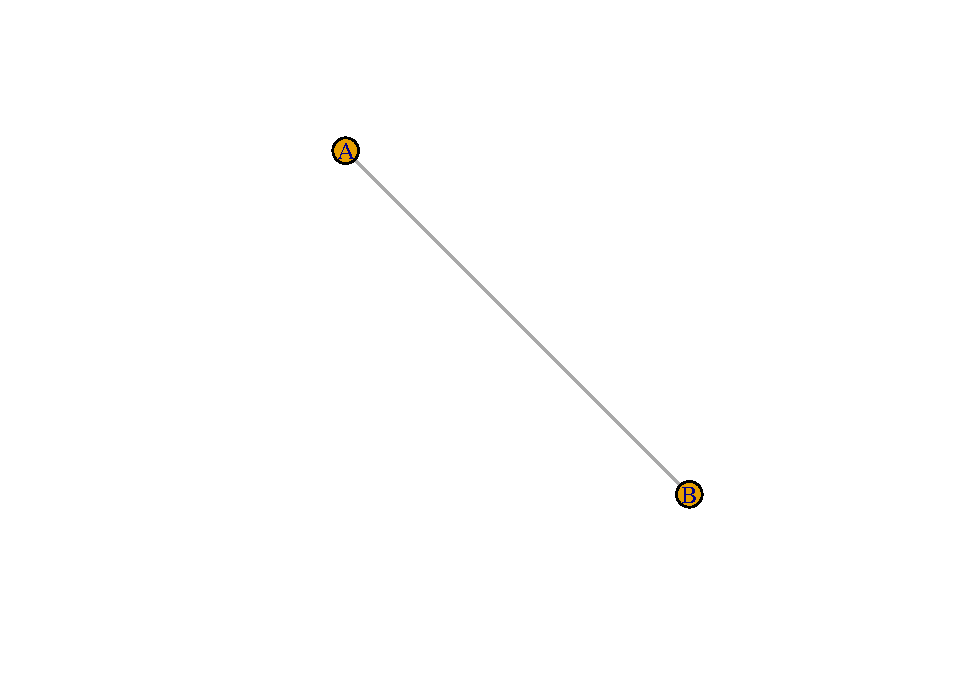
\includegraphics{bookdown-demo_files/figure-latex/unnamed-chunk-46-1.pdf}

\textbf{Important!} You only need to install a package \textbf{ONCE} (unless you wish to update it). But you will always need to load the package at the start of the R session (i.e., run \texttt{library(igraph)} in the Console whenever you open RStudio) so that you can use these special network functions.

\subsection{Exercise}\label{exercise}

\begin{enumerate}
\def\labelenumi{\arabic{enumi}.}
\item
  Try installing the package called \texttt{tidyverse}. \texttt{tidyverse} is a powerful set of packages that enable people to do cool data science things in R. It is highly recommended to learn it if you are interested in becoming a proficient user of R. See \url{https://www.tidyverse.org/} for more information.
\item
  You know if you have succeeded if you are able to load \texttt{tidyverse} into your workspace. What is the code needed to do this?
\end{enumerate}

\chapter{Chapter 2: Programming and data science basics}\label{ch2}

\section{The RStudio Environment}\label{the-rstudio-environment}

Recall from the previous chapter that R is a programming language, whereas RStudio is a program that lets you program in R in an efficient way (it is an \emph{integrated development environment}).

Once you have installed R and RStudio into your computer, you only need to open RStudio (not R) to get started.

\subsection{Setting up a Project}\label{setting-up-a-project}

A good practice before starting any kind of programming foray is to create a dedicated folder on your computer for that project, and then create a new R project that is associated with that folder. You can think of a R project as a dedicated workspace for everything that you will do in that context, which makes it easy to save your progress and return to the same state on a different day.

To create a new Project, simply go to \emph{File -\textgreater{} New Project}. Depending on whether you already have a project folder set up in your computer, you would choose either ``New Directory'' (so you create both a new folder and project file) or ``Existing Directory'' (so you navigate to the folder and create a project file for it).

You should notice in your folder a new file called \texttt{your-folder-name.Rproj}. Whenever you are done with your R session, you can choose to save all the objects in your environment (we will discuss the concepts of `objects' and `environment' in a bit) by agreeing to `Save' the prompt window. Then, when you wish to return to the project, all you have to do is to open the \texttt{your-folder-name.Rproj} and viola! All of your data objects, scripts should be right where you left it.

\begin{quote}
\emph{Try this for yourself!} Set up a new R project for a folder dedicated to this chapter and work through the contents, creating R scripts and data objects. Then, exit RStudio (remember to save the workspace image). Click on the .Rproj file to see if you are able to return to your previous workspace state.
\end{quote}

\subsection{Layout of RStudio}\label{layout-of-rstudio}

The default view of RStudio has 4 quadrants (the more useful and important tabs are mentioned below):

\begin{enumerate}
\def\labelenumi{\arabic{enumi}.}
\tightlist
\item
  Upper left: R scripts
\item
  Lower left: Console
\item
  Upper right: Environment, History
\item
  Lower right: File, Plots, Packages, Help
\end{enumerate}

Note that the positions of these quadrants may differ slightly depending on how you have set up your RStudio. You can re-size and re-organize the structure of these quadrants/panes depending on your own preferences (\emph{Tools -\textgreater{} Global Options -\textgreater{} Pane Layout}). It may also be useful for you to adjust minor things like font size and type, color themes, etc. (\emph{Tools -\textgreater{} Global Options -\textgreater{} Appearance}) to your liking, so that you feel happy and relaxed while programming.

\subsection{R scripts vs.~Console}\label{r-scripts-vs.-console}

You can enter commands (instructions to the computer) directly into the Console (where the `\textgreater{}' is) and hit Enter/Return.

Try entering the following into your Console:

\begin{Shaded}
\begin{Highlighting}[]
\DecValTok{10} \SpecialCharTok{+} \DecValTok{20}
\end{Highlighting}
\end{Shaded}

\begin{verbatim}
## [1] 30
\end{verbatim}

Notice that the answer of this math equation has been returned to you in the Console.

You can also open a blank file (\emph{File -\textgreater{} New File -\textgreater{} R Script}), write the command in it, and then execute it with \texttt{Ctrl-Enter} (Win) or \texttt{Cmd-Return} (Mac), or clicking on ``Run'' near the top right corner with the cursor on the same line. The result should also appear in the Console.

\subsection{Working with R scripts is recommended!}\label{working-with-r-scripts-is-recommended}

Where possible it is highly recommended to write your code in a R script before executing it, rather than to type it directly into the Console. This is especially true when your code becomes longer and more complex. There are also other benefits, such as:

\begin{itemize}
\tightlist
\item
  You can save your code in a .R file and re-open it in any R programming environment. This is important for reproducibility of your research.
\item
  You can leave comments in the R script to remind yourself of your work. Comments are not interpreted by R and occur after the \texttt{\#} symbol. Writing useful comments for your future self is both a skill and an art.
\item
  You can break up a complex command into multiple lines for ease of writing and editing, and then run it all by highlighting the lines and pressing Ctrl-Enter.
\end{itemize}

\begin{Shaded}
\begin{Highlighting}[]
\DecValTok{10} \SpecialCharTok{+} \DecValTok{20} \CommentTok{\# this is a comment}
\end{Highlighting}
\end{Shaded}

\begin{verbatim}
## [1] 30
\end{verbatim}

\begin{Shaded}
\begin{Highlighting}[]
\CommentTok{\# 20 * 20 (will not be run)}
\end{Highlighting}
\end{Shaded}

Advanced R users can consider using \href{https://rmarkdown.rstudio.com/articles_intro.html}{Rmarkdown} or \href{https://quarto.org/}{Quarto} for literate programming and publishing.

\section{Variables and Data Types}\label{variables-and-data-types}

\subsection{What are variables?}\label{what-are-variables}

A key aspect of programming is the ability to store information into \emph{variables}. In R sometimes these variables are also known as \emph{objects}. Try executing the following:

\begin{Shaded}
\begin{Highlighting}[]
\NormalTok{x }\OtherTok{\textless{}{-}} \DecValTok{7}
\NormalTok{my\_height }\OtherTok{\textless{}{-}} \DecValTok{163}
\end{Highlighting}
\end{Shaded}

Other than numeric data, you can also store text (character) and logical data too.

\begin{Shaded}
\begin{Highlighting}[]
\NormalTok{my\_name }\OtherTok{\textless{}{-}} \StringTok{"Cynthia"}
\NormalTok{SundayToday }\OtherTok{\textless{}{-}} \ConstantTok{FALSE}
\end{Highlighting}
\end{Shaded}

Notice the use of \texttt{\textless{}-} above: this is an \emph{assignment operator} to ``assign'' values to a name/label that you provide.

In addition, variable names should not contain any weird characters and should not begin with a number. I recommend using letters and underscores.

You should notice that while no output is printed to the console, there are new lines in the Environment tab of RStudio. Have a look and see if the items make sense to you. Basically, by running the above code, the value of \texttt{x} and \texttt{my\_height} (as well as \texttt{my\_name} and \texttt{SundayToday}) has been stored in the ``memory'' of RStudio.

Then you can begin to do interesting things with the variables:

\begin{Shaded}
\begin{Highlighting}[]
\CommentTok{\# what is Cynthia\textquotesingle{}s height in metres?}
\NormalTok{my\_height}\SpecialCharTok{/}\DecValTok{100}
\end{Highlighting}
\end{Shaded}

\begin{verbatim}
## [1] 1.63
\end{verbatim}

\begin{Shaded}
\begin{Highlighting}[]
\NormalTok{my\_height }\SpecialCharTok{*}\NormalTok{ x }\CommentTok{\# a random math equation }
\end{Highlighting}
\end{Shaded}

\begin{verbatim}
## [1] 1141
\end{verbatim}

\begin{Shaded}
\begin{Highlighting}[]
\NormalTok{SundayToday }\CommentTok{\# this just prints the value of the variable }
\end{Highlighting}
\end{Shaded}

\begin{verbatim}
## [1] FALSE
\end{verbatim}

\subsection{Removing objects}\label{removing-objects}

If your workspace/environment gets too messy, you can remove variables by using the \texttt{rm()} function:

\begin{Shaded}
\begin{Highlighting}[]
\FunctionTok{rm}\NormalTok{(x)}
\end{Highlighting}
\end{Shaded}

Notice that \texttt{x} is missing from the Environment tab.

To remove everything in the Environment, click on the Broom icon in the Environment tab or use the following command \texttt{rm(list=ls())}.

\subsection{Saving objects}\label{saving-objects}

Although it doesn't make sense to save variables that contain only one value, it is useful to save variables that are more complex (e.g., data frames or network objects), and to save the entire workspace so that you can come back to your project later.

Here is how you do it:

\begin{Shaded}
\begin{Highlighting}[]
\CommentTok{\# single objects }
\FunctionTok{save}\NormalTok{(my\_height, }\AttributeTok{file =} \StringTok{\textquotesingle{}CS\_height.RData\textquotesingle{}}\NormalTok{)}

\CommentTok{\# entire workspace}
\FunctionTok{save.image}\NormalTok{(}\AttributeTok{file =} \StringTok{\textquotesingle{}everything.RData\textquotesingle{}}\NormalTok{)}
\end{Highlighting}
\end{Shaded}

Notice that you need to specify a \texttt{file} argument which is the name of the file that you want to save the information to, and that the file extension is \texttt{.RData}.

You can also save all of the objects in the workspace by clicking on the Floppy Disk icon in the Environment tab (NOT the Scripts tab).

Recall from `Setting up a Project' that you are automatically prompted to save all of the objects in the workspace before exiting the R session - this creates a hidden file called \texttt{.RData} where the information is saved to and is automatically loaded when you start a new session for the same project.

\subsection{Loading objects}\label{loading-objects}

First, wipe the Environment with the Broom icon. The Environment should be empty. Then run the following:

\begin{Shaded}
\begin{Highlighting}[]
\FunctionTok{load}\NormalTok{(}\StringTok{\textquotesingle{}everything.RData\textquotesingle{}}\NormalTok{)}
\end{Highlighting}
\end{Shaded}

All your variables have magically returned!

\subsection{What are vectors?}\label{what-are-vectors}

Vectors are a kind of a special variable that can store multiple values or data points, instead of just one.

\begin{Shaded}
\begin{Highlighting}[]
\NormalTok{a\_vector }\OtherTok{\textless{}{-}} \FunctionTok{c}\NormalTok{(}\DecValTok{1}\NormalTok{,}\DecValTok{9}\NormalTok{,}\DecValTok{6}\NormalTok{,}\DecValTok{8}\NormalTok{)}

\NormalTok{a\_vector}
\end{Highlighting}
\end{Shaded}

\begin{verbatim}
## [1] 1 9 6 8
\end{verbatim}

Notice the use of a special function \texttt{c()} to combine single values into the vector.

\subsection{Cool things you can do with vectors}\label{cool-things-you-can-do-with-vectors}

Here are some interesting things you can do with vectors - try running each command and see if you can figure out what it does by examining the output. The comments below give you several hints!

\begin{Shaded}
\begin{Highlighting}[]
\CommentTok{\# extraction}
\NormalTok{a\_vector[}\DecValTok{3}\NormalTok{]}
\end{Highlighting}
\end{Shaded}

\begin{verbatim}
## [1] 6
\end{verbatim}

\begin{Shaded}
\begin{Highlighting}[]
\CommentTok{\# removal }
\NormalTok{a\_vector[}\SpecialCharTok{{-}}\DecValTok{2}\NormalTok{]}
\end{Highlighting}
\end{Shaded}

\begin{verbatim}
## [1] 1 6 8
\end{verbatim}

\begin{Shaded}
\begin{Highlighting}[]
\NormalTok{a\_vector[}\SpecialCharTok{{-}}\NormalTok{(}\DecValTok{1}\SpecialCharTok{:}\DecValTok{3}\NormalTok{)] }\CommentTok{\# this removes the first 3 elements}
\end{Highlighting}
\end{Shaded}

\begin{verbatim}
## [1] 8
\end{verbatim}

\begin{Shaded}
\begin{Highlighting}[]
\CommentTok{\# editing}
\NormalTok{a\_vector[}\DecValTok{1}\NormalTok{] }\OtherTok{\textless{}{-}} \DecValTok{0}

\NormalTok{a\_vector}
\end{Highlighting}
\end{Shaded}

\begin{verbatim}
## [1] 0 9 6 8
\end{verbatim}

\begin{Shaded}
\begin{Highlighting}[]
\CommentTok{\# naming}
\FunctionTok{names}\NormalTok{(a\_vector) }\OtherTok{\textless{}{-}} \FunctionTok{c}\NormalTok{(}\StringTok{\textquotesingle{}a\textquotesingle{}}\NormalTok{, }\StringTok{\textquotesingle{}b\textquotesingle{}}\NormalTok{, }\StringTok{\textquotesingle{}c\textquotesingle{}}\NormalTok{, }\StringTok{\textquotesingle{}d\textquotesingle{}}\NormalTok{)}

\NormalTok{a\_vector}
\end{Highlighting}
\end{Shaded}

\begin{verbatim}
## a b c d 
## 0 9 6 8
\end{verbatim}

A key concept is the use of {[}square brackets{]} to subset the vector based on the order of the elements in the vector (numbered from left to right starting with 1).

\section{Functions and Arguments}\label{functions-and-arguments}

\subsection{What are functions?}\label{what-are-functions}

You can think of functions as special instructions that R knows of that you can use as shortcuts to do something. In fact, you have already been using a number of functions: \texttt{load(...)}, \texttt{rm(...)}, \texttt{save(...)}. The clue is that functions have a name that is typed out and has brackets following it.

\subsection{What are arguments?}\label{what-are-arguments}

Again, you already have been using arguments in functions. For instance, \texttt{load(\textquotesingle{}everything.RData\textquotesingle{})} has the argument inside the brackets which is the name of the file that you wish to load into your workspace.

The clue is that arguments are found inside the brackets of functions. You can think of arguments as additional instructions or parameters that will inform the function what it should do in specific ways.

\subsection{Multiple arguments}\label{multiple-arguments}

Some functions can take on several arguments. When this is the case, it is good practice to explicitly name the argument.

Consider the following:

\begin{Shaded}
\begin{Highlighting}[]
\FunctionTok{round}\NormalTok{(}\AttributeTok{x =} \FloatTok{131.485783}\NormalTok{, }\AttributeTok{digits =} \DecValTok{1}\NormalTok{)}
\end{Highlighting}
\end{Shaded}

\begin{verbatim}
## [1] 131.5
\end{verbatim}

\texttt{round()} is a function that takes two arguments, the first argument (\emph{x}) is the number that is being rounded, and the second argument (\emph{digits}) indicating the number of decimal places.

If you don't specify the argument names, then R assumes that they follow the internal expected order:

\begin{Shaded}
\begin{Highlighting}[]
\FunctionTok{round}\NormalTok{(}\FloatTok{131.485783}\NormalTok{, }\DecValTok{1}\NormalTok{)}
\end{Highlighting}
\end{Shaded}

\begin{verbatim}
## [1] 131.5
\end{verbatim}

\begin{Shaded}
\begin{Highlighting}[]
\CommentTok{\# try the following and think about the output}
\FunctionTok{round}\NormalTok{(}\FloatTok{131.485783}\NormalTok{, }\DecValTok{2}\NormalTok{)}
\end{Highlighting}
\end{Shaded}

\begin{verbatim}
## [1] 131.49
\end{verbatim}

\begin{Shaded}
\begin{Highlighting}[]
\FunctionTok{round}\NormalTok{(}\DecValTok{1}\NormalTok{, }\FloatTok{131.485783}\NormalTok{)}
\end{Highlighting}
\end{Shaded}

\begin{verbatim}
## [1] 1
\end{verbatim}

\begin{Shaded}
\begin{Highlighting}[]
\FunctionTok{round}\NormalTok{(}\FloatTok{131.485783}\NormalTok{)}
\end{Highlighting}
\end{Shaded}

\begin{verbatim}
## [1] 131
\end{verbatim}

For the final command, if no argument is specified (in the second location) and there is a default value (here it is 0), then R will use the default. To find out about the internal ordering of arguments and default values for any function, you can search for the function name in the Help tab, or type \texttt{?function\_name} into the Console. This gives you handy documentation about a specific function that you can quickly review.

\section{File Paths and Working Directory}\label{file-paths-and-working-directory}

\subsection{Navigation in computers}\label{navigation-in-computers}

All of your digital data in computers are stored in folders and sub-folders. When you want open a file in a program, you need to navigate to the location where that specific file is stored.

Similarly, when programming in R, if you want to load datasets and/or previously saved workspaces into your workspace you need to first ``point'' RStudio to the correct location where these files are stored.

\subsection{Helping RStudio find your stuff}\label{helping-rstudio-find-your-stuff}

First you need to know where it is currently looking at (i.e., your current \emph{working directory}):

\begin{Shaded}
\begin{Highlighting}[]
\FunctionTok{getwd}\NormalTok{()}
\end{Highlighting}
\end{Shaded}

\begin{verbatim}
## [1] "/home/cynthia/Documents/Research-Workspace/intro-to-igraph"
\end{verbatim}

Make a new folder called ``test\_folder'' in that location (using Finder or Files in your computer system). For learning purposes you can also move the \texttt{everything.RData} file there. Then try out the following:

\begin{Shaded}
\begin{Highlighting}[]
\FunctionTok{load}\NormalTok{(}\StringTok{\textquotesingle{}everything.RData\textquotesingle{}}\NormalTok{) }\CommentTok{\# notice that this does not work }

\CommentTok{\# let\textquotesingle{}s have RStudio look in the correct folder }
\FunctionTok{setwd}\NormalTok{(}\StringTok{\textquotesingle{}./test\_folder\textquotesingle{}}\NormalTok{) }\CommentTok{\# note that in Windows you will need backslashes instead}
\CommentTok{\# the period means "from the current location"}

\FunctionTok{getwd}\NormalTok{() }\CommentTok{\# this should be updated }

\FunctionTok{load}\NormalTok{(}\StringTok{\textquotesingle{}everything.RData\textquotesingle{}}\NormalTok{) }\CommentTok{\# does it work now? }
\end{Highlighting}
\end{Shaded}

Now when you place a \texttt{.RData} file in \texttt{test\_folder} you should be able to load it into your workspace.

An alternate (and possibly more intuitive) solution via the GUI is to do the either of the following: (1) \emph{Session -\textgreater{} Set Working Directory -\textgreater{} Choose Working Directory} or (2) Files tab: navigate to desired location and click on the Gear icon. Then choose ``Set Working Directory''.

Note that when you are working in a dedicated R project workspace, the default working directory is basically the project folder where the .Rproj file lives in. If you have set up the workspace as recommended in ``Setting up a Project'', then the easier approach is to simply move any data files that you need for your project into that folder, rather than to keep changing the working directory to ``find'' your files. This is good practice in any case; better to consolidate all the files associated with a given project rather than have them scattered across multiple folders.

\section{Packages}\label{packages}

\subsection{What are packages/libraries?}\label{what-are-packageslibraries}

Packages contain a set of dedicated functions, sometimes they are often called ``libraries''. While many packages come pre-installed with R, many other packages (especially the ones we need for this class) need to be installed from CRAN before we can start to use them.

\subsection{Installation vs.~Loading}\label{installation-vs.-loading}

Remember that you only need to install a package once, but you need to load them each time you begin a new RStudio session so that you can use the special functions of that package.

\begin{Shaded}
\begin{Highlighting}[]
\CommentTok{\# install ONCE}
\FunctionTok{install.packages}\NormalTok{(}\StringTok{\textquotesingle{}igraph\textquotesingle{}}\NormalTok{)}

\CommentTok{\# load EACH TIME}
\FunctionTok{library}\NormalTok{(igraph)}
\end{Highlighting}
\end{Shaded}

You can also install and load packages via the Packages tab in RStudio. Click on ``Install'' and search for the package you need. Then you can search for the packages installed on your system and load the ones you want with the check box. It is also convenient to Update packages here.

\subsection{Detaching packages}\label{detaching-packages}

If you need to remove an already loaded package in your workspace, you can uncheck the package name in Packages tab.

Or you can run the following in your console:

\begin{Shaded}
\begin{Highlighting}[]
\FunctionTok{detach}\NormalTok{(}\StringTok{"package:igraph"}\NormalTok{, }\AttributeTok{unload=}\ConstantTok{TRUE}\NormalTok{)}
\end{Highlighting}
\end{Shaded}

\section{Special Datatypes}\label{special-datatypes}

So far we know that we can store single values as objects or variables in RStudio, as well as a group of values in a vector. In this module you are also going to run into two special variable types: \emph{dataframes} and \emph{igraph network objects}. We will discuss network objects in the next chapter.

\subsection{Dataframes}\label{dataframes}

A data frame is a rectangular, 2-dimensional variable with multiple rows and columns. You should be familiar with this type of data from introductory statistics where you would load such data from Excel (or some other spreadsheet program) into SPSS or JASP for analysis.

\subsection{Loading data into RStudio}\label{loading-data-into-rstudio}

First, the data should be saved as a \texttt{.csv} file. This is basically a ``text'' version of the Excel format (look at Save As\ldots{} in your Excel program). I recommend this because special packages and functions are needed to load data from proprietary file formats. The csv format is much more flexible (it would also work with SPSS/JASP).

To see this in action, first create a .csv file called \texttt{numbers.csv} using your preferred spreadsheet program. Make two columns of random numbers and provide column headers. An example is shown below:

\begin{longtable}[]{@{}ll@{}}
\toprule\noalign{}
Column A & Column B \\
\midrule\noalign{}
\endhead
\bottomrule\noalign{}
\endlastfoot
1 & 4 \\
2 & 5 \\
3 & 6 \\
\end{longtable}

Save this file into your current working directory.

To load the file via the Console:

\begin{Shaded}
\begin{Highlighting}[]
\NormalTok{my\_data }\OtherTok{\textless{}{-}} \FunctionTok{read.csv}\NormalTok{(}\StringTok{\textquotesingle{}numbers.csv\textquotesingle{}}\NormalTok{, }\AttributeTok{header =} \ConstantTok{TRUE}\NormalTok{)}
\end{Highlighting}
\end{Shaded}

Notice that we are using a function called \texttt{read.csv} to read in .csv files (there are other functions for other kinds of files but we will mostly work with .csv files in this book). This function contains two arguments: the name of the file in the first position, and a second argument which states that there are column headers in the file. If there are no column headers, then switch this to \texttt{FALSE} and R will automatically provide labels. Finally, we assign the contents of the .csv file to a data frame object called \texttt{my\_data}, which now shows up in the Environment tab. You are of course free to change this to a different label that describes your data better.

There is an alternative approach using the RStudio GUI. To load the file via the GUI: Navigate to the file on Files tab, click on file and select ``Import Dataset''. A helpful window opens to preview how the data will look like, and gives you options to change the name of the data object, specify if there are column names/headers, etc.

\begin{quote}
Common mistake: Selecting ``View File'' opens the data as a window in RStudio, but does NOT actually load the information into the workspace, which means that you are unable to manipulate the data in any way.
\end{quote}

\chapter{Chapter 3: Introduction to network objects}\label{ch3}

\section{What is a network?}\label{what-is-a-network}

A network consists of two sets of entities: A list of \emph{nodes} and a list of \emph{edges}. Nodes correspond to the individual elements whose pairwise relational structure is specified by edges or links. So, if node A and node B are related to each other based on some criteria set by the modeler (you!) then you would specify an edge between nodes A and B.

When networks are small (on the order of a handful of nodes), it would not too be difficult to manually specify the list of nodes and their connections. However, this quickly gets too onerous once the number of nodes increases because the number of possible edges increases exponentially. For instance, a network of 5 nodes could have a maximum of 10 edges, whereas a network of 50 nodes could have a maximum of 1,225 edges.

In practice, the networks that a social scientist are likely to be working with are going to be quite large, and the networks are derived from large datasets that are external to the R programming environment. In the next chapter we will explore how to get these datasets into RStudio and how to convert them into network. In this chapter, we focus on understanding the structure of the network object, a special datatype that \texttt{igraph} uses for network analysis.

\section{Your first network}\label{your-first-network}

Network objects are a special variable that can only be analyzed with functions from the \texttt{igraph} library (that you previously installed).
Let's check out a simple example.

\begin{Shaded}
\begin{Highlighting}[]
\FunctionTok{library}\NormalTok{(igraph) }\CommentTok{\# remember that we need to load this}

\CommentTok{\# create a network of 2 nodes that are connected}
\NormalTok{g }\OtherTok{\textless{}{-}} \FunctionTok{graph\_from\_literal}\NormalTok{(}\StringTok{\textquotesingle{}cat\textquotesingle{}}\SpecialCharTok{{-}}\StringTok{\textquotesingle{}bat\textquotesingle{}}\NormalTok{)}
\end{Highlighting}
\end{Shaded}

\texttt{graph\_from\_literal} is a special function that allows the user to quickly build small networks by explicitly stating the nodes and edges of the network. Here we are creating a network of 2 nodes, labeled `cat' and `bat', and these 2 nodes are connected to each other.

You should find a new object \texttt{g} in Environment. But the description of the object does not seem like a network. That is OK! R knows what it is.

When we print \texttt{g} in the Console, we find that it has a number of special properties. If you don't want to see all the edges being printed, you can type \texttt{summary(g)} instead.

\begin{Shaded}
\begin{Highlighting}[]
\NormalTok{g}
\end{Highlighting}
\end{Shaded}

\begin{verbatim}
## IGRAPH 908e438 UN-- 2 1 -- 
## + attr: name (v/c)
## + edge from 908e438 (vertex names):
## [1] cat--bat
\end{verbatim}

\begin{Shaded}
\begin{Highlighting}[]
\FunctionTok{summary}\NormalTok{(g)}
\end{Highlighting}
\end{Shaded}

\begin{verbatim}
## IGRAPH 908e438 UN-- 2 1 -- 
## + attr: name (v/c)
\end{verbatim}

Let's try to make sense of the output in Console when we ``print'' the network object \texttt{g}.

This first line already packs a ton of information:

\texttt{IGRAPH\ f977daf\ UN-\/-\ 2\ 1\ -\/-}

\begin{enumerate}
\def\labelenumi{\arabic{enumi}.}
\tightlist
\item
  The IGRAPH label is a good sign, it means that this object is need a network object that \texttt{igraph} understands. This is followed by a UUID generated to uniquely identify the graph.
\item
  The first letter in caps can either be \textbf{D} or \textbf{U}, which corresponds to \emph{Directed} or \emph{Undirected} edges, respectively. In this example we have a \textbf{U}, which means that the edges in this network are undirected.
\item
  The second letter in caps can either be \textbf{N} or \textbf{-}, which corresponds to nodes either having \emph{Names} or are left unlabeled, respectively. In this example we have a \textbf{N}, which means that the nodes are labeled.
\item
  The third letter in caps: \textbf{W} or \textbf{-}, which corresponds to edges either having \emph{Weights} or are unweighted, respectively. In this example we have a \textbf{-}, which means that the nodes are unweighted.
\item
  It is worth noting that it is possible to have a fourth letter, \textbf{B} or \textbf{-}, which corresponds to the network being a \emph{Bipartite} graph or not, respectively. We do not cover bipartite networks in this book (for now), and so we should expect to see a \textbf{-}, as we do in this example.
\item
  The first number refers to the number of nodes.
\item
  The second number refers to the number of edges.
\end{enumerate}

\begin{quote}
A good tip for network analysis is to always check the summary of the network object to make sure that the network that you are analyzing is indeed what you think it is. For instance, if you wanted to analyze a network with weighted edges, but do not see the \textbf{W} in your network summary, this indicates that \texttt{igraph} is not interpreting the network as a weighted graph and suggests that something went wrong during the network construction/specification phase.
\end{quote}

The second line reads:

\texttt{+\ attr:\ name\ (v/c)}

This prints a list of the various node, edge, or network-level attributes associated with the network. You can think of ``attributes'' like ``properties'' of the nodes and edges. Here we have a single attribute, labeled `name', and it is a node (\textbf{v}ertex) attribute of \textbf{c}haracter class. This can be inferred from `(v/c)' following `name'.

It is possible for edges to have attributes, and for the network itself to have attributes. These will be labeled with \emph{e} and \emph{g} respectively in the character \emph{before} the forward slash.

It is possible for the attribute to take on various data classes, such as numeric, character, logical. These will be labeld with \emph{n}, \emph{c}, and \emph{l} respectively in the character \emph{after} the forward slash.

The final lines read:

\begin{verbatim}
+ edge from f977daf (vertex names):
[1] cat--bat
\end{verbatim}

This simply prints out all of the edges in the network, and this output will be truncated for very large network.

\section{Your second network}\label{your-second-network}

To broaden our understanding, let's create a slightly different network and explore its properties.

\begin{Shaded}
\begin{Highlighting}[]
\CommentTok{\# let\textquotesingle{}s create a slightly different network}
\NormalTok{g\_directed }\OtherTok{\textless{}{-}} \FunctionTok{graph\_from\_literal}\NormalTok{(}\StringTok{\textquotesingle{}cat\textquotesingle{}}\SpecialCharTok{{-}+}\StringTok{\textquotesingle{}bat\textquotesingle{}}\NormalTok{)}

\NormalTok{g\_directed}
\end{Highlighting}
\end{Shaded}

\begin{verbatim}
## IGRAPH 3bc6019 DN-- 2 1 -- 
## + attr: name (v/c)
## + edge from 3bc6019 (vertex names):
## [1] cat->bat
\end{verbatim}

First, are you able to tell what was different from the code used to create the second network?

It is a subtle change, but an additional \textbf{+} symbol is added to the dash. The function interprets \textbf{+} as the arrow head of the edge, and creates a \emph{directed} edge pointing from `cat' to `bat'.

Now's examine the summary of \texttt{g\_directed}.

\texttt{IGRAPH\ ba5e381\ DN-\/-\ 2\ 1\ -\/-}

\begin{enumerate}
\def\labelenumi{\arabic{enumi}.}
\tightlist
\item
  Notice that the first character is now \textbf{D}; this indicates that the network has directed edges.
\item
  The number of nodes and edges remains the same.
\end{enumerate}

\begin{verbatim}
+ edge from ba5e381 (vertex names):
[1] cat->bat
\end{verbatim}

Notice that the ``directedness'' of edges is also represented in the output, with arrowheads.

\subsection{Exercise}\label{exercise-1}

Run the following code, and answer the questions below:

\begin{Shaded}
\begin{Highlighting}[]
\NormalTok{g\_exercise }\OtherTok{\textless{}{-}} \FunctionTok{graph\_from\_literal}\NormalTok{(A}\SpecialCharTok{{-}+}\NormalTok{B, B}\SpecialCharTok{{-}+}\NormalTok{C, C}\SpecialCharTok{{-}+}\NormalTok{A)}
\FunctionTok{E}\NormalTok{(g\_exercise)}\SpecialCharTok{$}\NormalTok{weight }\OtherTok{\textless{}{-}} \FunctionTok{c}\NormalTok{(}\DecValTok{1}\NormalTok{,}\DecValTok{2}\NormalTok{,}\DecValTok{1}\NormalTok{)}

\FunctionTok{summary}\NormalTok{(g\_exercise)}
\end{Highlighting}
\end{Shaded}

\begin{verbatim}
## IGRAPH 3bfe7cc DNW- 3 3 -- 
## + attr: name (v/c), weight (e/n)
\end{verbatim}

\begin{enumerate}
\def\labelenumi{\arabic{enumi}.}
\tightlist
\item
  How many nodes and edges does this network have?
\item
  Are the edges in this network undirected or directed, and unweighted or weighted? Substantiate your answer.
\item
  How many attributes does this network have? Describe what these attributes are.
\end{enumerate}

\section{Node and edge attributes}\label{node-and-edge-attributes}

In the previous exercise you might have noticed that I snuck in some new code: \texttt{E(g\_exercise)\$weight\ \textless{}-\ c(1,2,1)}. This section explains what this code does and how you can explore and manipulate the node and edge attributes of your network.

Try running the following and see what gets printed in the Console:

\begin{Shaded}
\begin{Highlighting}[]
\FunctionTok{V}\NormalTok{(g\_exercise)}
\end{Highlighting}
\end{Shaded}

\begin{verbatim}
## + 3/3 vertices, named, from 3bfe7cc:
## [1] A B C
\end{verbatim}

\begin{Shaded}
\begin{Highlighting}[]
\FunctionTok{E}\NormalTok{(g\_exercise)}
\end{Highlighting}
\end{Shaded}

\begin{verbatim}
## + 3/3 edges from 3bfe7cc (vertex names):
## [1] A->B B->C C->A
\end{verbatim}

As you can see, \texttt{V()} and \texttt{E()} are special functions in \texttt{igraph} which you can use to print a list of the nodes and edges associated with a particular network object.

Now let's see what we get with the following code:

\begin{Shaded}
\begin{Highlighting}[]
\FunctionTok{V}\NormalTok{(g\_exercise)}\SpecialCharTok{$}\NormalTok{name}
\end{Highlighting}
\end{Shaded}

\begin{verbatim}
## [1] "A" "B" "C"
\end{verbatim}

\begin{Shaded}
\begin{Highlighting}[]
\FunctionTok{E}\NormalTok{(g\_exercise)}\SpecialCharTok{$}\NormalTok{weight}
\end{Highlighting}
\end{Shaded}

\begin{verbatim}
## [1] 1 2 1
\end{verbatim}

The \texttt{\$} is a special operator because it acts like a kind of a ``selector'' of a specific part of a larger thing. So you could interpret \texttt{V(g\_exercise)\$name} as the names of the nodes in the \texttt{g\_exercise} network. Likewise, \texttt{E(g\_exercise)\$weight} refers to the weights of the edges in the \texttt{g\_exercise} network.

Notice that the output is a \emph{vector} (Chapter 2) of numbers and characters. This means we can also manipulate them using the special functions that we've learned about in Chapter 2.

\begin{Shaded}
\begin{Highlighting}[]
\FunctionTok{V}\NormalTok{(g\_exercise)}\SpecialCharTok{$}\NormalTok{name }\OtherTok{\textless{}{-}} \FunctionTok{c}\NormalTok{(}\StringTok{\textquotesingle{}Alice\textquotesingle{}}\NormalTok{, }\StringTok{\textquotesingle{}Bob\textquotesingle{}}\NormalTok{, }\StringTok{\textquotesingle{}Colin\textquotesingle{}}\NormalTok{)}

\FunctionTok{V}\NormalTok{(g\_exercise)}\SpecialCharTok{$}\NormalTok{name}
\end{Highlighting}
\end{Shaded}

\begin{verbatim}
## [1] "Alice" "Bob"   "Colin"
\end{verbatim}

Based on this new knowledge, think back to this line of code \texttt{E(g\_exercise)\$weight\ \textless{}-\ c(1,2,1)} and see if you can figure out what is happening here. A neat thing that happened here is that \texttt{g\_exercise} did not initially have an edge attribute called \texttt{weight} (you can verify this for yourself by removing \texttt{g\_exercise} from your Environment and re-running only the line \texttt{g\_exercise\ \textless{}-\ graph\_from\_literal(A-+B,\ B-+C,\ C-+A)} and checking the summary.) So you can actually specify your own node/edge attributes and add the corresponding information. Of course, this becomes an error-prone process once networks get even a little bit bigger. You will likely include these attributes at the initial stage of the network construction when importing the data used to create the network, so that these information are already ``linked'' to the nodes and edges of the network. We will explore this in the next chapter.

\subsection{Exercise}\label{exercise-2}

Run the following in your Console and try to explain the output you observe.

\begin{Shaded}
\begin{Highlighting}[]
\FunctionTok{V}\NormalTok{(g\_exercise)}\SpecialCharTok{$}\NormalTok{weight}

\FunctionTok{E}\NormalTok{(g\_exercise)}\SpecialCharTok{$}\NormalTok{name}
\end{Highlighting}
\end{Shaded}

\begin{quote}
\emph{Answer: We get a NULL output because there is no node attribute called \texttt{weight} and no edge attribute called \texttt{name}.}
\end{quote}

\section{Graph attributes}\label{graph-attributes}

Earlier in this chapter I mentioned that it is possible for the network itself to have an attribute. This is not particularly relevant for network analysis, but for completeness the code below demonstrates how you can specify a graph attribute and how it would look like in the summary output. One possible use for this is to label a network object that you have painstakingly build with a reference so that when you share this network with others they can then cite and acknowledge your work.

\begin{Shaded}
\begin{Highlighting}[]
\NormalTok{g\_exercise}\SpecialCharTok{$}\NormalTok{citation }\OtherTok{\textless{}{-}} \StringTok{"Please cite: Siew, C. S. Q. Sample network for Chapter 3."}

\FunctionTok{summary}\NormalTok{(g\_exercise) }\CommentTok{\# pay attention to the attributes section! }
\end{Highlighting}
\end{Shaded}

\begin{verbatim}
## IGRAPH 3bfe7cc DNW- 3 3 -- 
## + attr: citation (g/c), name (v/c), weight (e/n)
\end{verbatim}

\begin{Shaded}
\begin{Highlighting}[]
\NormalTok{g\_exercise}\SpecialCharTok{$}\NormalTok{citation}
\end{Highlighting}
\end{Shaded}

\begin{verbatim}
## [1] "Please cite: Siew, C. S. Q. Sample network for Chapter 3."
\end{verbatim}

\section{Useful functions for working with attributes}\label{useful-functions-for-working-with-attributes}

\texttt{igraph} offers some useful helper functions for working with attributes.

\textbf{To get a list of attributes of each type}

\begin{itemize}
\tightlist
\item
  \texttt{graph\_attr\_names(network)}
\item
  \texttt{vertex\_attr\_names(network)}
\item
  \texttt{edge\_attr\_names(network)}
\end{itemize}

where \texttt{network} = name of your network object.

\textbf{To set an attribute of each type}

\begin{itemize}
\tightlist
\item
  \texttt{set\_graph\_attr(network,\ name,\ value)}
\item
  \texttt{set\_vertex\_attr(network,\ name,\ value)}
\item
  \texttt{set\_edge\_attr(network,\ name,\ value)}
\end{itemize}

where \texttt{network} = name of your network object, \texttt{name} = name of attribute, \texttt{value} = the values associated for nodes/edges/graph for that attribute. This is an alternative approach and identical to \texttt{V(network)\$name\ \textless{}-\ value} (for node attributes).

\textbf{To remove an attribute of each type}

\begin{itemize}
\tightlist
\item
  \texttt{delete\_graph\_attr(network,\ name)}
\item
  \texttt{delete\_vertex\_attr(network,\ name)}
\item
  \texttt{delete\_edge\_attr(network,\ name)}
\end{itemize}

where \texttt{network} = name of your network object, \texttt{name} = name of attribute.

\chapter{Chapter 4: From data to networks}\label{ch4}

\section{How are networks represented?}\label{how-are-networks-represented}

It helps to have a very concrete idea of how your network is depicted in this programming environment. To illustrate this, let's create a simple network of 5 people. Each person is represented by a circle, called a node. If they are friends with each other, a connection or an edge is placed between them.

\begin{Shaded}
\begin{Highlighting}[]
\CommentTok{\# create a simple example }
\NormalTok{g }\OtherTok{\textless{}{-}} \FunctionTok{graph\_from\_literal}\NormalTok{(Alex}\SpecialCharTok{{-}}\NormalTok{Beth, Chris}\SpecialCharTok{{-}}\NormalTok{Doug, Eliza}\SpecialCharTok{{-}}\NormalTok{Alex, Beth}\SpecialCharTok{{-}}\NormalTok{Doug, }
\NormalTok{                        Alex}\SpecialCharTok{{-}}\NormalTok{Chris, Doug}\SpecialCharTok{{-}}\NormalTok{Alex)}

\CommentTok{\# visualize the network}
\FunctionTok{plot}\NormalTok{(g, }\AttributeTok{vertex.color =} \StringTok{\textquotesingle{}blue\textquotesingle{}}\NormalTok{, }\AttributeTok{vertex.frame.color =} \StringTok{\textquotesingle{}white\textquotesingle{}}\NormalTok{, }\AttributeTok{vertex.size =} \DecValTok{10}\NormalTok{, }
     \AttributeTok{vertex.label.dist =} \FloatTok{1.5}\NormalTok{)}
\end{Highlighting}
\end{Shaded}

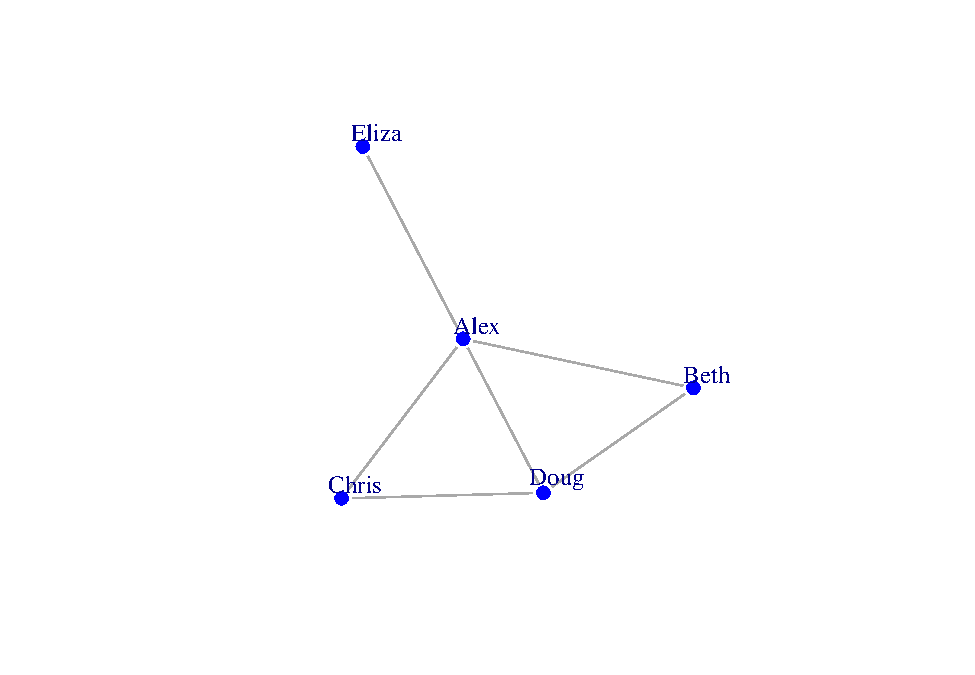
\includegraphics{bookdown-demo_files/figure-latex/unnamed-chunk-73-1.pdf}

All of the information associated with the connectivity structure of these 5 people can be represented in two ways: in an \emph{edge list} or an \emph{adjacency matrix}. The following sections will demonstrate what data in an edge list and adjacency matrix looks like, and how to import the data into RStudio so that it corresponds to the network representation that you want.

\section{Edge List}\label{edge-list}

An edge list is exactly what it says it is. A list of edges (connections) in the network. Below you can see that each edge is represented on a separate row and the name of each node in the relationship is listed in separate columns.

\begin{table}
\centering
\begin{tabular}{l|l}
\hline
Alex & Beth\\
\hline
Alex & Chris\\
\hline
Alex & Doug\\
\hline
Alex & Eliza\\
\hline
Beth & Doug\\
\hline
Chris & Doug\\
\hline
\end{tabular}
\end{table}

Specifically, an edge list refers to a type of network data representation where each row represents a single edge in the network with at least 2 columns where the labels of connected nodes are provided. The number of rows in the edge list corresponds to the number of edges in the network. Additional columns can be specified that provide more information about the edges (e.g., type, weight). These become additional ``edge attributes'' of the network.

\section{Adjacency Matrix}\label{adjacency-matrix}

An adjacency matrix refers to a type of network data representation known as an adjacency matrix where the edge connectivity is represented in the matrix. The number of rows and columns correspond to the number of nodes in the network. A non-zero value in the {[}i,j{]} element of the adjacency matrix indicates the presence of a link between node i and node j.

So in this case, the matrix has 5 rows and 5 columns (a square 5 x 5 matrix). The rows and columns are labelled with the node names. The cell carries a value of 1 if two people are connected, 0 if not connected. In this example, if we look at the first row, we can easily tell that Alex is the social butterfly of the group; he's friends with everyone in the network!

\begin{table}
\centering
\begin{tabular}{l|r|r|r|r|r}
\hline
  & Alex & Beth & Chris & Doug & Eliza\\
\hline
Alex & 0 & 1 & 1 & 1 & 1\\
\hline
Beth & 1 & 0 & 0 & 1 & 0\\
\hline
Chris & 1 & 0 & 0 & 1 & 0\\
\hline
Doug & 1 & 1 & 1 & 0 & 0\\
\hline
Eliza & 1 & 0 & 0 & 0 & 0\\
\hline
\end{tabular}
\end{table}

\begin{quote}
Eagle-eyed readers will realize that this matrix is symmetrical! This means that if you slice the matrix on its diagonal starting from the top left to the bottom right, the positions of filled cells are mirrored on the other side. This makes sense if we assume that the friendship of Alex and Beth goes both ways (Alex considers Beth a friend and Beth considers Alex a friend). In network science terms, we say that there is an undirected edge between Alex and Beth. We'll get into the nitty gritty about the different types of edges a network could have later on.
\end{quote}

\section{Importing your data and converting into a network}\label{importing-your-data-and-converting-into-a-network}

After reading the previous section, you should be able to identify whether your data set takes the form of an edge list or adjacency matrix, and if not, take the necessary steps to convert the data into one of these two formats. Depending whether it is an edge list or adjacency matrix, we will make use of different functions to convert the connectivity information into an \texttt{igraph} network object so that we can start to analyze it further.

Another point to note is that you as the modeler will have to make decisions about the type of edges your network will have. Should the edges be undirected or directed, and/or unweighted or weighted? While there are no objectively right or wrong decisions, there are probably better or worse decisions that would depend mostly on your own research questions, interpretation of the data set, and the extant network science literature on similar topics.

A final point to note is that I have created sample .csv files based on the famous Zachary Karate Club network for demonstrating the code below. All supplementary data can be obtained from Github (\url{https://github.com/csqsiew/csqsiew.github.io/tree/main/data}), and are stored in a subdirectory called \texttt{/data} from which I am reading from. Based on chapter 2 (finding files) you should be able to make the corresponding modifications to the \texttt{read.csv()} parts of the code.

\subsection{Importing edge lists}\label{importing-edge-lists}

A. You want a network with \emph{undirected, unweighted} edges.

\begin{Shaded}
\begin{Highlighting}[]
\NormalTok{karate\_el }\OtherTok{\textless{}{-}} \FunctionTok{read.csv}\NormalTok{(}\StringTok{\textquotesingle{}data/karate\_el.csv\textquotesingle{}}\NormalTok{, }\AttributeTok{header =} \ConstantTok{FALSE}\NormalTok{)}

\NormalTok{karate\_uu }\OtherTok{\textless{}{-}} \FunctionTok{graph\_from\_data\_frame}\NormalTok{(karate\_el, }\AttributeTok{directed =} \ConstantTok{FALSE}\NormalTok{)}

\FunctionTok{summary}\NormalTok{(karate\_uu)}
\end{Highlighting}
\end{Shaded}

\begin{verbatim}
## IGRAPH 372404e UN-- 34 78 -- 
## + attr: name (v/c)
\end{verbatim}

Things to note:

\begin{enumerate}
\def\labelenumi{\arabic{enumi}.}
\tightlist
\item
  \texttt{header\ =\ FALSE} in the first line - this is because there are no column headers in the \texttt{karate\_el.csv} file! You can inspect and verify this for yourself.
\item
  \texttt{directed\ =\ FALSE} in the second line - this tells R that the edges are to be interpreted as undirected.
\item
  \texttt{graph\_from\_data\_frame} is the function you would use for edge lists, which have been imported into RStudio as a data frame object.
\end{enumerate}

B. You want a network with \emph{directed, unweighted} edges.

\begin{Shaded}
\begin{Highlighting}[]
\NormalTok{karate\_el }\OtherTok{\textless{}{-}} \FunctionTok{read.csv}\NormalTok{(}\StringTok{\textquotesingle{}data/karate\_el.csv\textquotesingle{}}\NormalTok{, }\AttributeTok{header =} \ConstantTok{FALSE}\NormalTok{)}

\NormalTok{karate\_du }\OtherTok{\textless{}{-}} \FunctionTok{graph\_from\_data\_frame}\NormalTok{(karate\_el, }\AttributeTok{directed =} \ConstantTok{TRUE}\NormalTok{)}

\FunctionTok{summary}\NormalTok{(karate\_du)}
\end{Highlighting}
\end{Shaded}

\begin{verbatim}
## IGRAPH 6f42e05 DN-- 34 78 -- 
## + attr: name (v/c)
\end{verbatim}

Things to note:

\begin{enumerate}
\def\labelenumi{\arabic{enumi}.}
\tightlist
\item
  \texttt{directed\ =\ TRUE} in the second line - this tells R that the edges are to be interpreted as directed. The direction of the edges runs from the nodes in the first column of the edge list to the nodes in the second column of the edge list.
\end{enumerate}

C. You want a network with \emph{undirected, weighted} edges.

\begin{Shaded}
\begin{Highlighting}[]
\NormalTok{karate\_el }\OtherTok{\textless{}{-}} \FunctionTok{read.csv}\NormalTok{(}\StringTok{\textquotesingle{}data/karate\_el\_weights.csv\textquotesingle{}}\NormalTok{, }\AttributeTok{header =} \ConstantTok{TRUE}\NormalTok{)}

\NormalTok{karate\_uw }\OtherTok{\textless{}{-}} \FunctionTok{graph\_from\_data\_frame}\NormalTok{(karate\_el, }\AttributeTok{directed =} \ConstantTok{FALSE}\NormalTok{)}

\FunctionTok{summary}\NormalTok{(karate\_uw)}
\end{Highlighting}
\end{Shaded}

\begin{verbatim}
## IGRAPH 24ba2bd UNW- 34 78 -- 
## + attr: name (v/c), weight (e/n)
\end{verbatim}

Things to note:

\begin{enumerate}
\def\labelenumi{\arabic{enumi}.}
\tightlist
\item
  A different file is used: \texttt{karate\_el\_weights.csv}. Open the file and see for yourself that there is an additional column called \texttt{weight}. We can consider this to be a representation of the strength of relationship between two karate club members. Additional columns in an edge list are interpreted as edge attributes - see if you can spot it in the summary output of \texttt{karate\_uw}.
\item
  \texttt{header\ =\ TRUE} in the first line - this is because there \emph{are} column headers in the \texttt{karate\_el\_weights.csv} file!
\end{enumerate}

D. You want a network with \emph{directed, weighted} edges.

\begin{Shaded}
\begin{Highlighting}[]
\NormalTok{karate\_el }\OtherTok{\textless{}{-}} \FunctionTok{read.csv}\NormalTok{(}\StringTok{\textquotesingle{}data/karate\_el\_weights.csv\textquotesingle{}}\NormalTok{, }\AttributeTok{header =} \ConstantTok{TRUE}\NormalTok{)}

\NormalTok{karate\_dw }\OtherTok{\textless{}{-}} \FunctionTok{graph\_from\_data\_frame}\NormalTok{(karate\_el, }\AttributeTok{directed =} \ConstantTok{TRUE}\NormalTok{)}

\FunctionTok{summary}\NormalTok{(karate\_dw)}
\end{Highlighting}
\end{Shaded}

\begin{verbatim}
## IGRAPH bbe89b6 DNW- 34 78 -- 
## + attr: name (v/c), weight (e/n)
\end{verbatim}

\subsection{Importing adjacency matrices}\label{importing-adjacency-matrices}

A. You want a network with \emph{undirected, unweighted} edges.

\begin{Shaded}
\begin{Highlighting}[]
\NormalTok{karate\_am }\OtherTok{\textless{}{-}} \FunctionTok{read.csv}\NormalTok{(}\StringTok{\textquotesingle{}data/karate\_adj.csv\textquotesingle{}}\NormalTok{, }\AttributeTok{header =} \ConstantTok{TRUE}\NormalTok{, }\AttributeTok{row.names =} \DecValTok{1}\NormalTok{)}

\NormalTok{karate\_am }\OtherTok{\textless{}{-}} \FunctionTok{as.matrix}\NormalTok{(karate\_am) }\CommentTok{\# converts dataframe into a matrix object}

\FunctionTok{isSymmetric}\NormalTok{(karate\_am) }\CommentTok{\# sanity check that the matrix is symmetric }
\end{Highlighting}
\end{Shaded}

\begin{verbatim}
## [1] TRUE
\end{verbatim}

\begin{Shaded}
\begin{Highlighting}[]
\NormalTok{karate\_uu }\OtherTok{\textless{}{-}} \FunctionTok{graph\_from\_adjacency\_matrix}\NormalTok{(karate\_am, }\AttributeTok{mode =} \StringTok{\textquotesingle{}undirected\textquotesingle{}}\NormalTok{)}

\FunctionTok{summary}\NormalTok{(karate\_uu)}
\end{Highlighting}
\end{Shaded}

\begin{verbatim}
## IGRAPH b81ea0e UN-- 34 78 -- 
## + attr: name (v/c)
\end{verbatim}

Things to note:

\begin{enumerate}
\def\labelenumi{\arabic{enumi}.}
\tightlist
\item
  The arguments \texttt{header\ =\ TRUE} and \texttt{row.names\ =\ 1} in the \texttt{read.csv} function specify that there are column headers and row names in the first column of the dataset. Notice that the column and row labels (which correspond to the node names) are identical across both in \texttt{karate\_adj.csv}.
\item
  We need to use the function \texttt{as.matrix} to convert the dataframe object into a matrix object, since the \texttt{graph\_from\_adjacency\_matrix} expects a matrix object.
\item
  I included a sanity check - using \texttt{isSymmetric} to check if the matrix is symmetric down the diagonal. This is good to do because when creating an undirected network from an adjacency matrix, \texttt{graph\_from\_adjacency\_matrix} expects a symmetric matrix, and returns a warning message if this is not true.
\item
  Notice that we need to use a different function, \texttt{graph\_from\_adjacency\_matrix}, for converting the matrix into a network.
\end{enumerate}

B. You want a network with \emph{directed, unweighted} edges.

\begin{Shaded}
\begin{Highlighting}[]
\NormalTok{karate\_am }\OtherTok{\textless{}{-}} \FunctionTok{read.csv}\NormalTok{(}\StringTok{\textquotesingle{}data/karate\_adj.csv\textquotesingle{}}\NormalTok{, }\AttributeTok{header =} \ConstantTok{TRUE}\NormalTok{, }\AttributeTok{row.names =} \DecValTok{1}\NormalTok{)}

\NormalTok{karate\_am }\OtherTok{\textless{}{-}} \FunctionTok{as.matrix}\NormalTok{(karate\_am) }\CommentTok{\# converts dataframe into a matrix object}

\FunctionTok{isSymmetric}\NormalTok{(karate\_am) }\CommentTok{\# sanity check that the matrix is symmetric }
\end{Highlighting}
\end{Shaded}

\begin{verbatim}
## [1] TRUE
\end{verbatim}

\begin{Shaded}
\begin{Highlighting}[]
\NormalTok{karate\_du }\OtherTok{\textless{}{-}} \FunctionTok{graph\_from\_adjacency\_matrix}\NormalTok{(karate\_am, }\AttributeTok{mode =} \StringTok{\textquotesingle{}directed\textquotesingle{}}\NormalTok{)}

\FunctionTok{summary}\NormalTok{(karate\_du)}
\end{Highlighting}
\end{Shaded}

\begin{verbatim}
## IGRAPH c2d6f07 DN-- 34 156 -- 
## + attr: name (v/c)
\end{verbatim}

Things to note:

\begin{enumerate}
\def\labelenumi{\arabic{enumi}.}
\tightlist
\item
  \texttt{directed\ =\ TRUE} in the \texttt{graph\_from\_adjacency\_matrix} function - this tells R that the edges are to be interpreted as directed. For each non-empty cell in the matrix, the direction of that edge would be \textbf{from} the node in the \textbf{row}, \emph{to} the node in the \emph{column}. See figure below for a depiction.
\item
  Because of this directedness interpretation, and given that the matrix is symmetric, this implies that the network's edges are ``double counted''. A directed connection from node A to B is counted separately from the directed connection from node B to A. You can see that the number of edges in the \texttt{summary} output of this network is twice that of the previous network.
\end{enumerate}

C. You want a network with \emph{undirected, weighted} edges.

\begin{Shaded}
\begin{Highlighting}[]
\NormalTok{karate\_am }\OtherTok{\textless{}{-}} \FunctionTok{read.csv}\NormalTok{(}\StringTok{\textquotesingle{}data/karate\_adj\_weights.csv\textquotesingle{}}\NormalTok{, }\AttributeTok{header =} \ConstantTok{TRUE}\NormalTok{, }\AttributeTok{row.names =} \DecValTok{1}\NormalTok{)}

\NormalTok{karate\_am }\OtherTok{\textless{}{-}} \FunctionTok{as.matrix}\NormalTok{(karate\_am) }\CommentTok{\# converts dataframe into a matrix object}

\FunctionTok{isSymmetric}\NormalTok{(karate\_am) }\CommentTok{\# sanity check that the matrix is symmetric }
\end{Highlighting}
\end{Shaded}

\begin{verbatim}
## [1] FALSE
\end{verbatim}

\begin{Shaded}
\begin{Highlighting}[]
\NormalTok{karate\_uw }\OtherTok{\textless{}{-}} \FunctionTok{graph\_from\_adjacency\_matrix}\NormalTok{(karate\_am, }\AttributeTok{mode =} \StringTok{\textquotesingle{}undirected\textquotesingle{}}\NormalTok{, }\AttributeTok{weighted =} \StringTok{\textquotesingle{}weight\textquotesingle{}}\NormalTok{)}
\end{Highlighting}
\end{Shaded}

\begin{verbatim}
## Warning: The `adjmatrix` argument of `graph_from_adjacency_matrix()` must be symmetric with mode = "undirected" as of igraph 1.6.0.
## i Use mode = "max" to achieve the original behavior.
## This warning is displayed once every 8 hours.
## Call `lifecycle::last_lifecycle_warnings()` to see where this warning was generated.
\end{verbatim}

\begin{Shaded}
\begin{Highlighting}[]
\FunctionTok{summary}\NormalTok{(karate\_uw)}
\end{Highlighting}
\end{Shaded}

\begin{verbatim}
## IGRAPH 94bf759 UNW- 34 100 -- 
## + attr: name (v/c), weight (e/n)
\end{verbatim}

Things to note:

\begin{enumerate}
\def\labelenumi{\arabic{enumi}.}
\tightlist
\item
  See if you can tell how \texttt{karate\_adj\_weights.csv} is different from \texttt{karate\_adj.csv}. The numbers in the cells for the former file can take on values other than 0s and 1s. This is typically used to depict the weight of the connection between two nodes.
\item
  \texttt{weighted\ =\ \textquotesingle{}weight\textquotesingle{}} informs \texttt{igraph} that the values in the cell (which range from 1 to 5) are to be assigned as values of an edge attribute called \texttt{\textquotesingle{}weight\textquotesingle{}}. This is how you get a network with weighted edges.
\end{enumerate}

D. You want a network with \emph{directed, weighted} edges

\begin{Shaded}
\begin{Highlighting}[]
\NormalTok{karate\_am }\OtherTok{\textless{}{-}} \FunctionTok{read.csv}\NormalTok{(}\StringTok{\textquotesingle{}data/karate\_adj\_weights.csv\textquotesingle{}}\NormalTok{, }\AttributeTok{header =} \ConstantTok{TRUE}\NormalTok{, }\AttributeTok{row.names =} \DecValTok{1}\NormalTok{)}

\NormalTok{karate\_am }\OtherTok{\textless{}{-}} \FunctionTok{as.matrix}\NormalTok{(karate\_am) }\CommentTok{\# converts dataframe into a matrix object}

\FunctionTok{isSymmetric}\NormalTok{(karate\_am) }\CommentTok{\# sanity check that the matrix is symmetric }
\end{Highlighting}
\end{Shaded}

\begin{verbatim}
## [1] FALSE
\end{verbatim}

\begin{Shaded}
\begin{Highlighting}[]
\NormalTok{karate\_dw }\OtherTok{\textless{}{-}} \FunctionTok{graph\_from\_adjacency\_matrix}\NormalTok{(karate\_am, }\AttributeTok{mode =} \StringTok{\textquotesingle{}directed\textquotesingle{}}\NormalTok{, }\AttributeTok{weighted =} \StringTok{\textquotesingle{}weight\textquotesingle{}}\NormalTok{)}

\FunctionTok{summary}\NormalTok{(karate\_dw)}
\end{Highlighting}
\end{Shaded}

\begin{verbatim}
## IGRAPH 8b4b333 DNW- 34 103 -- 
## + attr: name (v/c), weight (e/n)
\end{verbatim}

\section{Exercise}\label{exercise-3}

Janelle is interested in modeling the social network structure of her cats. In order to construct the network, she observed the interaction patterns of her cats for a week. Here are her observations:

\begin{enumerate}
\def\labelenumi{\arabic{enumi}.}
\tightlist
\item
  Niko and Russell seem to get on quite well. Niko likes to eat Russell's food.
\item
  Annabelle and Sammy were adopted at the same time and tend to stick close to each other.
\item
  Janelle noticed that Jo has been napping next to Jack in the study room.
\item
  Sammy, Russell, and Groucho love playing with the ball of twine in the living room.
\item
  Groucho and Russell are elderly cats who seem to have a mutual respect for each other.
\item
  The only cat that Dottie is able to tolerate is Niko.
\end{enumerate}

Your task is to:

\begin{enumerate}
\def\labelenumi{(\roman{enumi})}
\tightlist
\item
  create the raw data file for this network (a .csv file)
\item
  convert the data into a network object in igraph
\item
  visualize the network using \texttt{plot(network\_name)}
\item
  print the output of the network object
\item
  save your network object as a .RData (and see if you are able to reload it into RStudio)
\end{enumerate}

\chapter{Chapter 5: Manipulating network objects}\label{ch5}

In this chapter we explore how network objects can be ``manipulated'' based on their node or edge attributes. This can be especially useful if you wish to segment or subset your network so that you can analyze networks of different types. For instance, you may wish to explore how your network analysis results change depending on the threshold used to remove edges of varying weights (edge attribute). Another example could be that you are only interested in analyzing language networks where the nodes represent nouns, and not other parts of speech like verbs or adjectives (node attribute). We will also learn how to add these node and edge attributes to the network.

\section{Set up}\label{set-up}

We will use the \texttt{karate} network as our example in this chapter.

\begin{Shaded}
\begin{Highlighting}[]
\FunctionTok{library}\NormalTok{(igraph)}
\FunctionTok{library}\NormalTok{(igraphdata)}
\FunctionTok{library}\NormalTok{(tidyverse)}

\FunctionTok{data}\NormalTok{(}\StringTok{\textquotesingle{}karate\textquotesingle{}}\NormalTok{)}

\FunctionTok{summary}\NormalTok{(karate)}
\end{Highlighting}
\end{Shaded}

\begin{verbatim}
## This graph was created by an old(er) igraph version.
##   Call upgrade_graph() on it to use with the current igraph version
##   For now we convert it on the fly...
\end{verbatim}

\begin{verbatim}
## IGRAPH 4b458a1 UNW- 34 78 -- Zachary's karate club network
## + attr: name (g/c), Citation (g/c), Author (g/c), Faction (v/n), name (v/c), label (v/c), color (v/n), weight (e/n)
\end{verbatim}

\section{Adding node attributes}\label{adding-node-attributes}

An important feature of psychological networks is that we are usually interested in more than just the underlying mathematics of the network, but rather we want to know how these network measures relate to behavior. This implies that the nodes in psychological networks are typically associated with rich psychological variables. For instance, nodes depicting individuals of different ages and genders, or nodes depicting words with different values on lexical-semantic variables like valence and arousal.

We need to add this node information as node attributes to the network representation.

In the code below, we output the list of nodes so that we can merge this data frame to the node attributes (can be done external to RStudio or internally within RStudio using data wrangling methods). This is because node attributes are additional variables that you have knowledge of or have collected in your study.

\begin{Shaded}
\begin{Highlighting}[]
\CommentTok{\# export your node names, enter attributes manually outside of R }
\FunctionTok{write.csv}\NormalTok{(}\FunctionTok{data.frame}\NormalTok{(}\AttributeTok{node =} \FunctionTok{V}\NormalTok{(karate)}\SpecialCharTok{$}\NormalTok{name), }\AttributeTok{file =} \StringTok{\textquotesingle{}karate\_nodes.csv\textquotesingle{}}\NormalTok{, }\AttributeTok{row.names =}\NormalTok{ F)}
\end{Highlighting}
\end{Shaded}

In the \texttt{karate\_node\_added.csv} file, sample node attributes for the \texttt{karate} network have been added. The code below shows you how to read in this data and add this information as node attributes to the network using the \texttt{set\_vertex\_attribute} function.

\begin{Shaded}
\begin{Highlighting}[]
\CommentTok{\# import your node attributes }
\NormalTok{node\_info }\OtherTok{\textless{}{-}} \FunctionTok{read.csv}\NormalTok{(}\StringTok{\textquotesingle{}data/karate\_nodes\_added.csv\textquotesingle{}}\NormalTok{, }\AttributeTok{header =}\NormalTok{ T)}

\CommentTok{\# very important to ensure that node order is identical }
\NormalTok{node\_info }\OtherTok{\textless{}{-}}\NormalTok{ node\_info }\SpecialCharTok{\%\textgreater{}\%} \FunctionTok{arrange}\NormalTok{(}\FunctionTok{factor}\NormalTok{(node, }\AttributeTok{levels =} \FunctionTok{V}\NormalTok{(karate)}\SpecialCharTok{$}\NormalTok{name))}

\FunctionTok{identical}\NormalTok{(}\FunctionTok{V}\NormalTok{(karate)}\SpecialCharTok{$}\NormalTok{name, node\_info}\SpecialCharTok{$}\NormalTok{node) }\CommentTok{\# sanity check that the node name order is identical}
\end{Highlighting}
\end{Shaded}

\begin{verbatim}
## [1] TRUE
\end{verbatim}

\begin{Shaded}
\begin{Highlighting}[]
\CommentTok{\# add the \textquotesingle{}gender\textquotesingle{} attribute}
\NormalTok{karate }\OtherTok{\textless{}{-}} \FunctionTok{set\_vertex\_attr}\NormalTok{(karate, }
                          \AttributeTok{name =} \StringTok{\textquotesingle{}gender\textquotesingle{}}\NormalTok{,}
                          \AttributeTok{value =}\NormalTok{ node\_info}\SpecialCharTok{$}\NormalTok{gender)}

\CommentTok{\# add the \textquotesingle{}belt\textquotesingle{} attribute}
\NormalTok{karate }\OtherTok{\textless{}{-}} \FunctionTok{set\_vertex\_attr}\NormalTok{(karate, }
                          \AttributeTok{name =} \StringTok{\textquotesingle{}belt\textquotesingle{}}\NormalTok{,}
                          \AttributeTok{value =}\NormalTok{ node\_info}\SpecialCharTok{$}\NormalTok{belt)}

\CommentTok{\# add the \textquotesingle{}age\textquotesingle{} attribute }
\NormalTok{karate }\OtherTok{\textless{}{-}} \FunctionTok{set\_vertex\_attr}\NormalTok{(karate, }
                          \AttributeTok{name =} \StringTok{\textquotesingle{}age\textquotesingle{}}\NormalTok{,}
                          \AttributeTok{value =}\NormalTok{ node\_info}\SpecialCharTok{$}\NormalTok{age)}

\FunctionTok{summary}\NormalTok{(karate) }\CommentTok{\# these vertex attributes should show up in the summary}
\end{Highlighting}
\end{Shaded}

\begin{verbatim}
## IGRAPH 4b458a1 UNW- 34 78 -- Zachary's karate club network
## + attr: name (g/c), Citation (g/c), Author (g/c), Faction (v/n), name (v/c), label (v/c), color (v/n), gender (v/c), belt (v/c), age (v/n), weight (e/n)
\end{verbatim}

A key point is to ensure that the node ordering in your .csv file is identical to that of the network - this can be assured using the \texttt{arrange} function from \texttt{tidyverse}. This is to ensure accurate mapping from your data frame to the network.

When you run \texttt{summary(karate)} hopefully you will see that there are additional labels (gender, belt, age) included in the attributes section.

\section{Adding edge attributes}\label{adding-edge-attributes}

Because there are usually more edges than nodes in the network, we usually do not manually insert edge attributes by hand (although it is possible!). In Chapter 4 recall that edge weights are usually included in the network at the point of network construction, as edge weights are in an additional column in the edge list that you are importing into RStudio.

Here we explore a simple case where you want to ``tag'' and color edges differently depending on whether the tie is between \emph{same} or \emph{different} genders.

\begin{Shaded}
\begin{Highlighting}[]
\CommentTok{\# initialize all edges with the same label }
\FunctionTok{E}\NormalTok{(karate)}\SpecialCharTok{$}\NormalTok{edge\_type }\OtherTok{\textless{}{-}} \StringTok{\textquotesingle{}same\textquotesingle{}} 

\CommentTok{\# re{-}assign those with mixed edges to a new label }
\FunctionTok{E}\NormalTok{(karate)}\SpecialCharTok{$}\NormalTok{edge\_type[}\FunctionTok{E}\NormalTok{(karate)[}\FunctionTok{V}\NormalTok{(karate)[}\FunctionTok{V}\NormalTok{(karate)}\SpecialCharTok{$}\NormalTok{gender }\SpecialCharTok{==} \StringTok{\textquotesingle{}male\textquotesingle{}}\NormalTok{] }\SpecialCharTok{\%{-}{-}\%} \FunctionTok{V}\NormalTok{(karate)[}\FunctionTok{V}\NormalTok{(karate)}\SpecialCharTok{$}\NormalTok{gender }\SpecialCharTok{==} \StringTok{\textquotesingle{}female\textquotesingle{}}\NormalTok{]]] }\OtherTok{\textless{}{-}} \StringTok{\textquotesingle{}different\textquotesingle{}}

\FunctionTok{summary}\NormalTok{(karate) }\CommentTok{\# there should be a new edge type }
\end{Highlighting}
\end{Shaded}

\begin{verbatim}
## IGRAPH 4b458a1 UNW- 34 78 -- Zachary's karate club network
## + attr: name (g/c), Citation (g/c), Author (g/c), Faction (v/n), name (v/c), label (v/c), color (v/n), gender (v/c), belt (v/c), age (v/n), weight (e/n), edge_type (e/c)
\end{verbatim}

\begin{Shaded}
\begin{Highlighting}[]
\FunctionTok{E}\NormalTok{(karate)}\SpecialCharTok{$}\NormalTok{edge\_type}
\end{Highlighting}
\end{Shaded}

\begin{verbatim}
##  [1] "same"      "same"      "same"      "same"      "different" "same"      "same"      "same"      "same"      "different" "different" "same"      "different" "same"      "same"      "different" "same"     
## [18] "same"      "same"      "same"      "different" "same"      "same"      "same"      "same"      "same"      "same"      "same"      "same"      "different" "same"      "different" "same"      "different"
## [35] "same"      "same"      "same"      "different" "different" "same"      "different" "same"      "different" "same"      "same"      "same"      "same"      "different" "same"      "different" "different"
## [52] "same"      "same"      "different" "same"      "different" "same"      "same"      "different" "different" "different" "same"      "same"      "different" "different" "different" "same"      "different"
## [69] "different" "different" "same"      "same"      "different" "different" "same"      "same"      "different" "different"
\end{verbatim}

\begin{Shaded}
\begin{Highlighting}[]
\CommentTok{\# this tells you the ordering of the levels so you can tell that red = different and blue = same }
\FunctionTok{factor}\NormalTok{(}\FunctionTok{E}\NormalTok{(karate)}\SpecialCharTok{$}\NormalTok{edge\_type) }\SpecialCharTok{|\textgreater{}} \FunctionTok{levels}\NormalTok{()}
\end{Highlighting}
\end{Shaded}

\begin{verbatim}
## [1] "different" "same"
\end{verbatim}

We can then easily visualize the different edge types in the network.

\begin{Shaded}
\begin{Highlighting}[]
\CommentTok{\# note the use of factor()}
\FunctionTok{plot}\NormalTok{(karate, }\AttributeTok{vertex.color =} \StringTok{\textquotesingle{}white\textquotesingle{}}\NormalTok{, }\AttributeTok{edge.color =} \FunctionTok{factor}\NormalTok{(}\FunctionTok{E}\NormalTok{(karate)}\SpecialCharTok{$}\NormalTok{edge\_type))}
\end{Highlighting}
\end{Shaded}

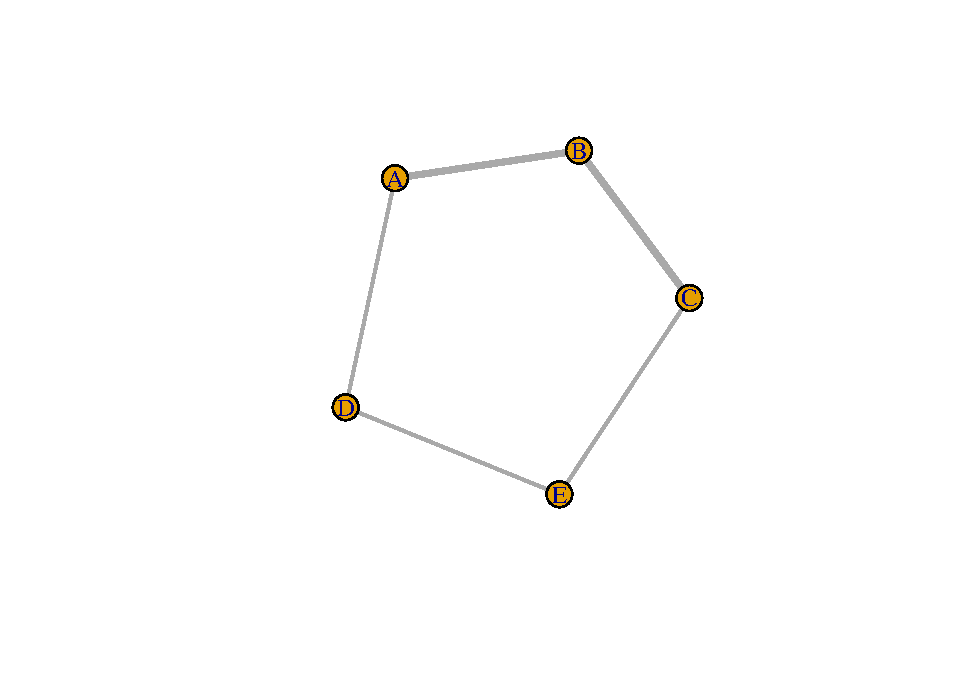
\includegraphics{bookdown-demo_files/figure-latex/unnamed-chunk-88-1.pdf}

\begin{Shaded}
\begin{Highlighting}[]
\CommentTok{\# specifying your own colors }
\FunctionTok{plot}\NormalTok{(karate, }\AttributeTok{vertex.color =} \StringTok{\textquotesingle{}white\textquotesingle{}}\NormalTok{, }\AttributeTok{edge.color =} \FunctionTok{c}\NormalTok{(}\StringTok{\textquotesingle{}red\textquotesingle{}}\NormalTok{, }\StringTok{\textquotesingle{}blue\textquotesingle{}}\NormalTok{)[}\FunctionTok{factor}\NormalTok{(}\FunctionTok{E}\NormalTok{(karate)}\SpecialCharTok{$}\NormalTok{edge\_type)])}
\end{Highlighting}
\end{Shaded}

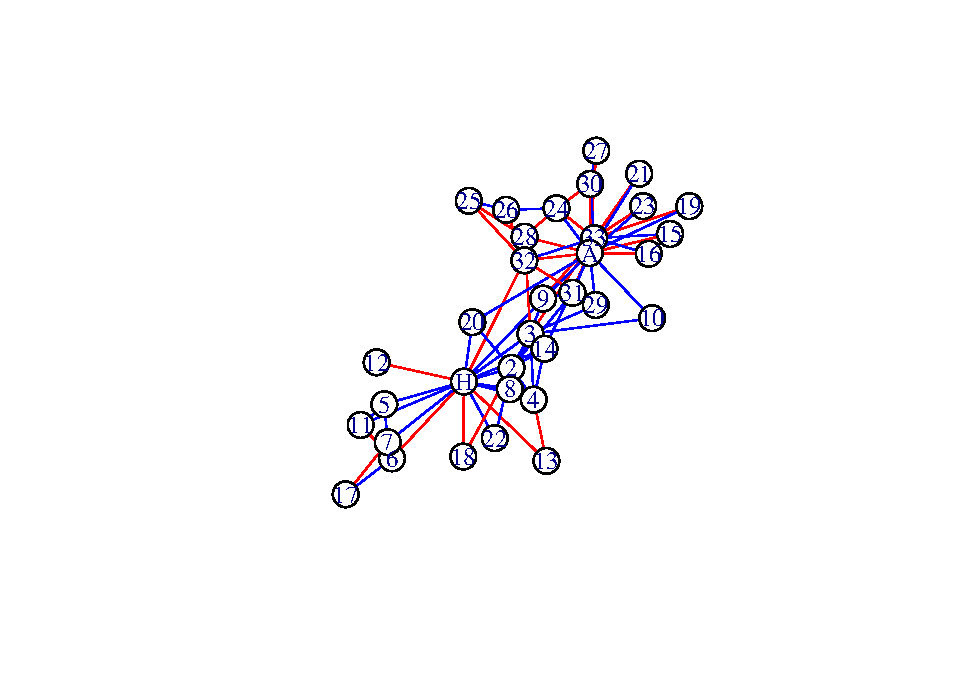
\includegraphics{bookdown-demo_files/figure-latex/unnamed-chunk-88-2.pdf}

\section{Subsetting the network}\label{subsetting-the-network}

\subsection{Subset by node attributes}\label{subset-by-node-attributes}

The example below subsets the \texttt{karate} networks to only retain male individuals.

\begin{Shaded}
\begin{Highlighting}[]
\NormalTok{karate\_male }\OtherTok{\textless{}{-}} \FunctionTok{induced\_subgraph}\NormalTok{(}\AttributeTok{graph =}\NormalTok{ karate,}
                                \AttributeTok{vids =} \FunctionTok{V}\NormalTok{(karate)}\SpecialCharTok{$}\NormalTok{gender }\SpecialCharTok{==} \StringTok{\textquotesingle{}female\textquotesingle{}}\NormalTok{)}

\FunctionTok{summary}\NormalTok{(karate\_male)}
\end{Highlighting}
\end{Shaded}

\begin{verbatim}
## IGRAPH 8946ba7 UNW- 12 6 -- Zachary's karate club network
## + attr: name (g/c), Citation (g/c), Author (g/c), Faction (v/n), name (v/c), label (v/c), color (v/n), gender (v/c), belt (v/c), age (v/n), weight (e/n), edge_type (e/c)
\end{verbatim}

How would you change the code to retain female individuals?

\subsection{Subset by a target node}\label{subset-by-a-target-node}

The example below shows you how to extract the immediate neighborhood structure of a particular node (the ego).

\begin{Shaded}
\begin{Highlighting}[]
\NormalTok{mrhi }\OtherTok{\textless{}{-}} \FunctionTok{make\_ego\_graph}\NormalTok{(karate, }\AttributeTok{order =} \DecValTok{1}\NormalTok{, }\AttributeTok{nodes =} \StringTok{\textquotesingle{}Actor 2\textquotesingle{}}\NormalTok{)[[}\DecValTok{1}\NormalTok{]] }\CommentTok{\# order = 1 (immediate neighbors)}

\FunctionTok{summary}\NormalTok{(mrhi)}
\end{Highlighting}
\end{Shaded}

\begin{verbatim}
## IGRAPH 30d3270 UNW- 10 21 -- Zachary's karate club network
## + attr: name (g/c), Citation (g/c), Author (g/c), Faction (v/n), name (v/c), label (v/c), color (v/n), gender (v/c), belt (v/c), age (v/n), weight (e/n), edge_type (e/c)
\end{verbatim}

\begin{Shaded}
\begin{Highlighting}[]
\FunctionTok{plot}\NormalTok{(mrhi, }\AttributeTok{vertex.color =} \StringTok{\textquotesingle{}white\textquotesingle{}}\NormalTok{)}
\end{Highlighting}
\end{Shaded}

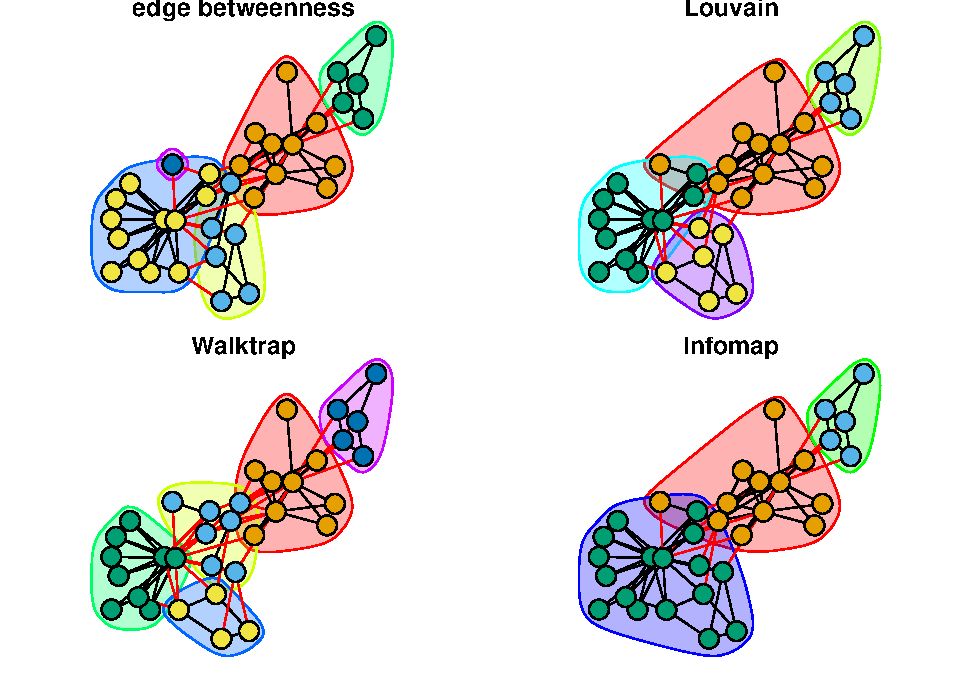
\includegraphics{bookdown-demo_files/figure-latex/unnamed-chunk-90-1.pdf}

We can also extract the ego's 2-hop neighborhood - this includes their immediate connections, and the connections of the connections. This can be easily done by changing the \texttt{order} argument.

\begin{Shaded}
\begin{Highlighting}[]
\NormalTok{mrhi2 }\OtherTok{\textless{}{-}} \FunctionTok{make\_ego\_graph}\NormalTok{(karate, }\AttributeTok{order =} \DecValTok{2}\NormalTok{, }\AttributeTok{nodes =} \StringTok{\textquotesingle{}Mr Hi\textquotesingle{}}\NormalTok{)[[}\DecValTok{1}\NormalTok{]] }\CommentTok{\# order = 2 (immediate + neighbors of neighbors)}

\FunctionTok{summary}\NormalTok{(mrhi2)}
\end{Highlighting}
\end{Shaded}

\begin{verbatim}
## IGRAPH 4f0b4d4 UNW- 26 59 -- Zachary's karate club network
## + attr: name (g/c), Citation (g/c), Author (g/c), Faction (v/n), name (v/c), label (v/c), color (v/n), gender (v/c), belt (v/c), age (v/n), weight (e/n), edge_type (e/c)
\end{verbatim}

\begin{Shaded}
\begin{Highlighting}[]
\FunctionTok{plot}\NormalTok{(mrhi2, }\AttributeTok{vertex.color =} \StringTok{\textquotesingle{}white\textquotesingle{}}\NormalTok{)}
\end{Highlighting}
\end{Shaded}

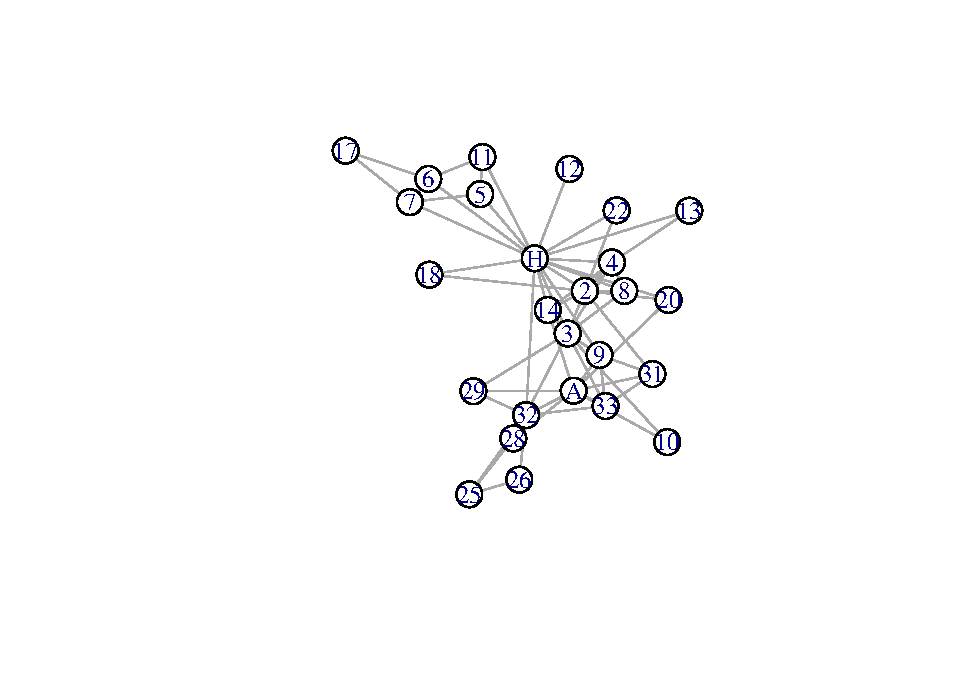
\includegraphics{bookdown-demo_files/figure-latex/unnamed-chunk-91-1.pdf}

\subsection{Subset by edge attributes}\label{subset-by-edge-attributes}

We can also subset a network by their edge attributes. Below shows an example where we only want to retain edges that between males and females (i.e., different genders).

The \texttt{eids} argument looks a bit crazy, but what it is doing to subset from all of the edges in the original network, the set of edges that connect nodes that are female and male. \texttt{\%-\/-\%} is a special \texttt{igraph} operator that looks for the edges that join two sets of specified vertices (here we are using the square operator to select nodes of various attributes). \emph{Think about what aspect of this argument you would be modify in order to retain the edges between females only.}

\begin{Shaded}
\begin{Highlighting}[]
\CommentTok{\# retain edges of the network where the connection is between a male and a female (i.e., mixed edges)}
\NormalTok{mixed\_network }\OtherTok{\textless{}{-}} \FunctionTok{subgraph.edges}\NormalTok{(}\AttributeTok{graph =}\NormalTok{ karate, }
                                \AttributeTok{eids =} \FunctionTok{E}\NormalTok{(karate)[}\FunctionTok{V}\NormalTok{(karate)[}\FunctionTok{V}\NormalTok{(karate)}\SpecialCharTok{$}\NormalTok{gender }\SpecialCharTok{==} \StringTok{\textquotesingle{}female\textquotesingle{}}\NormalTok{] }\SpecialCharTok{\%{-}{-}\%} \FunctionTok{V}\NormalTok{(karate)[}\FunctionTok{V}\NormalTok{(karate)}\SpecialCharTok{$}\NormalTok{gender }\SpecialCharTok{==} \StringTok{\textquotesingle{}male\textquotesingle{}}\NormalTok{]]}
\NormalTok{                                ) }

\CommentTok{\# eids = E(network)$weight \textgreater{} 4}

\FunctionTok{plot}\NormalTok{(mixed\_network, }\AttributeTok{vertex.color =} \FunctionTok{factor}\NormalTok{(}\FunctionTok{V}\NormalTok{(mixed\_network)}\SpecialCharTok{$}\NormalTok{gender)) }
\end{Highlighting}
\end{Shaded}

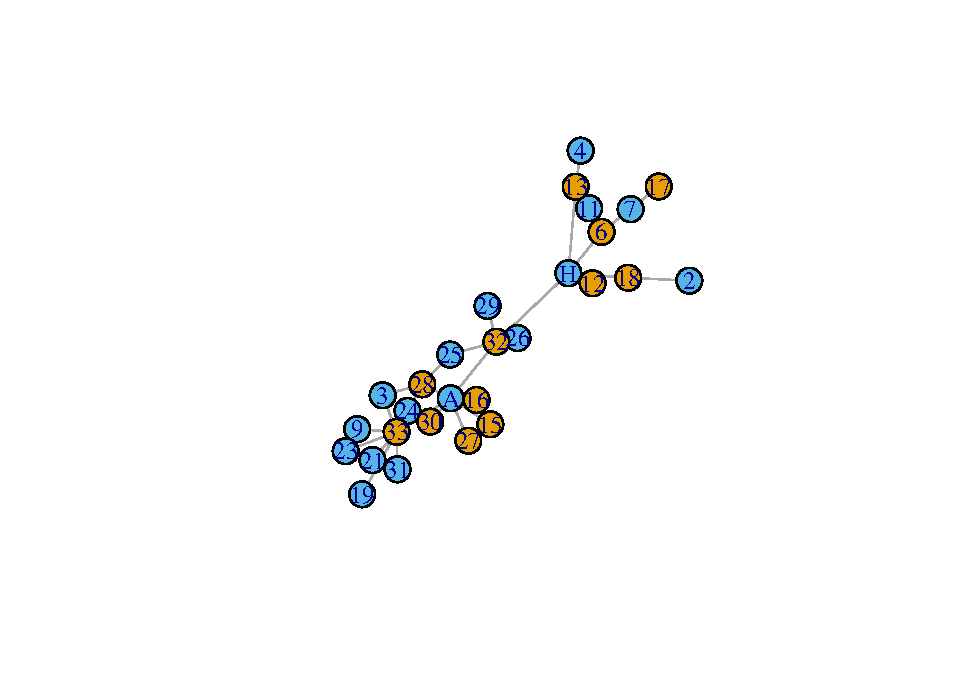
\includegraphics{bookdown-demo_files/figure-latex/unnamed-chunk-92-1.pdf}

If you have a weighted graph, it is also possible to subset the network based on edge weights. The code below retains edges that have a weight greater than 4. Play around with this argument and see if you can subset the network based on different weight thresholds. For instance, if you are interested in studying acquaintance relations, then you may decide to retain weak edges, but if you are interested in studying close relations, then you may decide to retain the strongest edges.

\begin{Shaded}
\begin{Highlighting}[]
\NormalTok{example\_network }\OtherTok{\textless{}{-}} \FunctionTok{subgraph.edges}\NormalTok{(}\AttributeTok{graph =}\NormalTok{ karate, }
                                  \AttributeTok{eids =} \FunctionTok{E}\NormalTok{(karate)[}\FunctionTok{E}\NormalTok{(karate)}\SpecialCharTok{$}\NormalTok{weight }\SpecialCharTok{\textgreater{}} \DecValTok{4}\NormalTok{]}
\NormalTok{                                  ) }

\FunctionTok{plot}\NormalTok{(example\_network)}
\end{Highlighting}
\end{Shaded}

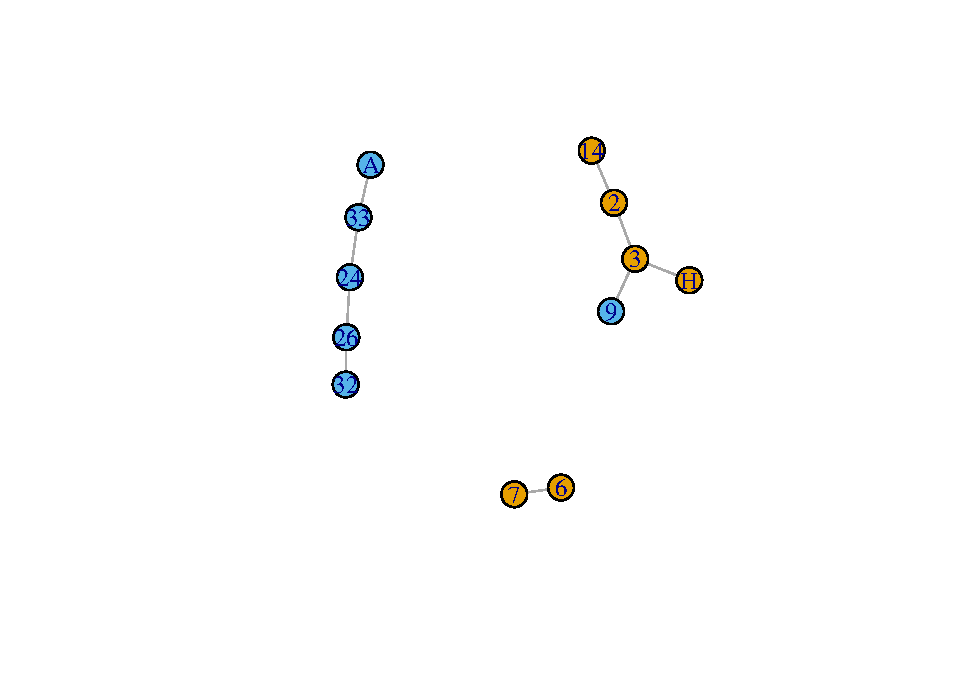
\includegraphics{bookdown-demo_files/figure-latex/unnamed-chunk-93-1.pdf}

\subsection{Subsetting by mutual edges}\label{subsetting-by-mutual-edges}

This section is most applicable for directed networks, as you may wish to subset a network based on whether edges are mutual (1--\textgreater2 AND 2--\textgreater1) or asymmetrical (1--\textgreater2 but there is no connection from 2 to 1).

To illustrate this, we first have to convert our \texttt{karate} network into a directed graph.

\begin{Shaded}
\begin{Highlighting}[]
\NormalTok{karate\_d1 }\OtherTok{\textless{}{-}} \FunctionTok{as.directed}\NormalTok{(karate, }\AttributeTok{mode =} \StringTok{\textquotesingle{}random\textquotesingle{}}\NormalTok{) }\CommentTok{\# convert undirected edges into directed edges }
\NormalTok{karate\_d2 }\OtherTok{\textless{}{-}} \FunctionTok{as.directed}\NormalTok{(karate, }\AttributeTok{mode =} \StringTok{\textquotesingle{}mutual\textquotesingle{}}\NormalTok{) }\CommentTok{\# convert undirected edges into mutual, directed edges}

\FunctionTok{summary}\NormalTok{(karate\_d1)}
\end{Highlighting}
\end{Shaded}

\begin{verbatim}
## IGRAPH c266607 DNW- 34 78 -- Zachary's karate club network
## + attr: name (g/c), Citation (g/c), Author (g/c), Faction (v/n), name (v/c), label (v/c), color (v/n), gender (v/c), belt (v/c), age (v/n), weight (e/n), edge_type (e/c)
\end{verbatim}

\begin{Shaded}
\begin{Highlighting}[]
\FunctionTok{summary}\NormalTok{(karate\_d2)}
\end{Highlighting}
\end{Shaded}

\begin{verbatim}
## IGRAPH e6b4530 DNW- 34 156 -- Zachary's karate club network
## + attr: name (g/c), Citation (g/c), Author (g/c), Faction (v/n), name (v/c), label (v/c), color (v/n), gender (v/c), belt (v/c), age (v/n), weight (e/n), edge_type (e/c)
\end{verbatim}

Notice from the summary output that \texttt{karate\_d2} has twice the number of edges than \texttt{karate\_d1}. This is because each undirected edge has been converted into two directed edges (mutual) connecting the node pair in both directions.

We can use the function \texttt{which\_mutual} to detect mutual directed edges in the network and use this to subset the network accordingly. Notice that to select for the non-mutual edges, we can use the \texttt{!} or NOT operator.

\begin{Shaded}
\begin{Highlighting}[]
\CommentTok{\# retain mutual edges }
\FunctionTok{subgraph.edges}\NormalTok{(karate\_d1, }\AttributeTok{eids =} \FunctionTok{E}\NormalTok{(karate\_d1)[}\FunctionTok{which\_mutual}\NormalTok{(karate\_d1)], }\AttributeTok{delete.vertices =} \ConstantTok{TRUE}\NormalTok{) }\SpecialCharTok{|\textgreater{}} 
  \FunctionTok{summary}\NormalTok{() }\CommentTok{\# empty graph}
\end{Highlighting}
\end{Shaded}

\begin{verbatim}
## IGRAPH e62e115 DNW- 0 0 -- Zachary's karate club network
## + attr: name (g/c), Citation (g/c), Author (g/c), Faction (v/n), name (v/c), label (v/c), color (v/n), gender (v/c), belt (v/c), age (v/n), weight (e/n), edge_type (e/c)
\end{verbatim}

\begin{Shaded}
\begin{Highlighting}[]
\FunctionTok{subgraph.edges}\NormalTok{(karate\_d2, }\AttributeTok{eids =} \FunctionTok{E}\NormalTok{(karate\_d2)[}\FunctionTok{which\_mutual}\NormalTok{(karate\_d2)], }\AttributeTok{delete.vertices =} \ConstantTok{TRUE}\NormalTok{) }\SpecialCharTok{|\textgreater{}} 
  \FunctionTok{summary}\NormalTok{()}
\end{Highlighting}
\end{Shaded}

\begin{verbatim}
## IGRAPH 6e7e930 DNW- 34 156 -- Zachary's karate club network
## + attr: name (g/c), Citation (g/c), Author (g/c), Faction (v/n), name (v/c), label (v/c), color (v/n), gender (v/c), belt (v/c), age (v/n), weight (e/n), edge_type (e/c)
\end{verbatim}

\begin{Shaded}
\begin{Highlighting}[]
\CommentTok{\# retain non{-}mutual edges }
\FunctionTok{subgraph.edges}\NormalTok{(karate\_d1, }\AttributeTok{eids =} \FunctionTok{E}\NormalTok{(karate\_d1)[}\SpecialCharTok{!}\FunctionTok{which\_mutual}\NormalTok{(karate\_d1)], }\AttributeTok{delete.vertices =} \ConstantTok{TRUE}\NormalTok{) }\SpecialCharTok{|\textgreater{}} 
  \FunctionTok{summary}\NormalTok{()}
\end{Highlighting}
\end{Shaded}

\begin{verbatim}
## IGRAPH 821ca94 DNW- 34 78 -- Zachary's karate club network
## + attr: name (g/c), Citation (g/c), Author (g/c), Faction (v/n), name (v/c), label (v/c), color (v/n), gender (v/c), belt (v/c), age (v/n), weight (e/n), edge_type (e/c)
\end{verbatim}

\begin{Shaded}
\begin{Highlighting}[]
\FunctionTok{subgraph.edges}\NormalTok{(karate\_d2, }\AttributeTok{eids =} \FunctionTok{E}\NormalTok{(karate\_d2)[}\SpecialCharTok{!}\FunctionTok{which\_mutual}\NormalTok{(karate\_d2)], }\AttributeTok{delete.vertices =} \ConstantTok{TRUE}\NormalTok{) }\SpecialCharTok{|\textgreater{}} 
  \FunctionTok{summary}\NormalTok{() }\CommentTok{\# empty graph}
\end{Highlighting}
\end{Shaded}

\begin{verbatim}
## IGRAPH c8d8682 DNW- 0 0 -- Zachary's karate club network
## + attr: name (g/c), Citation (g/c), Author (g/c), Faction (v/n), name (v/c), label (v/c), color (v/n), gender (v/c), belt (v/c), age (v/n), weight (e/n), edge_type (e/c)
\end{verbatim}

Notice from the summary output that you get different results depending on the way that the directed graph is constructed. In these toy examples, the directed edges in the network were either ALL mutual edges or ALL non-mutual edges. If you have a network with varying proportions of mutual and non-mutual edges these functions can be useful for assessing the overall mutuality of the directed graph.

\section{Useful functions}\label{useful-functions}

Finally, below are some useful functions for network manipulations that you can learn more about by reading the documentatoin.

\begin{Shaded}
\begin{Highlighting}[]
\FunctionTok{as.directed}\NormalTok{() }\CommentTok{\# convert your undirected edges to directed edges, see documentation }

\FunctionTok{as.undirected}\NormalTok{() }\CommentTok{\# convert your directed edges to undirected edges, see documentation }

\NormalTok{new\_network }\OtherTok{\textless{}{-}} \FunctionTok{remove.edge.attribute}\NormalTok{(network, }\StringTok{\textquotesingle{}weight\textquotesingle{}}\NormalTok{) }\CommentTok{\# to convert weighted to unweighted graph }
\end{Highlighting}
\end{Shaded}

\chapter{Chapter 6: Macro-level network measures}\label{ch6}

In this section, we will review network science measures that describe the overall or global structure of the entire network. You can think of these measures as providing a ``bird's eye view'' of your network, and they are useful for comparing different network representations.

To facilitate the demonstrations below, we will use the undirected, unweighted karate network that we have previously seen in Chapter 4. In the rest of the chapter we will compute various macro-level network measures for this network.

\begin{Shaded}
\begin{Highlighting}[]
\NormalTok{karate\_el }\OtherTok{\textless{}{-}} \FunctionTok{read.csv}\NormalTok{(}\StringTok{\textquotesingle{}data/karate\_el.csv\textquotesingle{}}\NormalTok{, }\AttributeTok{header =} \ConstantTok{FALSE}\NormalTok{)}

\NormalTok{karate\_uu }\OtherTok{\textless{}{-}} \FunctionTok{graph\_from\_data\_frame}\NormalTok{(karate\_el, }\AttributeTok{directed =} \ConstantTok{FALSE}\NormalTok{)}

\FunctionTok{summary}\NormalTok{(karate\_uu)}
\end{Highlighting}
\end{Shaded}

\begin{verbatim}
## IGRAPH 5f98de6 UN-- 34 78 -- 
## + attr: name (v/c)
\end{verbatim}

Although it is possible to compute macro-level network measures for directed, weighted networks in certain instances (and this will be pointed out where appropriate), I choose to focus on the undirected, unweighted version for this chapter because macro-level measures are more complex to interpret and less intuitive when additional information like edge weights and direction are included. For instance, \emph{network density} refers to the ratio of the number of (existing) edges and the number of possible edges among nodes in the network--it is not clear how this measure be adapted if we wanted to use weighted edges instead.

\section{Average Degree}\label{average-degree}

A common method of characterizing the global structure of networks is to simply compute \textbf{average degree}, which is the mean of the degree of all nodes in the network. A node's degree refers to the number of connections or edges that are incident to the node.

We first use \texttt{degree} to compute degree for each node (see Chapter 7: Degree) and then pipe the output to get the mean degree for the entire network.

\begin{Shaded}
\begin{Highlighting}[]
\FunctionTok{degree}\NormalTok{(karate\_uu) }\SpecialCharTok{|\textgreater{}} \FunctionTok{mean}\NormalTok{()}
\end{Highlighting}
\end{Shaded}

\begin{verbatim}
## [1] 4.588235
\end{verbatim}

On average, each node in the karate network has 4.5 connections.

In Chapter 7 we will learn that it is possible to compute different variants of degree for directed graphs. In-degree refers to the number of edges incoming to the target node, out-degree refers to the number of edges outgoing from to the target node, and all-degree refers to all the edges (the sum of in- and out-degree). Try running the code below on a network with directed edges.

\begin{Shaded}
\begin{Highlighting}[]
\CommentTok{\# mean in{-}degree}
\FunctionTok{degree}\NormalTok{(karate\_uu, }\AttributeTok{mode =} \StringTok{\textquotesingle{}in\textquotesingle{}}\NormalTok{) }\SpecialCharTok{|\textgreater{}} \FunctionTok{mean}\NormalTok{()}

\CommentTok{\# mean out{-}degree}
\FunctionTok{degree}\NormalTok{(karate\_uu, }\AttributeTok{mode =} \StringTok{\textquotesingle{}out\textquotesingle{}}\NormalTok{) }\SpecialCharTok{|\textgreater{}} \FunctionTok{mean}\NormalTok{()}

\CommentTok{\# mean all{-}degree}
\FunctionTok{degree}\NormalTok{(karate\_uu, }\AttributeTok{mode =} \StringTok{\textquotesingle{}all\textquotesingle{}}\NormalTok{) }\SpecialCharTok{|\textgreater{}} \FunctionTok{mean}\NormalTok{()}
\end{Highlighting}
\end{Shaded}

\section{Average Shortest Path Length}\label{average-shortest-path-length}

\textbf{Average shortest path length} (ASPL) refers to the mean of the shortest possible path between all possible pairs of nodes in the network. (This loosely corresponds to the idea of ``six degrees of separation'' in social networks.)

The figure below depicts the shortest path between nodes 25 and 16 (path length = 4).

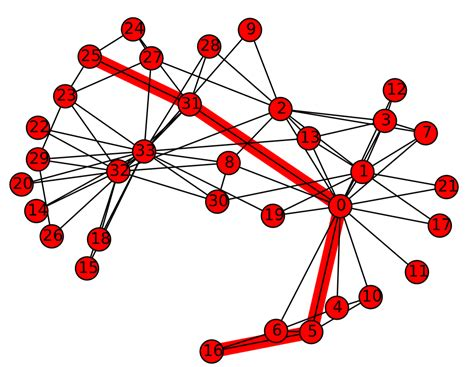
\includegraphics{images/shortest-path.jpeg}

To compute the ASPL of the karate network:

\begin{Shaded}
\begin{Highlighting}[]
\FunctionTok{mean\_distance}\NormalTok{(}\AttributeTok{graph =}\NormalTok{ karate\_uu)}
\end{Highlighting}
\end{Shaded}

\begin{verbatim}
## [1] 2.4082
\end{verbatim}

On average, it takes 2.4 steps to connect any two randomly selected nodes in the karate network.

It is possible to compute ASPL based on shortest paths that consider the direction and weights of the edges.

\begin{Shaded}
\begin{Highlighting}[]
\FunctionTok{mean\_distance}\NormalTok{(karate\_uu, }\AttributeTok{weights =} \ConstantTok{NA}\NormalTok{, }\AttributeTok{directed =}\NormalTok{ F) }\CommentTok{\# unweighted, undirected}
\end{Highlighting}
\end{Shaded}

\begin{verbatim}
## [1] 2.4082
\end{verbatim}

\begin{Shaded}
\begin{Highlighting}[]
\FunctionTok{mean\_distance}\NormalTok{(karate\_uu, }\AttributeTok{weights =} \ConstantTok{NA}\NormalTok{, }\AttributeTok{directed =}\NormalTok{ T) }\CommentTok{\# unweighted, directed }
\end{Highlighting}
\end{Shaded}

\begin{verbatim}
## [1] 2.4082
\end{verbatim}

\begin{Shaded}
\begin{Highlighting}[]
\FunctionTok{mean\_distance}\NormalTok{(karate\_uu, }\AttributeTok{directed =}\NormalTok{ F) }\CommentTok{\# weighted, undirected}
\end{Highlighting}
\end{Shaded}

\begin{verbatim}
## [1] 2.4082
\end{verbatim}

\begin{Shaded}
\begin{Highlighting}[]
\FunctionTok{mean\_distance}\NormalTok{(karate\_uu, }\AttributeTok{directed =}\NormalTok{ T) }\CommentTok{\# weighted, directed }
\end{Highlighting}
\end{Shaded}

\begin{verbatim}
## [1] 2.4082
\end{verbatim}

Because \texttt{karate\_uu} is undirected and unweighted, the result is unsurprisingly identical across all 4 version (try this with a directed, weighted network!). When a graph contains edge weights, then they are automatically considered unless you instruct otherwise using \texttt{weights\ =\ NA}. Use the \texttt{directed} argument to specify if the direction of the edges should be considered in the computation of short paths.

An important point to note is that edge weights are interpreted as \emph{distances} rather than \emph{strength of connection}: See Chapter 7 for more information about this.

\section{Global Clustering Coefficient}\label{global-clustering-coefficient}

\textbf{Global clustering coefficient}, or global \emph{C}, refers to the number of closed triangles in the network relative to the number of possible triangles. It is a measure of overall level of local connectivity among nodes in the network.

A simple way of thinking about this concept is that it is measuring the probability that each pair of ``friends'' of a given node are also friends with each other.

To computer global clustering coefficient, we use the \texttt{transitivity} function as follows:

\begin{Shaded}
\begin{Highlighting}[]
\FunctionTok{transitivity}\NormalTok{(karate\_uu, }\AttributeTok{type =} \StringTok{\textquotesingle{}global\textquotesingle{}}\NormalTok{)}
\end{Highlighting}
\end{Shaded}

\begin{verbatim}
## [1] 0.2556818
\end{verbatim}

We can interpret this value to mean that for each pair of nodes that are directly connected to a target node, the probability that these two nodes are also connected to each other is 25.6\% (i.e., the probability of a completed ``triangle'', when it is possible, is 25.6\%). This value is usually quite high in social networks, because people tend to introduce their friends to each other, resulting in \emph{triadic closure}.

Contrast this with Chapter 7: Local clustering coefficient--notice that although we use the same function, the \texttt{type} argument specifies if we want to obtain the global clustering coefficient for the whole network (overall local connectivity), or local clustering coefficient for individual nodes (local connectivity centered on a single node).

\section{Small World Index}\label{small-world-index}

The term ``small world'' has a specific meaning in network science as compared to the layperson's. A network is considered to have small world characteristics if (i) its ASPL is shorter than that of a randomly generated network with the same number of nodes and edges, and (ii) its global \emph{C} is larger than that of a randomly generated network with the same number of nodes and edges. There are various ways to compute a value that quantifies the ``small worldness'' of a network, although we do not cover all of them here (see Neal, 2017, for a comparison of different methods). In this section we go through an approach to quantifying small-worldness based on Humphries and Gurney (2008).

In practice, researchers compute a measure known as the \textbf{small world index} which combines the global clustering coefficient and ASPL of the target network relative to its equally sized random graphs (with the same number of nodes and edges) to derive a proportional score.

Mathematically,
\[SWI = \frac{C_i / \overline C_{rand}}{L_i / \overline L_{rand}}\]
where \emph{C} = global clustering coefficient, \emph{L} = average shortest path length, \emph{i} = network of interest, \emph{rand} = random network, \(\overline x\) denotes mean of the random networks' measures.

In order to compute the Small World Index we need to first generate networks that form a baseline for comparison to the target network (see also Chapter 9: Network Models). Here, we generate 5 size-matched Erdos-Renyi (ER) networks, which is a type of random network model where edges are distributed randomly across a set of nodes. We specify that the number of nodes and edges of the ER network to be identical to the target network (\texttt{karate\_uu}). Then we take the mean ASPL and C of the ER networks, which becomes the \(\overline L_{rand}\) and \(\overline C_{rand}\) in the equation above respectively.

\begin{Shaded}
\begin{Highlighting}[]
\DocumentationTok{\#\# generate ER networks }
\FunctionTok{set.seed}\NormalTok{(}\DecValTok{2}\NormalTok{)}

\NormalTok{er\_graphs }\OtherTok{\textless{}{-}} \FunctionTok{list}\NormalTok{()}

\ControlFlowTok{for}\NormalTok{(i }\ControlFlowTok{in} \DecValTok{1}\SpecialCharTok{:}\DecValTok{5}\NormalTok{) \{ }\CommentTok{\# number of networks to generate}
\NormalTok{  er\_graphs[[i]] }\OtherTok{\textless{}{-}} \FunctionTok{sample\_gnm}\NormalTok{(}\AttributeTok{n =} \FunctionTok{gorder}\NormalTok{(karate\_uu), }\AttributeTok{m =} \FunctionTok{gsize}\NormalTok{(karate\_uu), }\AttributeTok{directed =}\NormalTok{ F, }\AttributeTok{loops =}\NormalTok{ F)}
\NormalTok{\}}

\CommentTok{\# compute the L and C for each ER network, take the mean }
\FunctionTok{sapply}\NormalTok{(er\_graphs, mean\_distance) }\SpecialCharTok{|\textgreater{}} \FunctionTok{mean}\NormalTok{() }\CommentTok{\# L\_rand}
\end{Highlighting}
\end{Shaded}

\begin{verbatim}
## [1] 2.384314
\end{verbatim}

\begin{Shaded}
\begin{Highlighting}[]
\FunctionTok{sapply}\NormalTok{(er\_graphs, transitivity, }\AttributeTok{type =} \StringTok{\textquotesingle{}global\textquotesingle{}}\NormalTok{) }\SpecialCharTok{|\textgreater{}} \FunctionTok{mean}\NormalTok{() }\CommentTok{\# C\_rand}
\end{Highlighting}
\end{Shaded}

\begin{verbatim}
## [1] 0.1188022
\end{verbatim}

We can now plug in these values together with the actual C and L of the target network to compute SWI:

\begin{Shaded}
\begin{Highlighting}[]
\CommentTok{\# SWI for karate\_uu }
\NormalTok{(}\FloatTok{0.2556818}\SpecialCharTok{/}\FloatTok{0.1188022}\NormalTok{)}\SpecialCharTok{/}\NormalTok{(}\FloatTok{2.4082}\SpecialCharTok{/}\FloatTok{2.384314}\NormalTok{)}
\end{Highlighting}
\end{Shaded}

\begin{verbatim}
## [1] 2.130817
\end{verbatim}

Humphries and Gurney (2008) write that SWI larger than 1 indicates presence of a small world structure, since this implies that the target network has more local clustering than random expectation, while having relatively similar ASPLs. SWIs less than 1 or close to 1 indicates that there is no evidence to support the claim that the target network is a small world. Here, we have some evidence supporting the claim that our karate network has a small world structure. In practice, up to 1,000 random ER networks are generated to compute \(\overline L_{rand}\) and \(\overline C_{rand}\); although this can be a slow process depending on your network size. The number of random networks to generate can be adjusted in the for loop above.

The main take home message is that a small world network has high levels of local clustering (nodes whose neighbors are also neighbors of each other), but also contains a number of shortcuts that drastically reduces the overall distances/path lengths between nodes. See below for an illustration of this idea.

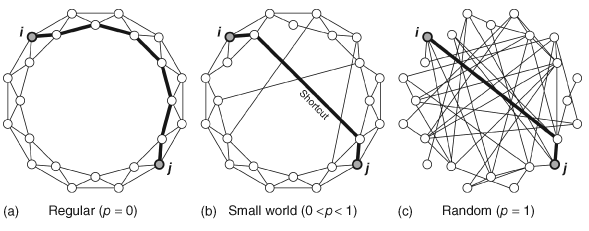
\includegraphics{images/small-world.png}

\section{Network Density}\label{network-density}

\textbf{Network density} refers to the ratio of the number of (existing) edges and the number of possible edges among nodes in the network.

Simple example of networks with lower and higher network densities.

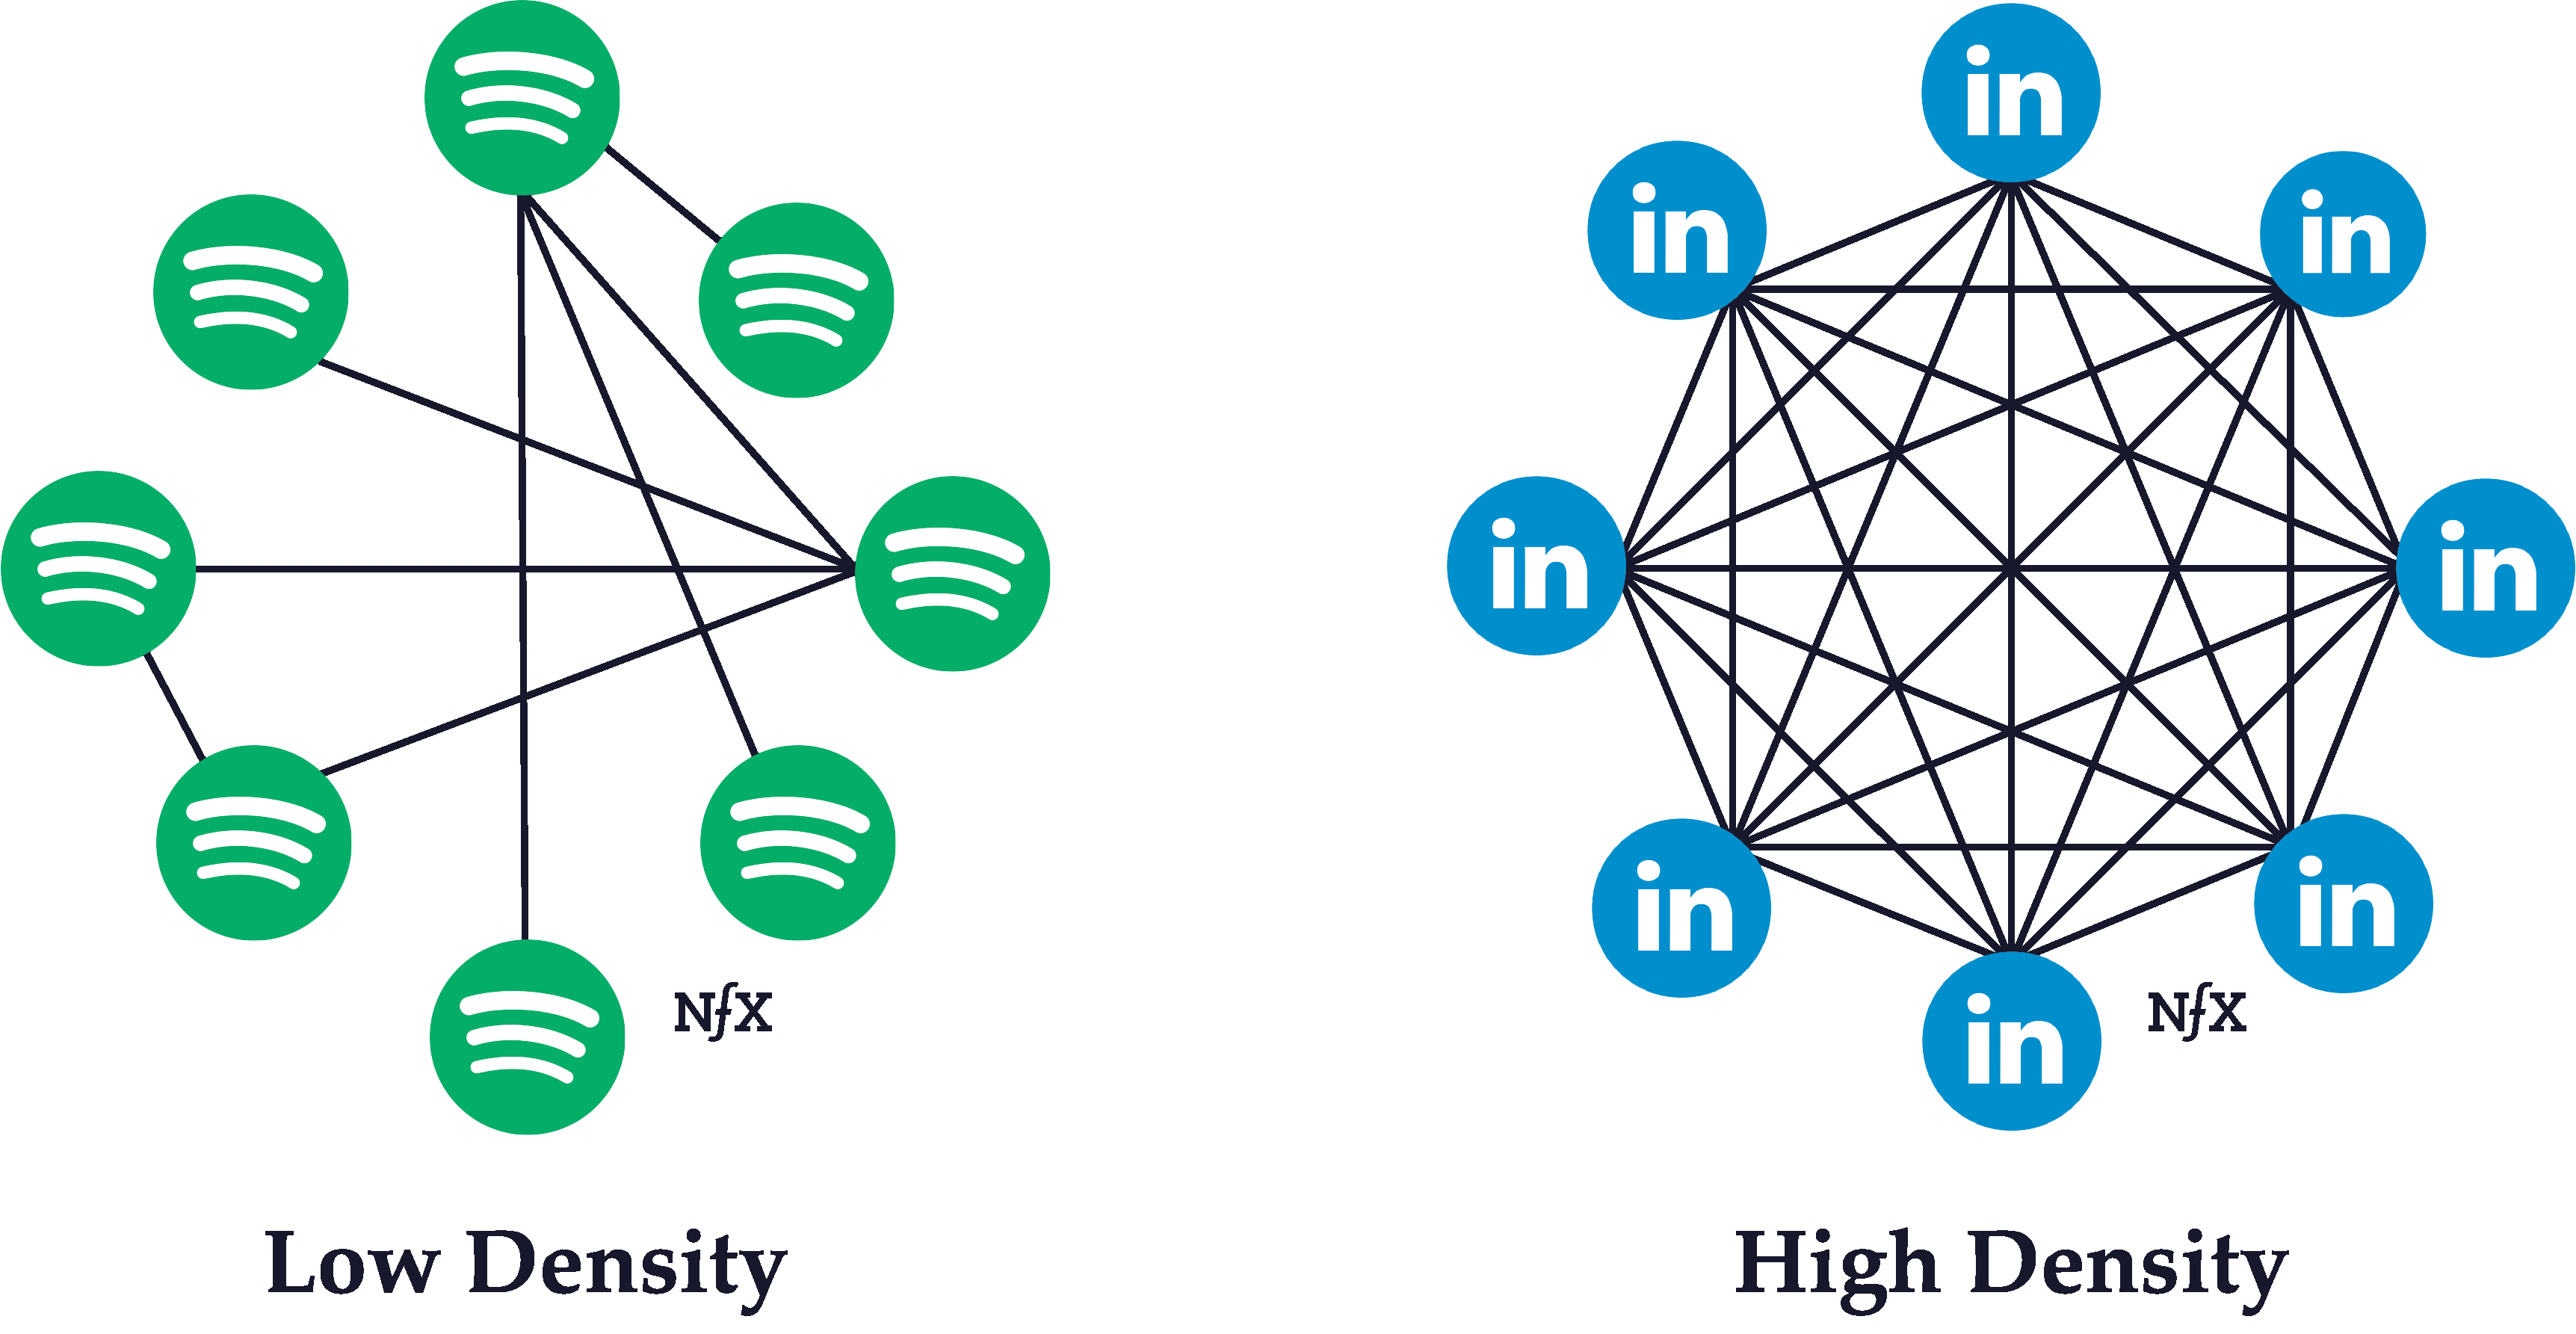
\includegraphics{images/density.png}

To obtain network density of a network:

\begin{Shaded}
\begin{Highlighting}[]
\FunctionTok{edge\_density}\NormalTok{(karate\_uu)}
\end{Highlighting}
\end{Shaded}

\begin{verbatim}
## [1] 0.1390374
\end{verbatim}

This means that 13.9\% of all possible edges in the network are actual edges.

\section{Network Diameter}\label{network-diameter}

Network diameter refers to length of the longest shortest path between nodes in the network. Instead of getting the mean of all the shortest paths as you did in ASPL, what is the maximum length of those short paths?

Simple example of networks with higher and lower network diameters

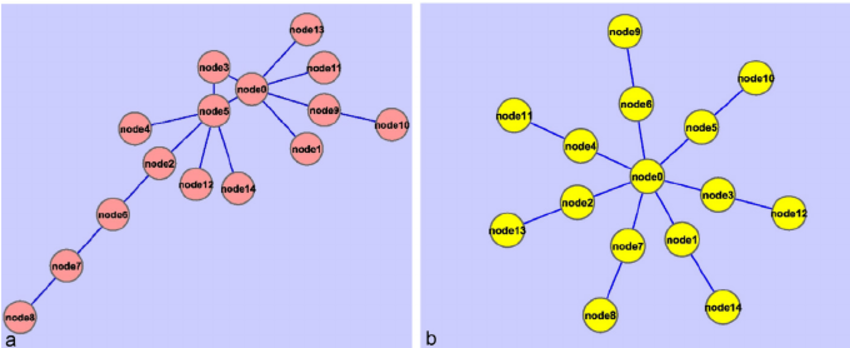
\includegraphics{images/diameter.png}

To obtain network diameter of a network:

\begin{Shaded}
\begin{Highlighting}[]
\FunctionTok{diameter}\NormalTok{(karate\_uu, }\AttributeTok{directed =}\NormalTok{ F)}
\end{Highlighting}
\end{Shaded}

\begin{verbatim}
## [1] 5
\end{verbatim}

\begin{Shaded}
\begin{Highlighting}[]
\CommentTok{\# diameter(karate\_uu, directed = T) \# directed edges }
\end{Highlighting}
\end{Shaded}

This means that the length of the longest shortest path between two nodes in the network is 5.

\section{Assortative Mixing}\label{assortative-mixing}

\textbf{Assortative mixing} is a measure of \emph{homophily} in the network, based on some internal/external property of the nodes. Are nodes that are connected to each other tend to have similar properties?

\subsection{Assortative Mixing by Degree (continuous attributes)}\label{assortative-mixing-by-degree-continuous-attributes}

A common extension of assortative mixing is \textbf{assortative mixing by degree}, which measures the correlation of degrees between neighboring nodes. Are nodes that are connected to each other tend to have similar degrees?

A positive value indicates that nodes that are many (few) neighbors tend to be connected to nodes that also have many (few) neighbors. A negative value indicates that nodes that are many (few) neighbors tend to be connected to nodes that have few (many) neighbors. Values very close to zero indicates no correlation.

\begin{Shaded}
\begin{Highlighting}[]
\FunctionTok{assortativity\_degree}\NormalTok{(karate\_uu, }\AttributeTok{directed =}\NormalTok{ F)}
\end{Highlighting}
\end{Shaded}

\begin{verbatim}
## [1] -0.4756131
\end{verbatim}

\begin{Shaded}
\begin{Highlighting}[]
\CommentTok{\# assortativity\_degree(karate\_uu, directed = T) \# for directed edges }
\end{Highlighting}
\end{Shaded}

There is \emph{dissortativity mixing by degree} in the karate network--nodes with higher degree have a higher tendency to be connected to nodes with lower degree.

It is possible to add your own node attributes to the network (see Chapter 5) and compute its assortativity. The script below demonstrates this with a randomly created set of numbers for the nodes (i.e., a continuous variable ranging from 1 to 5, randomly selected with replacement for each of the 34 nodes in the network). Because these numbers are randomly generated, we expect assortativity to be close to 0 here.

\begin{Shaded}
\begin{Highlighting}[]
\CommentTok{\# create a random vector of numbers for demonstration}
\FunctionTok{set.seed}\NormalTok{(}\DecValTok{3}\NormalTok{)}
\FunctionTok{V}\NormalTok{(karate\_uu)}\SpecialCharTok{$}\NormalTok{random1 }\OtherTok{\textless{}{-}} \FunctionTok{sample}\NormalTok{(}\DecValTok{1}\SpecialCharTok{:}\DecValTok{5}\NormalTok{, }\FunctionTok{gorder}\NormalTok{(karate\_uu), }\AttributeTok{replace =}\NormalTok{ T)}

\CommentTok{\# compute the assortativity of this node attribute }
\FunctionTok{assortativity}\NormalTok{(karate\_uu, }\AttributeTok{values =} \FunctionTok{V}\NormalTok{(karate\_uu)}\SpecialCharTok{$}\NormalTok{random1, }\AttributeTok{directed =}\NormalTok{ F)}
\end{Highlighting}
\end{Shaded}

\begin{verbatim}
## [1] -0.06819853
\end{verbatim}

\subsection{Assortative Mixing by Node Attributes (categorical attributes)}\label{assortative-mixing-by-node-attributes-categorical-attributes}

It is also possible to compute assortativity for categorical labels assigned to nodes. For instance, in a social network of male and female actors, is there gender homophily such that nodes tend to be connected to other nodes that share the same label?

A positive value indicates that nodes with the same labels tend to be connected to each other. A negative value indicates that nodes tend to be connected to nodes with a different label from itself. Values very close to zero indicates no correlation.

It is possible to add your own node attributes to the network (see Chapter 5) and compute its assortativity. The script below demonstrates this with a randomly created set of labels for the nodes (i.e., a categorical variable). Because these labels are randomly generated, we expect assortativity to be close to 0 here.

\begin{Shaded}
\begin{Highlighting}[]
\CommentTok{\# create a random vector of labels for demonstration}
\FunctionTok{set.seed}\NormalTok{(}\DecValTok{3}\NormalTok{)}
\FunctionTok{V}\NormalTok{(karate\_uu)}\SpecialCharTok{$}\NormalTok{random2 }\OtherTok{\textless{}{-}} \FunctionTok{sample}\NormalTok{(}\FunctionTok{c}\NormalTok{(}\StringTok{\textquotesingle{}A\textquotesingle{}}\NormalTok{, }\StringTok{\textquotesingle{}B\textquotesingle{}}\NormalTok{, }\StringTok{\textquotesingle{}C\textquotesingle{}}\NormalTok{), }\FunctionTok{gorder}\NormalTok{(karate\_uu), }\AttributeTok{replace =}\NormalTok{ T)}

\CommentTok{\# compute the assortativity of this node attribute }
\FunctionTok{assortativity\_nominal}\NormalTok{(karate\_uu, }\AttributeTok{types =} \FunctionTok{factor}\NormalTok{(}\FunctionTok{V}\NormalTok{(karate\_uu)}\SpecialCharTok{$}\NormalTok{random2), }\AttributeTok{directed =}\NormalTok{ F)}
\end{Highlighting}
\end{Shaded}

\begin{verbatim}
## [1] -0.0850826
\end{verbatim}

\section{Network Components}\label{network-components}

Thus far, we have been assuming that the networks that we have worked with form a single component. In other words, all nodes are part of the same component, and there are no separate components. But, as shown in the example network below, it is certainly possible for nodes in a network to fragment into distinct components.

\begin{Shaded}
\begin{Highlighting}[]
\CommentTok{\# create a sample network with two distinct components }
\NormalTok{g }\OtherTok{\textless{}{-}} \FunctionTok{graph\_from\_literal}\NormalTok{(A}\SpecialCharTok{{-}}\NormalTok{B, B}\SpecialCharTok{{-}}\NormalTok{C, A}\SpecialCharTok{{-}}\NormalTok{C, D}\SpecialCharTok{{-}}\NormalTok{E)}
\FunctionTok{plot}\NormalTok{(g)}
\end{Highlighting}
\end{Shaded}

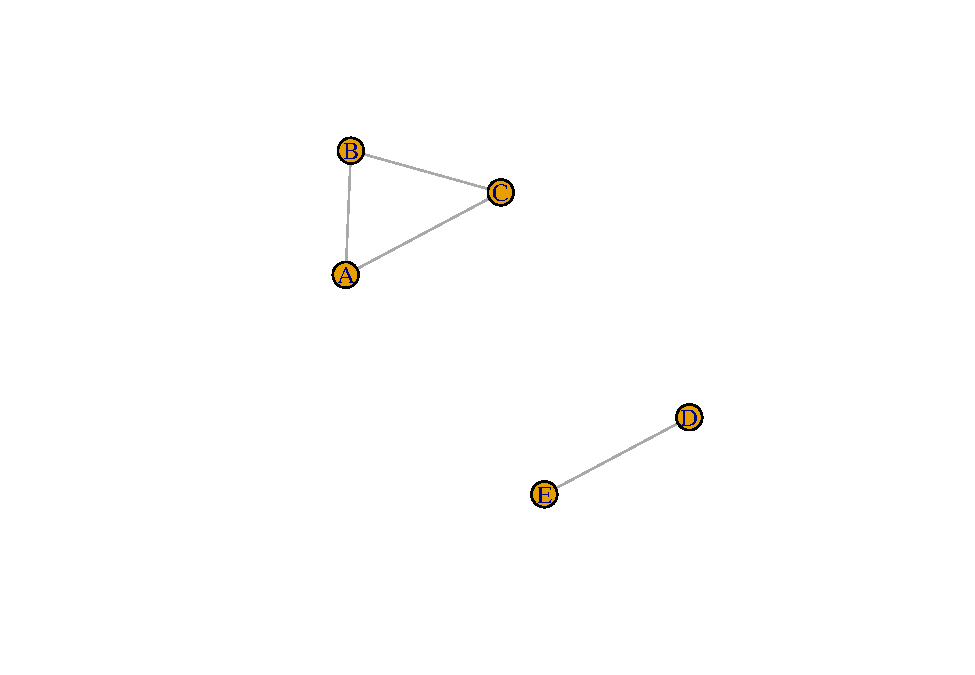
\includegraphics{bookdown-demo_files/figure-latex/unnamed-chunk-110-1.pdf}

When working with networks derived from behavioral data, it can be common to observe that the network consists of distinct network components. This has implications for the computing and interpretation of the macro-level network measures, because several of them rely on the computation of shortest path between node pairs. For instance, ASPL computes the shortest paths for all possible node pairs and takes the mean--but what happens if there is no path between nodes A and D, for example?

Node pairs that do not have a path are ignored in the computation. This is the default behavior in \texttt{igraph}. Hence, this value reflects the mean of all ``computable'' short paths (i.e., when node pairs are found in the same component) and this is computed across all network components in the network.

\begin{Shaded}
\begin{Highlighting}[]
\FunctionTok{mean\_distance}\NormalTok{(g, }\AttributeTok{unconnected =} \ConstantTok{TRUE}\NormalTok{) }\CommentTok{\# ignore infinite paths, default }
\end{Highlighting}
\end{Shaded}

\begin{verbatim}
## [1] 1
\end{verbatim}

\begin{Shaded}
\begin{Highlighting}[]
\FunctionTok{mean\_distance}\NormalTok{(g, }\AttributeTok{unconnected =} \ConstantTok{FALSE}\NormalTok{) }\CommentTok{\# consider infinite paths }
\end{Highlighting}
\end{Shaded}

\begin{verbatim}
## [1] Inf
\end{verbatim}

As you can see, the second output is \texttt{Inf}, reflecting the presence of infinite paths in the network. From the \texttt{igraph} documentation: ``If TRUE, only the lengths of the existing paths are considered and averaged; if FALSE, the length of the missing paths are considered as having infinite length, making the mean distance infinite as well.''

Hence, it is good practice to first check if your network consists of a single component, or multiple components. We can use the following script to find out: how many components, the size of each components (number of nodes), and obtain a list of nodes and their component membership. Basically, \texttt{components} is a special function that stores these pieces of information as its output, which you can then retrieve using the \texttt{\$}: \texttt{csize} for size of component, \texttt{no} for number of components, \texttt{membership} for the component membership for each node.

\begin{Shaded}
\begin{Highlighting}[]
\NormalTok{g\_comp }\OtherTok{\textless{}{-}} \FunctionTok{components}\NormalTok{(g)}

\NormalTok{g\_comp}\SpecialCharTok{$}\NormalTok{csize }\CommentTok{\# size of each component }
\end{Highlighting}
\end{Shaded}

\begin{verbatim}
## [1] 3 2
\end{verbatim}

\begin{Shaded}
\begin{Highlighting}[]
\NormalTok{g\_comp}\SpecialCharTok{$}\NormalTok{no }\CommentTok{\# number of components }
\end{Highlighting}
\end{Shaded}

\begin{verbatim}
## [1] 2
\end{verbatim}

\begin{Shaded}
\begin{Highlighting}[]
\FunctionTok{data.frame}\NormalTok{(}\AttributeTok{node =} \FunctionTok{V}\NormalTok{(g)}\SpecialCharTok{$}\NormalTok{name, }\AttributeTok{membership =}\NormalTok{ g\_comp}\SpecialCharTok{$}\NormalTok{membership)}
\end{Highlighting}
\end{Shaded}

\begin{verbatim}
##   node membership
## A    A          1
## B    B          1
## C    C          1
## D    D          2
## E    E          2
\end{verbatim}

\begin{Shaded}
\begin{Highlighting}[]
\CommentTok{\# you should know how to export the results into a .csv file! }
\end{Highlighting}
\end{Shaded}

Typically, real-world networks have a giant or largest connected component (LCC) which contains the majority of nodes in the network, and researchers prefer to only compute network-level metrics on the LCC. This component is extracted for further analysis, removing the smaller connected components or hermits (isolates in the network where the node has no neighbors).

The code below shows you how to extract the largest connected component of the sample network:

\begin{Shaded}
\begin{Highlighting}[]
\NormalTok{g\_lcc }\OtherTok{\textless{}{-}} \FunctionTok{induced\_subgraph}\NormalTok{(}\AttributeTok{graph =}\NormalTok{ g, }
                          \AttributeTok{vids =} \FunctionTok{components}\NormalTok{(g)}\SpecialCharTok{$}\NormalTok{membership }\SpecialCharTok{==} \FunctionTok{which.max}\NormalTok{(}\FunctionTok{components}\NormalTok{(g)}\SpecialCharTok{$}\NormalTok{csize)) }

\FunctionTok{summary}\NormalTok{(g\_lcc)}
\end{Highlighting}
\end{Shaded}

\begin{verbatim}
## IGRAPH 3487066 UN-- 3 3 -- 
## + attr: name (v/c)
\end{verbatim}

It is also possible to extract other components of the network. The code below retains nodes that do not belong to the largest connected component of the network.

\begin{Shaded}
\begin{Highlighting}[]
\NormalTok{g\_2 }\OtherTok{\textless{}{-}} \FunctionTok{induced\_subgraph}\NormalTok{(}\AttributeTok{graph =}\NormalTok{ g, }
                          \AttributeTok{vids =} \FunctionTok{components}\NormalTok{(g)}\SpecialCharTok{$}\NormalTok{membership }\SpecialCharTok{!=} \FunctionTok{which.max}\NormalTok{(}\FunctionTok{components}\NormalTok{(g)}\SpecialCharTok{$}\NormalTok{csize)) }

\FunctionTok{summary}\NormalTok{(g\_2)}
\end{Highlighting}
\end{Shaded}

\begin{verbatim}
## IGRAPH e23b4aa UN-- 2 1 -- 
## + attr: name (v/c)
\end{verbatim}

\section{Exercise}\label{exercise-4}

Your task is to:

\begin{enumerate}
\def\labelenumi{\arabic{enumi}.}
\tightlist
\item
  Load the \texttt{UKfaculty} network from the \texttt{igraphdata} library using the following code:
\end{enumerate}

\begin{Shaded}
\begin{Highlighting}[]
\FunctionTok{library}\NormalTok{(igraphdata) }\CommentTok{\# have you downloaded the package? }

\FunctionTok{data}\NormalTok{(}\StringTok{"UKfaculty"}\NormalTok{) }\CommentTok{\# you should see a UKfaculty object appear in your Environment}

\CommentTok{\# I\textquotesingle{}ve included this code to make it an undirected, unweighted network for this exercise}
\CommentTok{\# for more information about network manipulation, see Chapter 5}
\NormalTok{UKfaculty }\OtherTok{\textless{}{-}}\NormalTok{ UKfaculty }\SpecialCharTok{|\textgreater{}} \FunctionTok{delete\_edge\_attr}\NormalTok{(}\StringTok{"weight"}\NormalTok{) }\SpecialCharTok{|\textgreater{}} \FunctionTok{as.undirected}\NormalTok{(}\AttributeTok{mode =} \StringTok{\textquotesingle{}mutual\textquotesingle{}}\NormalTok{)}
\end{Highlighting}
\end{Shaded}

\{TODO: Briefly describe the network.\}

\begin{enumerate}
\def\labelenumi{\arabic{enumi}.}
\setcounter{enumi}{1}
\tightlist
\item
  Answer the following questions:
\end{enumerate}

\begin{itemize}
\item
  How many nodes and edges does the network have?
\item
  How many network components does this network have? If it has more than one component, only retain the largest connected component before proceeding to the next part.
\item
  Compute the following macro-level network measures for this network:

  \begin{itemize}
  \tightlist
  \item
    average degree
  \item
    average shortest path length
  \item
    global clustering coefficient
  \item
    network density
  \item
    network diameter
  \item
    assortativity (by degree and by group) \{footnote\}
  \item
    small world index
  \end{itemize}
\end{itemize}

Footnote: \texttt{UKfaculty} contains a \texttt{Group} node attribute which denotes the department that each faculty member belonged to.

\chapter{Chapter 7: Micro-level network measures}\label{ch7}

Micro-level network measures provide you with information about specific nodes in the network. These are generally known as centrality measures in the network science literature. Centrality is the network scientist's way of quantifying the relative ``importance'' of a given node relative to other nodes in the network. There are \emph{many} different definitions of what counts as ``central'', as you will see in the following subsections, and also from this \href{http://schochastics.net/sna/periodic.html}{Periodic Table of Centrality Indices}. There is no single ``correct'' or ``best'' metric - which metrics are most useful to you will depend on the nature of the system that you are modeling as well as the network behavior that you interested in.

To facilitate the demonstrations below, we will use the directed, weighted karate network that we have previously seen in Chapter 4. In the rest of the chapter we will compute various micro-level network measures for the nodes in this network.

\begin{Shaded}
\begin{Highlighting}[]
\NormalTok{karate\_el }\OtherTok{\textless{}{-}} \FunctionTok{read.csv}\NormalTok{(}\StringTok{\textquotesingle{}data/karate\_el\_weights.csv\textquotesingle{}}\NormalTok{, }\AttributeTok{header =} \ConstantTok{TRUE}\NormalTok{)}

\NormalTok{karate\_dw }\OtherTok{\textless{}{-}} \FunctionTok{graph\_from\_data\_frame}\NormalTok{(karate\_el, }\AttributeTok{directed =} \ConstantTok{TRUE}\NormalTok{)}

\FunctionTok{summary}\NormalTok{(karate\_dw)}
\end{Highlighting}
\end{Shaded}

\begin{verbatim}
## IGRAPH 66f644c DNW- 34 78 -- 
## + attr: name (v/c), weight (e/n)
\end{verbatim}

\section{Degree}\label{degree}

The \textbf{degree} of node \emph{i}, frequently denoted as \emph{k\_i} in the network science literature, refers to the number of edges or links directly connected to node \emph{i}.

To get the degree of all nodes in the network, try running the following code:

\begin{Shaded}
\begin{Highlighting}[]
\FunctionTok{degree}\NormalTok{(}\AttributeTok{graph =}\NormalTok{ karate\_dw)}
\end{Highlighting}
\end{Shaded}

\begin{verbatim}
##    Mr Hi  Actor 2  Actor 3  Actor 4  Actor 5  Actor 6  Actor 7  Actor 9 Actor 10 Actor 14 Actor 15 Actor 16 Actor 19 Actor 20 Actor 21 Actor 23 Actor 24 Actor 25 Actor 26 Actor 27 Actor 28 Actor 29 Actor 30 Actor 31 
##       16        9       10        6        3        4        4        5        2        5        2        2        2        3        2        2        5        3        3        2        4        3        4        4 
## Actor 32 Actor 33  Actor 8 Actor 11 Actor 12 Actor 13 Actor 18 Actor 22 Actor 17   John A 
##        6       12        4        3        1        2        2        2        2       17
\end{verbatim}

If you only want the degree for a specific node:

\begin{Shaded}
\begin{Highlighting}[]
\FunctionTok{degree}\NormalTok{(}\AttributeTok{graph =}\NormalTok{ karate\_dw, }\AttributeTok{v =} \StringTok{\textquotesingle{}Mr Hi\textquotesingle{}}\NormalTok{)}
\end{Highlighting}
\end{Shaded}

\begin{verbatim}
## Mr Hi 
##    16
\end{verbatim}

\begin{Shaded}
\begin{Highlighting}[]
\FunctionTok{degree}\NormalTok{(}\AttributeTok{graph =}\NormalTok{ karate\_dw, }\AttributeTok{v =} \FunctionTok{c}\NormalTok{(}\StringTok{\textquotesingle{}Mr Hi\textquotesingle{}}\NormalTok{, }\StringTok{\textquotesingle{}Actor 5\textquotesingle{}}\NormalTok{)) }\CommentTok{\# for more than 1 node}
\end{Highlighting}
\end{Shaded}

\begin{verbatim}
##   Mr Hi Actor 5 
##      16       3
\end{verbatim}

It would be better to ``save'' the outputs as an object (especially if your network is very large!) so that you can manipulate or export it later.

\begin{Shaded}
\begin{Highlighting}[]
\NormalTok{karate\_degree }\OtherTok{\textless{}{-}} \FunctionTok{degree}\NormalTok{(karate\_dw)}
\end{Highlighting}
\end{Shaded}

Notice that you have a named vector called \texttt{karate\_degree} in your Environment.

\subsection{In-, out-, all-degree}\label{in--out--all-degree}

If your network has directed edges, \textbf{in-degree} refers to the number of edges that are going towards the target node, whereas \textbf{out-degree} refers to the number of edges that are going away from the target node. \textbf{all-degree} is the sum of in-degree and out-degree, and is the same as \emph{degree}.

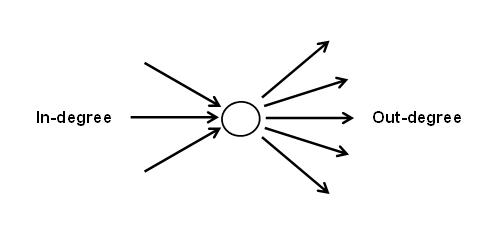
\includegraphics{images/in_out_degree.jpg}

To get the in- or out-degree of a node, we need to include the \texttt{mode\ =\ \textquotesingle{}in\textquotesingle{}} or \texttt{mode\ =\ \textquotesingle{}out\textquotesingle{}} argument accordingly.

\begin{Shaded}
\begin{Highlighting}[]
\FunctionTok{degree}\NormalTok{(}\AttributeTok{graph =}\NormalTok{ karate\_dw, }\AttributeTok{v =} \StringTok{\textquotesingle{}Actor 5\textquotesingle{}}\NormalTok{, }\AttributeTok{mode =} \StringTok{\textquotesingle{}in\textquotesingle{}}\NormalTok{) }\CommentTok{\# in{-}degree = incoming edges}
\end{Highlighting}
\end{Shaded}

\begin{verbatim}
## Actor 5 
##       1
\end{verbatim}

\begin{Shaded}
\begin{Highlighting}[]
\FunctionTok{degree}\NormalTok{(}\AttributeTok{graph =}\NormalTok{ karate\_dw, }\AttributeTok{v =} \StringTok{\textquotesingle{}Actor 5\textquotesingle{}}\NormalTok{, }\AttributeTok{mode =} \StringTok{\textquotesingle{}out\textquotesingle{}}\NormalTok{) }\CommentTok{\# out{-}degree = outgoing edges}
\end{Highlighting}
\end{Shaded}

\begin{verbatim}
## Actor 5 
##       2
\end{verbatim}

Notice that Actor 5 has an in-degree of 1 and out-degree of 2, and in the previous section we saw that Actor 5 had a degree of 3. If no arguments are specified, \texttt{igraph} will compute all-degree, which is the sum of a node's in- and out-degree, by default for directed graphs. Keep this in mind!

\begin{Shaded}
\begin{Highlighting}[]
\FunctionTok{degree}\NormalTok{(}\AttributeTok{graph =}\NormalTok{ karate\_dw, }\AttributeTok{v =} \StringTok{\textquotesingle{}Actor 5\textquotesingle{}}\NormalTok{) }\CommentTok{\# the default is all{-}degree}
\end{Highlighting}
\end{Shaded}

\begin{verbatim}
## Actor 5 
##       3
\end{verbatim}

\begin{Shaded}
\begin{Highlighting}[]
\FunctionTok{degree}\NormalTok{(}\AttributeTok{graph =}\NormalTok{ karate\_dw, }\AttributeTok{v =} \StringTok{\textquotesingle{}Actor 5\textquotesingle{}}\NormalTok{, }\AttributeTok{mode =} \StringTok{\textquotesingle{}all\textquotesingle{}}\NormalTok{) }
\end{Highlighting}
\end{Shaded}

\begin{verbatim}
## Actor 5 
##       3
\end{verbatim}

\begin{Shaded}
\begin{Highlighting}[]
\FunctionTok{degree}\NormalTok{(}\AttributeTok{graph =}\NormalTok{ karate\_dw, }\AttributeTok{v =} \StringTok{\textquotesingle{}Actor 5\textquotesingle{}}\NormalTok{, }\AttributeTok{mode =} \StringTok{\textquotesingle{}total\textquotesingle{}}\NormalTok{) }\CommentTok{\# all is the same as total}
\end{Highlighting}
\end{Shaded}

\begin{verbatim}
## Actor 5 
##       3
\end{verbatim}

\section{Strength}\label{strength}

The \textbf{strength} of node \emph{i} refers to the sum of its adjacent edge weights. This measure is only applicable to weighted networks.

To get the strength of all nodes in the network, try running the following code:

\begin{Shaded}
\begin{Highlighting}[]
\FunctionTok{strength}\NormalTok{(}\AttributeTok{graph =}\NormalTok{ karate\_dw)}
\end{Highlighting}
\end{Shaded}

\begin{verbatim}
##    Mr Hi  Actor 2  Actor 3  Actor 4  Actor 5  Actor 6  Actor 7  Actor 9 Actor 10 Actor 14 Actor 15 Actor 16 Actor 19 Actor 20 Actor 21 Actor 23 Actor 24 Actor 25 Actor 26 Actor 27 Actor 28 Actor 29 Actor 30 Actor 31 
##       45       23       33       16        4       12       11       16        5       17        6        7        5        9        2        9       22       11        7        4       13        9       12       11 
## Actor 32 Actor 33  Actor 8 Actor 11 Actor 12 Actor 13 Actor 18 Actor 22 Actor 17   John A 
##       17       31        8        5        1        7        7        3        5       53
\end{verbatim}

If you only want the strength for a specific node(s):

\begin{Shaded}
\begin{Highlighting}[]
\FunctionTok{strength}\NormalTok{(}\AttributeTok{graph =}\NormalTok{ karate\_dw, }\AttributeTok{v =} \StringTok{\textquotesingle{}Mr Hi\textquotesingle{}}\NormalTok{)}
\end{Highlighting}
\end{Shaded}

\begin{verbatim}
## Mr Hi 
##    45
\end{verbatim}

\begin{Shaded}
\begin{Highlighting}[]
\FunctionTok{strength}\NormalTok{(}\AttributeTok{graph =}\NormalTok{ karate\_dw, }\AttributeTok{v =} \FunctionTok{c}\NormalTok{(}\StringTok{\textquotesingle{}Mr Hi\textquotesingle{}}\NormalTok{, }\StringTok{\textquotesingle{}Actor 5\textquotesingle{}}\NormalTok{)) }\CommentTok{\# for more than 1 node}
\end{Highlighting}
\end{Shaded}

\begin{verbatim}
##   Mr Hi Actor 5 
##      45       4
\end{verbatim}

\subsection{In-, out-, all-strength}\label{in--out--all-strength}

If your network has directed edges, we can have variations to the original strength measure just as we saw for degree. \textbf{In-strength} refers to the sum of the edge weights that are going towards the target node, whereas \textbf{out-strength} refers to the sum of the edge weights that are going away from the target node. \textbf{all-strength} is the sum of in-strength and out-strength, and is the same as \emph{strength}.

To get the in- or out-strength of a node, we need to include the \texttt{mode\ =\ \textquotesingle{}in\textquotesingle{}} or \texttt{mode\ =\ \textquotesingle{}out\textquotesingle{}} argument accordingly.

\begin{Shaded}
\begin{Highlighting}[]
\FunctionTok{strength}\NormalTok{(}\AttributeTok{graph =}\NormalTok{ karate\_dw, }\AttributeTok{v =} \StringTok{\textquotesingle{}Actor 5\textquotesingle{}}\NormalTok{, }\AttributeTok{mode =} \StringTok{\textquotesingle{}in\textquotesingle{}}\NormalTok{) }\CommentTok{\# in{-}degree = incoming edges}
\end{Highlighting}
\end{Shaded}

\begin{verbatim}
## Actor 5 
##       2
\end{verbatim}

\begin{Shaded}
\begin{Highlighting}[]
\FunctionTok{strength}\NormalTok{(}\AttributeTok{graph =}\NormalTok{ karate\_dw, }\AttributeTok{v =} \StringTok{\textquotesingle{}Actor 5\textquotesingle{}}\NormalTok{, }\AttributeTok{mode =} \StringTok{\textquotesingle{}out\textquotesingle{}}\NormalTok{) }\CommentTok{\# out{-}degree = outgoing edges}
\end{Highlighting}
\end{Shaded}

\begin{verbatim}
## Actor 5 
##       2
\end{verbatim}

It is worth noting here that the in-strength and out-strength of Actor 5 is the same, but recall from the degree section that the in-degree and out-degree of Actor 5 differed. This is a key point to remember, is that strength does \emph{not} provide you with information about the \emph{number} of edges the node has - it is possible for a node to have high strength due to a few highly weighted edges or several weakly weighted edges.

Once again, if no arguments are specified, \texttt{igraph} will compute all-strength, which is the sum of a node's in- and out-strength, by default for directed graphs.

\begin{Shaded}
\begin{Highlighting}[]
\FunctionTok{strength}\NormalTok{(}\AttributeTok{graph =}\NormalTok{ karate\_dw, }\AttributeTok{v =} \StringTok{\textquotesingle{}Actor 5\textquotesingle{}}\NormalTok{) }\CommentTok{\# the default is all{-}strength}
\end{Highlighting}
\end{Shaded}

\begin{verbatim}
## Actor 5 
##       4
\end{verbatim}

\begin{Shaded}
\begin{Highlighting}[]
\FunctionTok{strength}\NormalTok{(}\AttributeTok{graph =}\NormalTok{ karate\_dw, }\AttributeTok{v =} \StringTok{\textquotesingle{}Actor 5\textquotesingle{}}\NormalTok{, }\AttributeTok{mode =} \StringTok{\textquotesingle{}all\textquotesingle{}}\NormalTok{) }
\end{Highlighting}
\end{Shaded}

\begin{verbatim}
## Actor 5 
##       4
\end{verbatim}

\begin{Shaded}
\begin{Highlighting}[]
\FunctionTok{strength}\NormalTok{(}\AttributeTok{graph =}\NormalTok{ karate\_dw, }\AttributeTok{v =} \StringTok{\textquotesingle{}Actor 5\textquotesingle{}}\NormalTok{, }\AttributeTok{mode =} \StringTok{\textquotesingle{}total\textquotesingle{}}\NormalTok{) }\CommentTok{\# all is the same as total}
\end{Highlighting}
\end{Shaded}

\begin{verbatim}
## Actor 5 
##       4
\end{verbatim}

\section{Local clustering coefficient}\label{local-clustering-coefficient}

The \textbf{local clustering coefficient}, \emph{C}, of node \emph{i} measures the ratio of the actual number of edges existing among nodes directly connected to the target node \emph{i} to the number of all possible edges that could exist among these nodes.

\emph{C} ranges from 0 to 1. When \(C = 0\), none of the neighbors of the target node are connected to each other. When \(C = 1\), each neighbor of the target node is connected to all the other neighbors of the target word.

You can think of local clustering coefficient as providing a measure of the \emph{level of interconnectivity among the local neighborhood of the target node}. If you look at the figure below, you can easily see that it is possible for nodes to have the same degree, but different local clustering coefficients.

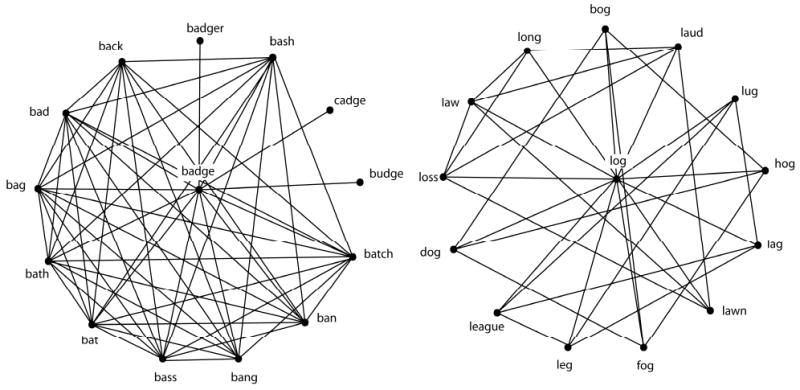
\includegraphics{images/hcc-lcc.jpg}
To get the local clustering coefficient of all nodes in the network, try running the following code:

\begin{Shaded}
\begin{Highlighting}[]
\FunctionTok{transitivity}\NormalTok{(karate\_dw, }\AttributeTok{type =} \StringTok{\textquotesingle{}local\textquotesingle{}}\NormalTok{, }\AttributeTok{isolates =} \StringTok{\textquotesingle{}zero\textquotesingle{}}\NormalTok{)}
\end{Highlighting}
\end{Shaded}

\begin{verbatim}
##     Mr Hi   Actor 2   Actor 3   Actor 4   Actor 5   Actor 6   Actor 7   Actor 9  Actor 10  Actor 14  Actor 15  Actor 16  Actor 19  Actor 20  Actor 21  Actor 23  Actor 24  Actor 25  Actor 26  Actor 27  Actor 28 
## 0.1500000 0.3333333 0.2444444 0.6666667 0.6666667 0.5000000 0.5000000 0.5000000 0.0000000 0.6000000 1.0000000 1.0000000 1.0000000 0.3333333 1.0000000 1.0000000 0.4000000 0.3333333 0.3333333 1.0000000 0.1666667 
##  Actor 29  Actor 30  Actor 31  Actor 32  Actor 33   Actor 8  Actor 11  Actor 12  Actor 13  Actor 18  Actor 22  Actor 17    John A 
## 0.3333333 0.6666667 0.5000000 0.2000000 0.1969697 1.0000000 0.6666667 0.0000000 1.0000000 1.0000000 1.0000000 1.0000000 0.1102941
\end{verbatim}

A couple of things to note:

\begin{enumerate}
\def\labelenumi{\arabic{enumi}.}
\item
  It is important to specify \texttt{type\ =\ local} for local clustering coefficients (one value for each node), as compared to the global clustering coefficient of the entire graph (this is a macro-level measure that we learned about in Chapter 6).
\item
  For nodes that have a degree of 0 or 1, it would not be possible to compute a local clustering coefficient value for those nodes. Be default \texttt{igraph} will return a \texttt{NaN} value (see Actor 12's value below). By specifying \texttt{isolates\ =\ \textquotesingle{}zero\textquotesingle{}} these \texttt{NaN} values will be reported as zeros instead.
\end{enumerate}

\begin{Shaded}
\begin{Highlighting}[]
\FunctionTok{transitivity}\NormalTok{(karate\_dw, }\AttributeTok{type =} \StringTok{\textquotesingle{}local\textquotesingle{}}\NormalTok{)}
\end{Highlighting}
\end{Shaded}

\begin{verbatim}
##     Mr Hi   Actor 2   Actor 3   Actor 4   Actor 5   Actor 6   Actor 7   Actor 9  Actor 10  Actor 14  Actor 15  Actor 16  Actor 19  Actor 20  Actor 21  Actor 23  Actor 24  Actor 25  Actor 26  Actor 27  Actor 28 
## 0.1500000 0.3333333 0.2444444 0.6666667 0.6666667 0.5000000 0.5000000 0.5000000 0.0000000 0.6000000 1.0000000 1.0000000 1.0000000 0.3333333 1.0000000 1.0000000 0.4000000 0.3333333 0.3333333 1.0000000 0.1666667 
##  Actor 29  Actor 30  Actor 31  Actor 32  Actor 33   Actor 8  Actor 11  Actor 12  Actor 13  Actor 18  Actor 22  Actor 17    John A 
## 0.3333333 0.6666667 0.5000000 0.2000000 0.1969697 1.0000000 0.6666667       NaN 1.0000000 1.0000000 1.0000000 1.0000000 0.1102941
\end{verbatim}

\subsection{Weighted local clustering coefficient}\label{weighted-local-clustering-coefficient}

If you have a weighted network, you can compute \emph{weighted} local clustering coefficients using Barrat et al.'s (2004) generalization of transitivity to weighted networks by specifying \texttt{type\ =\ \textquotesingle{}weighted\textquotesingle{}}. If your network is unweighted, this generalization will simply return unweighted C values.

\begin{Shaded}
\begin{Highlighting}[]
\FunctionTok{transitivity}\NormalTok{(karate\_dw, }\AttributeTok{type =} \StringTok{\textquotesingle{}weighted\textquotesingle{}}\NormalTok{)}
\end{Highlighting}
\end{Shaded}

\begin{verbatim}
##      Mr Hi    Actor 2    Actor 3    Actor 4    Actor 5    Actor 6    Actor 7    Actor 9   Actor 10   Actor 14   Actor 15   Actor 16   Actor 19   Actor 20   Actor 21   Actor 23   Actor 24   Actor 25   Actor 26 
## 0.13629630 0.31521739 0.25925926 0.63750000 0.75000000 0.58333333 0.54545455 0.48437500 0.00000000 0.70588235 1.00000000 1.00000000 1.00000000 0.22222222 1.00000000 1.00000000 0.38636364 0.27272727 0.14285714 
##   Actor 27   Actor 28   Actor 29   Actor 30   Actor 31   Actor 32   Actor 33    Actor 8   Actor 11   Actor 12   Actor 13   Actor 18   Actor 22   Actor 17     John A 
## 1.00000000 0.15384615 0.27777778 0.75000000 0.60606061 0.16470588 0.15542522 1.00000000 0.80000000        NaN 1.00000000 1.00000000 1.00000000 1.00000000 0.09669811
\end{verbatim}

\section{Closeness centrality}\label{closeness-centrality}

\textbf{Closeness centrality} of node \emph{i} is the inverse of the average of the length of the shortest path between node \emph{i} and all other nodes in the network. If a node has high closeness centrality, it means that on average, it takes few steps to travel from that node to all other nodes in the network. If a node has low closeness centrality, it means that on average, it takes more steps to travel from that node to all other nodes in the network.

Closeness centrality is commonly viewed as an indicator of the accessibility of a given node in the network from all other locations in the network.

To get the closeness centrality of all nodes in the network, try running the following code:

\begin{Shaded}
\begin{Highlighting}[]
\FunctionTok{closeness}\NormalTok{(karate\_dw, }\AttributeTok{normalized =}\NormalTok{ T) }\CommentTok{\# weights are automatically considered}
\end{Highlighting}
\end{Shaded}

\begin{verbatim}
##     Mr Hi   Actor 2   Actor 3   Actor 4   Actor 5   Actor 6   Actor 7   Actor 9  Actor 10  Actor 14  Actor 15  Actor 16  Actor 19  Actor 20  Actor 21  Actor 23  Actor 24  Actor 25  Actor 26  Actor 27  Actor 28 
## 0.2771084 0.2051282 0.2666667 0.2666667 0.5000000 0.4285714 0.3333333 0.4285714 0.5000000 1.0000000 0.3333333 0.2857143 0.6666667 0.2000000 1.0000000 0.2222222 0.2142857 0.3125000 0.4285714 0.4285714 0.5000000 
##  Actor 29  Actor 30  Actor 31  Actor 32  Actor 33   Actor 8  Actor 11  Actor 12  Actor 13  Actor 18  Actor 22  Actor 17    John A 
## 0.3333333 0.4000000 0.2857143 0.5000000 1.0000000       NaN       NaN       NaN       NaN       NaN       NaN       NaN       NaN
\end{verbatim}

It is typical to include \texttt{normalized\ =\ T} so that the values are normalized with respect to the size of the network.

Note that closeness centrality can only be meaningfully computed for connected graphs (so that a path exists between any pair of nodes; see Chapter 6: Network Components). If there are distinct network components in the network, this means that for some sets of node pairs, the path between them does not exist and closeness cannot be computed. Usually, network scientists focus their analysis on the largest connected component of the network and ignore the smaller connected components (which are typically viewed as outliers). Chapter 6 provides you with the code needed to extract the largest connected component from the initial network.

You can specify the \texttt{mode} and \texttt{weights} arguments accordingly if you have directed/weighted networks to get the corresponding versions of closeness centrality computed.

\subsection{Weighted closeness centrality}\label{weighted-closeness-centrality}

If your network is weighted, weights are automatically included in the computation of closeness centrality. If you prefer that edge weights are \emph{not} considered, include \texttt{weights\ =\ NA} in the argument. Notice that some of the values have changed depending on whether weights are considered or not.

If your network is unweighted, then weights are not considered by default.

\begin{Shaded}
\begin{Highlighting}[]
\FunctionTok{closeness}\NormalTok{(karate\_dw, }\AttributeTok{normalized =}\NormalTok{ T) }\CommentTok{\# weights are automatically considered}
\end{Highlighting}
\end{Shaded}

\begin{verbatim}
##     Mr Hi   Actor 2   Actor 3   Actor 4   Actor 5   Actor 6   Actor 7   Actor 9  Actor 10  Actor 14  Actor 15  Actor 16  Actor 19  Actor 20  Actor 21  Actor 23  Actor 24  Actor 25  Actor 26  Actor 27  Actor 28 
## 0.2771084 0.2051282 0.2666667 0.2666667 0.5000000 0.4285714 0.3333333 0.4285714 0.5000000 1.0000000 0.3333333 0.2857143 0.6666667 0.2000000 1.0000000 0.2222222 0.2142857 0.3125000 0.4285714 0.4285714 0.5000000 
##  Actor 29  Actor 30  Actor 31  Actor 32  Actor 33   Actor 8  Actor 11  Actor 12  Actor 13  Actor 18  Actor 22  Actor 17    John A 
## 0.3333333 0.4000000 0.2857143 0.5000000 1.0000000       NaN       NaN       NaN       NaN       NaN       NaN       NaN       NaN
\end{verbatim}

\begin{Shaded}
\begin{Highlighting}[]
\FunctionTok{closeness}\NormalTok{(karate\_dw, }\AttributeTok{normalized =}\NormalTok{ T, }\AttributeTok{weights =} \ConstantTok{NA}\NormalTok{) }\CommentTok{\# weights are ignored}
\end{Highlighting}
\end{Shaded}

\begin{verbatim}
##     Mr Hi   Actor 2   Actor 3   Actor 4   Actor 5   Actor 6   Actor 7   Actor 9  Actor 10  Actor 14  Actor 15  Actor 16  Actor 19  Actor 20  Actor 21  Actor 23  Actor 24  Actor 25  Actor 26  Actor 27  Actor 28 
## 0.7666667 0.6400000 0.7500000 0.8000000 0.7500000 1.0000000 1.0000000 1.0000000 1.0000000 1.0000000 1.0000000 1.0000000 1.0000000 1.0000000 1.0000000 1.0000000 0.8571429 0.7142857 0.6000000 0.7500000 1.0000000 
##  Actor 29  Actor 30  Actor 31  Actor 32  Actor 33   Actor 8  Actor 11  Actor 12  Actor 13  Actor 18  Actor 22  Actor 17    John A 
## 0.7500000 1.0000000 1.0000000 1.0000000 1.0000000       NaN       NaN       NaN       NaN       NaN       NaN       NaN       NaN
\end{verbatim}

\subsection{Interpretation of edge weights}\label{interpretation-of-edge-weights}

Caution is needed as the interpretation of edge weights in this context is to treat them as \emph{distances} rather than as connection strengths. In other words, when computing closeness centralities, \texttt{igraph} treats higher edge weights as longer distances. As reproduced from the \texttt{igraph} documentation: ``If the graph has a weight edge attribute, then this is used by default. Weights are used for calculating weighted shortest paths, so they are interpreted as distances.'').

Notice that this is different from how we would normally want to interpret edge weights, usually as indicator of the strength of the relation between two nodes. If we want the weights to be interpreted in the way that we intend (as relational strength) we need to include the following to ``trick'' igraph: \texttt{weights\ =\ 1/E(network)\$weight}. This inverts the relation so that now bigger numbers for edge weight corresponds to shorter distances (and hence shorter paths).

To demonstrate this point consider the simple example below where we wish to compute the shortest path between two nodes in unweighted and weighted networks. Notice that the result changes depending on the weights assigned to the edges--whereby smaller weights are considered to provide ``shorter paths'' between pairs of nodes. This corresponds to the ``distance'' interpretation of edge weights. Because closeness centrality relies on the same \texttt{shortest\_paths} function under the hood, this is something that we need to keep in mind when deciding to computed weighted closeness centrality.

\begin{Shaded}
\begin{Highlighting}[]
\CommentTok{\# unweighted graph}
\NormalTok{g }\OtherTok{\textless{}{-}} \FunctionTok{graph\_from\_literal}\NormalTok{(A}\SpecialCharTok{{-}}\NormalTok{B,B}\SpecialCharTok{{-}}\NormalTok{C,A}\SpecialCharTok{{-}}\NormalTok{D,D}\SpecialCharTok{{-}}\NormalTok{E,E}\SpecialCharTok{{-}}\NormalTok{C) }

\CommentTok{\# weighted graph }
\NormalTok{g\_w }\OtherTok{\textless{}{-}}\NormalTok{ g}
\FunctionTok{E}\NormalTok{(g\_w)}\SpecialCharTok{$}\NormalTok{weight }\OtherTok{\textless{}{-}} \FunctionTok{c}\NormalTok{(}\DecValTok{2}\NormalTok{,}\DecValTok{1}\NormalTok{,}\DecValTok{2}\NormalTok{,}\DecValTok{1}\NormalTok{,}\DecValTok{1}\NormalTok{) }

\FunctionTok{plot}\NormalTok{(g\_w, }\AttributeTok{edge.width =} \FunctionTok{E}\NormalTok{(g\_w)}\SpecialCharTok{$}\NormalTok{weight}\SpecialCharTok{*}\DecValTok{2}\NormalTok{)}
\end{Highlighting}
\end{Shaded}

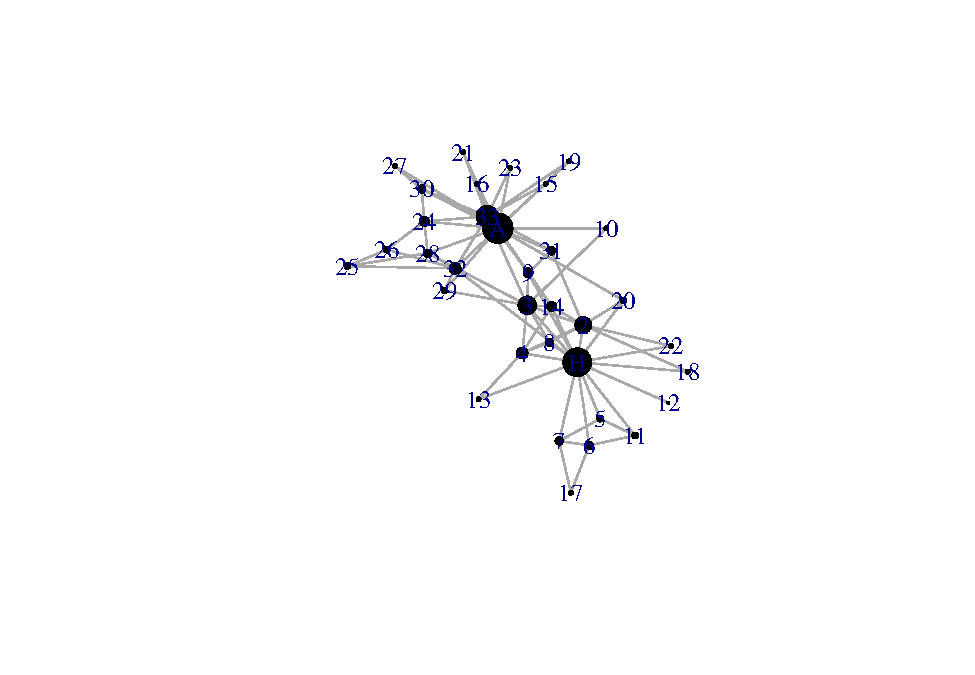
\includegraphics{bookdown-demo_files/figure-latex/unnamed-chunk-131-1.pdf}

\begin{Shaded}
\begin{Highlighting}[]
\CommentTok{\# what is the shortest path between nodes A and C?}
\FunctionTok{shortest\_paths}\NormalTok{(g\_w, }\AttributeTok{from =} \StringTok{"A"}\NormalTok{, }\AttributeTok{to =} \StringTok{"C"}\NormalTok{)}\SpecialCharTok{$}\NormalTok{vpath }\CommentTok{\# the shortest path is not A{-}B{-}C! }
\end{Highlighting}
\end{Shaded}

\begin{verbatim}
## [[1]]
## + 4/5 vertices, named, from 066e36b:
## [1] A D E C
\end{verbatim}

\begin{Shaded}
\begin{Highlighting}[]
\FunctionTok{shortest\_paths}\NormalTok{(g, }\AttributeTok{from =} \StringTok{"A"}\NormalTok{, }\AttributeTok{to =} \StringTok{"C"}\NormalTok{)}\SpecialCharTok{$}\NormalTok{vpath }\CommentTok{\# the shortest path is A{-}B{-}C! }
\end{Highlighting}
\end{Shaded}

\begin{verbatim}
## [[1]]
## + 3/5 vertices, named, from 066e36b:
## [1] A B C
\end{verbatim}

\begin{Shaded}
\begin{Highlighting}[]
\CommentTok{\# the reason is between bigger weights correspond to larger distances.}
\CommentTok{\# and hence longer paths }

\CommentTok{\# the shortest path is A{-}B{-}C after we invert the edge weights}
\FunctionTok{E}\NormalTok{(g\_w)}\SpecialCharTok{$}\NormalTok{weight }\OtherTok{\textless{}{-}} \DecValTok{1}\SpecialCharTok{/}\FunctionTok{c}\NormalTok{(}\DecValTok{2}\NormalTok{,}\DecValTok{1}\NormalTok{,}\DecValTok{2}\NormalTok{,}\DecValTok{1}\NormalTok{,}\DecValTok{1}\NormalTok{)}
\FunctionTok{shortest\_paths}\NormalTok{(g\_w, }\AttributeTok{from =} \StringTok{"A"}\NormalTok{, }\AttributeTok{to =} \StringTok{"C"}\NormalTok{)}\SpecialCharTok{$}\NormalTok{vpath }
\end{Highlighting}
\end{Shaded}

\begin{verbatim}
## [[1]]
## + 3/5 vertices, named, from 066e36b:
## [1] A B C
\end{verbatim}

To reiterate, if you have a weighted graph and you would like to compute weighted closeness centrality for your nodes AND your edge weights are already interpreted as \emph{distances} this is the pseudo R code that you need:

\begin{Shaded}
\begin{Highlighting}[]
\FunctionTok{closeness}\NormalTok{(network, }\AttributeTok{normalized =}\NormalTok{ T, }\AttributeTok{weights =} \FunctionTok{E}\NormalTok{(network)}\SpecialCharTok{$}\NormalTok{weight)}
\end{Highlighting}
\end{Shaded}

If your edge weights are interpreted as \emph{strengths}, then you need to mathematically ``flip'' or invert the edge weights.

\begin{Shaded}
\begin{Highlighting}[]
\CommentTok{\# take the inverse}
\FunctionTok{closeness}\NormalTok{(network, }\AttributeTok{normalized =}\NormalTok{ T, }\AttributeTok{weights =} \DecValTok{1}\SpecialCharTok{/}\FunctionTok{E}\NormalTok{(network)}\SpecialCharTok{$}\NormalTok{weight) }

\CommentTok{\# if your weights are Likert ratings, this code flips the scale around }
\FunctionTok{closeness}\NormalTok{(network, }\AttributeTok{normalized =}\NormalTok{ T, }
          \AttributeTok{weights =} \FunctionTok{abs}\NormalTok{(}\FunctionTok{E}\NormalTok{(network)}\SpecialCharTok{$}\NormalTok{weight }\SpecialCharTok{{-}}\NormalTok{ (}\FunctionTok{max}\NormalTok{(}\FunctionTok{E}\NormalTok{(network)}\SpecialCharTok{$}\NormalTok{weight) }\SpecialCharTok{+} \DecValTok{1}\NormalTok{))) }
\end{Highlighting}
\end{Shaded}

\subsection{Directed closeness centrality}\label{directed-closeness-centrality}

As shown in the example below for \emph{John A}, different closeness centrality values are returned depending on whether closeness centrality should be computed based on both incoming and outgoing edges (\texttt{mode\ =\ \textquotesingle{}all\textquotesingle{}}), incoming edges only (\texttt{mode\ =\ \textquotesingle{}in\textquotesingle{}}), or outgoing edges only (\texttt{mode\ =\ \textquotesingle{}out\textquotesingle{}}). Because \emph{John A} has an out-degree of 0 (see if you know how to verify this for yourself!), it has a closeness centrality of NaN when \texttt{mode\ =\ \textquotesingle{}out\textquotesingle{}} is specified.

\begin{Shaded}
\begin{Highlighting}[]
\FunctionTok{closeness}\NormalTok{(karate\_dw, }\AttributeTok{normalized =}\NormalTok{ T, }\AttributeTok{weights =} \ConstantTok{NA}\NormalTok{, }\AttributeTok{mode =} \StringTok{\textquotesingle{}all\textquotesingle{}}\NormalTok{, }\AttributeTok{vids =} \StringTok{\textquotesingle{}John A\textquotesingle{}}\NormalTok{)}
\end{Highlighting}
\end{Shaded}

\begin{verbatim}
## John A 
##   0.55
\end{verbatim}

\begin{Shaded}
\begin{Highlighting}[]
\FunctionTok{closeness}\NormalTok{(karate\_dw, }\AttributeTok{normalized =}\NormalTok{ T, }\AttributeTok{weights =} \ConstantTok{NA}\NormalTok{, }\AttributeTok{mode =} \StringTok{\textquotesingle{}in\textquotesingle{}}\NormalTok{, }\AttributeTok{vids =} \StringTok{\textquotesingle{}John A\textquotesingle{}}\NormalTok{)}
\end{Highlighting}
\end{Shaded}

\begin{verbatim}
##    John A 
## 0.7931034
\end{verbatim}

\begin{Shaded}
\begin{Highlighting}[]
\FunctionTok{closeness}\NormalTok{(karate\_dw, }\AttributeTok{normalized =}\NormalTok{ T, }\AttributeTok{weights =} \ConstantTok{NA}\NormalTok{, }\AttributeTok{mode =} \StringTok{\textquotesingle{}out\textquotesingle{}}\NormalTok{, }\AttributeTok{vids =} \StringTok{\textquotesingle{}John A\textquotesingle{}}\NormalTok{)}
\end{Highlighting}
\end{Shaded}

\begin{verbatim}
## John A 
##    NaN
\end{verbatim}

\section{Betweenness centrality}\label{betweenness-centrality}

\textbf{Betweenness centrality} is a measure of the degree to which nodes stand in between each other. A node with a high betweenness centrality is a node that is frequently found in the short paths of other pairs of nodes in the network. In contrast, a node with a low betweenness centrality is a node that is not usually found in the short paths of node pairs. Betweeenness can be viewed as an indicator of whether a node represents a ``bottleneck'' in the system.

The same considerations (i.e., about connected graphs, additional arguments for weighted and directed graphs, normalization, interpretation of weights as distances) from the closeness centrality section applies to betweenness centrality as well, because betweenness centrality also relies on the \texttt{shortest\_paths} function for its computation.

To get the betweenness centrality of all nodes in the network, try running the following code:

\begin{Shaded}
\begin{Highlighting}[]
\NormalTok{igraph}\SpecialCharTok{::}\FunctionTok{betweenness}\NormalTok{(karate\_dw, }\AttributeTok{normalized =}\NormalTok{ T) }\CommentTok{\# weights are automatically considered}
\end{Highlighting}
\end{Shaded}

\begin{verbatim}
##        Mr Hi      Actor 2      Actor 3      Actor 4      Actor 5      Actor 6      Actor 7      Actor 9     Actor 10     Actor 14     Actor 15     Actor 16     Actor 19     Actor 20     Actor 21     Actor 23 
## 0.0000000000 0.0021306818 0.0075757576 0.0040246212 0.0014204545 0.0000000000 0.0018939394 0.0016571970 0.0000000000 0.0023674242 0.0000000000 0.0000000000 0.0000000000 0.0000000000 0.0000000000 0.0000000000 
##     Actor 24     Actor 25     Actor 26     Actor 27     Actor 28     Actor 29     Actor 30     Actor 31     Actor 32     Actor 33      Actor 8     Actor 11     Actor 12     Actor 13     Actor 18     Actor 22 
## 0.0000000000 0.0000000000 0.0037878788 0.0000000000 0.0000000000 0.0018939394 0.0009469697 0.0026041667 0.0047348485 0.0056818182 0.0000000000 0.0000000000 0.0000000000 0.0000000000 0.0000000000 0.0000000000 
##     Actor 17       John A 
## 0.0000000000 0.0000000000
\end{verbatim}

\subsection{Weighted betweenness centrality}\label{weighted-betweenness-centrality}

If your network is weighted, weights are automatically included in the computation of betweenness centrality. If you prefer that edge weights are \emph{not} considered, include \texttt{weights\ =\ NA} in the argument. Notice that some of the values have changed depending on whether weights are considered or not.

If your network is unweighted, then weights are not considered by default.

\begin{Shaded}
\begin{Highlighting}[]
\NormalTok{igraph}\SpecialCharTok{::}\FunctionTok{betweenness}\NormalTok{(karate\_dw, }\AttributeTok{normalized =}\NormalTok{ T) }\CommentTok{\# weights are automatically considered}
\end{Highlighting}
\end{Shaded}

\begin{verbatim}
##        Mr Hi      Actor 2      Actor 3      Actor 4      Actor 5      Actor 6      Actor 7      Actor 9     Actor 10     Actor 14     Actor 15     Actor 16     Actor 19     Actor 20     Actor 21     Actor 23 
## 0.0000000000 0.0021306818 0.0075757576 0.0040246212 0.0014204545 0.0000000000 0.0018939394 0.0016571970 0.0000000000 0.0023674242 0.0000000000 0.0000000000 0.0000000000 0.0000000000 0.0000000000 0.0000000000 
##     Actor 24     Actor 25     Actor 26     Actor 27     Actor 28     Actor 29     Actor 30     Actor 31     Actor 32     Actor 33      Actor 8     Actor 11     Actor 12     Actor 13     Actor 18     Actor 22 
## 0.0000000000 0.0000000000 0.0037878788 0.0000000000 0.0000000000 0.0018939394 0.0009469697 0.0026041667 0.0047348485 0.0056818182 0.0000000000 0.0000000000 0.0000000000 0.0000000000 0.0000000000 0.0000000000 
##     Actor 17       John A 
## 0.0000000000 0.0000000000
\end{verbatim}

\begin{Shaded}
\begin{Highlighting}[]
\NormalTok{igraph}\SpecialCharTok{::}\FunctionTok{betweenness}\NormalTok{(karate\_dw, }\AttributeTok{normalized =}\NormalTok{ T, }\AttributeTok{weights =} \ConstantTok{NA}\NormalTok{) }\CommentTok{\# weights are ignored}
\end{Highlighting}
\end{Shaded}

\begin{verbatim}
##        Mr Hi      Actor 2      Actor 3      Actor 4      Actor 5      Actor 6      Actor 7      Actor 9     Actor 10     Actor 14     Actor 15     Actor 16     Actor 19     Actor 20     Actor 21     Actor 23 
## 0.0000000000 0.0004734848 0.0083648990 0.0018939394 0.0000000000 0.0004734848 0.0014204545 0.0021306818 0.0001578283 0.0016571970 0.0000000000 0.0000000000 0.0000000000 0.0005523990 0.0000000000 0.0000000000 
##     Actor 24     Actor 25     Actor 26     Actor 27     Actor 28     Actor 29     Actor 30     Actor 31     Actor 32     Actor 33      Actor 8     Actor 11     Actor 12     Actor 13     Actor 18     Actor 22 
## 0.0000000000 0.0000000000 0.0009469697 0.0000000000 0.0006313131 0.0020517677 0.0009469697 0.0007891414 0.0048137626 0.0001578283 0.0000000000 0.0000000000 0.0000000000 0.0000000000 0.0000000000 0.0000000000 
##     Actor 17       John A 
## 0.0000000000 0.0000000000
\end{verbatim}

\subsection{Directed betweenness centrality}\label{directed-betweenness-centrality}

As shown in the example below for \emph{John A}, different betweenness centrality values are returned depending on whether betweenness centrality should be computed by considering the directionality of the edges (\texttt{directed\ =\ TRUE}), or if edge direction should be ignored (\texttt{directed\ =\ FALSE}). Basically, if \texttt{directed\ =\ TRUE}, the shortest paths are only possible between node pairs where the edge directions are aligned (i.e., A-\textgreater B-\textgreater C), but if \texttt{directed\ =\ FALSE} then shortest paths are possible as long as there is an existing edge and direction of the edges is ignored.

\begin{Shaded}
\begin{Highlighting}[]
\NormalTok{igraph}\SpecialCharTok{::}\FunctionTok{betweenness}\NormalTok{(karate\_dw, }\AttributeTok{normalized =}\NormalTok{ T, }\AttributeTok{weights =} \ConstantTok{NA}\NormalTok{, }\AttributeTok{directed =} \ConstantTok{TRUE}\NormalTok{, }\AttributeTok{v =} \StringTok{\textquotesingle{}John A\textquotesingle{}}\NormalTok{)}
\end{Highlighting}
\end{Shaded}

\begin{verbatim}
## John A 
##      0
\end{verbatim}

\begin{Shaded}
\begin{Highlighting}[]
\NormalTok{igraph}\SpecialCharTok{::}\FunctionTok{betweenness}\NormalTok{(karate\_dw, }\AttributeTok{normalized =}\NormalTok{ T, }\AttributeTok{weights =} \ConstantTok{NA}\NormalTok{, }\AttributeTok{directed =} \ConstantTok{FALSE}\NormalTok{, }\AttributeTok{v =} \StringTok{\textquotesingle{}John A\textquotesingle{}}\NormalTok{)}
\end{Highlighting}
\end{Shaded}

\begin{verbatim}
##   John A 
## 0.304075
\end{verbatim}

Quick note: I've included \texttt{igraph::betweenness} to tell R to use the \texttt{betweenness} function from the \texttt{igraph} library and not the one from \texttt{influenceR} library (Chapter 12). This is important because sometimes different libraries have functions with the same name.

\section{Page Rank centrality}\label{page-rank-centrality}

\textbf{Page Rank centrality} is a centrality measure developed by Google to rank webpages (the historic paper describing the algorithm can be viewed \href{http://infolab.stanford.edu/~backrub/google.html}{here}). The general idea is that a random walker will traverse the network space and their paths are biased by the link connectivity structure of the network. The random walker restarts the walk after some time (simulating ``boredom'' of the surfer). The number of visits received by a node provides an indicator of its importance in the network. Intuitively, we expect that nodes have a high Page Rank score if there are many nodes that point to it, or if the nodes that point to it themselves have a high Page Rank score.

The \texttt{weights} and \texttt{directed} arguments can be adjusted depending on your graph type. It is important to note that the interpretation of edge weights here is that of ``connection strength'' (Reproduced from the \texttt{igraph} manual: ``This function interprets edge weights as connection strengths. In the random surfer model, an edge with a larger weight is more likely to be selected by the surfer.''). This is different from the ``distance'' interpretation of edge weights in the closeness and betweenness centralities sections.

To get the Page Rank centrality of all nodes in the network, try running the following code:

\begin{Shaded}
\begin{Highlighting}[]
\CommentTok{\# undirected, unweighted centralities }
\FunctionTok{page\_rank}\NormalTok{(}\AttributeTok{graph =}\NormalTok{ karate\_dw, }\AttributeTok{directed =}\NormalTok{ F, }\AttributeTok{weights =} \ConstantTok{NA}\NormalTok{)}\SpecialCharTok{$}\NormalTok{vector}
\end{Highlighting}
\end{Shaded}

\begin{verbatim}
##       Mr Hi     Actor 2     Actor 3     Actor 4     Actor 5     Actor 6     Actor 7     Actor 9    Actor 10    Actor 14    Actor 15    Actor 16    Actor 19    Actor 20    Actor 21    Actor 23    Actor 24    Actor 25 
## 0.096997285 0.052876924 0.057078509 0.035859858 0.021977952 0.029111155 0.029111155 0.029766056 0.014309397 0.029536456 0.014535994 0.014535994 0.014535994 0.019604636 0.014535994 0.014535994 0.031522515 0.021076034 
##    Actor 26    Actor 27    Actor 28    Actor 29    Actor 30    Actor 31    Actor 32    Actor 33     Actor 8    Actor 11    Actor 12    Actor 13    Actor 18    Actor 22    Actor 17      John A 
## 0.021006197 0.015044038 0.025639767 0.019573459 0.026288538 0.024590155 0.037158087 0.071693226 0.024490497 0.021977952 0.009564745 0.014644892 0.014558677 0.014558677 0.016784005 0.100919182
\end{verbatim}

\begin{Shaded}
\begin{Highlighting}[]
\CommentTok{\# directed, weighted centralities (weights used by default)}
\FunctionTok{page\_rank}\NormalTok{(}\AttributeTok{graph =}\NormalTok{ karate\_dw, }\AttributeTok{directed =}\NormalTok{ T)}\SpecialCharTok{$}\NormalTok{vector}
\end{Highlighting}
\end{Shaded}

\begin{verbatim}
##      Mr Hi    Actor 2    Actor 3    Actor 4    Actor 5    Actor 6    Actor 7    Actor 9   Actor 10   Actor 14   Actor 15   Actor 16   Actor 19   Actor 20   Actor 21   Actor 23   Actor 24   Actor 25   Actor 26 
## 0.01523537 0.01552315 0.01938528 0.01886916 0.01581093 0.01667427 0.03091729 0.01884496 0.01729506 0.02746170 0.01523537 0.01523537 0.01523537 0.01701045 0.01523537 0.01523537 0.01523537 0.01523537 0.01935585 
##   Actor 27   Actor 28   Actor 29   Actor 30   Actor 31   Actor 32   Actor 33    Actor 8   Actor 11   Actor 12   Actor 13   Actor 18   Actor 22   Actor 17     John A 
## 0.01523537 0.02484945 0.01798162 0.02141609 0.01939474 0.04512689 0.08402038 0.02351277 0.02484309 0.01552315 0.01988203 0.01880972 0.01672267 0.04556454 0.26808640
\end{verbatim}

\begin{Shaded}
\begin{Highlighting}[]
\CommentTok{\# notice we include the "$vector" after the function because the function outputs}
\CommentTok{\# a list object, and we only want the part of the object that contains the }
\CommentTok{\# centrality values for the individual nodes }
\end{Highlighting}
\end{Shaded}

\section{Other forms of node centrality}\label{other-forms-of-node-centrality}

\texttt{igraph} is also able to compute the following node centrality scores:

\begin{itemize}
\tightlist
\item
  \href{https://igraph.org/r/doc/authority_score.html}{authority score}
\item
  \href{https://igraph.org/r/doc/eigen_centrality.html}{eigenvector centrality}; directed generalization is \href{https://igraph.org/r/doc/alpha_centrality.html}{alpha centrality}
\item
  \href{https://igraph.org/r/doc/harmonic_centrality.html}{harmonic centrality}
\item
  \href{https://igraph.org/r/doc/hub_score.html}{hub centrality}
\item
  \href{https://igraph.org/r/doc/power_centrality.html}{power centrality}
\end{itemize}

If you interested to learn about these the links to the \texttt{igraph} documentation are included above. \{May be further discussed in later versions of the book.\}

\section{Exporting node centrality measures for data analysis}\label{exporting-node-centrality-measures-for-data-analysis}

As you can see from this chapter, it is fairly straightforward to obtain node centrality measures--you need to know which functions to use, and think about whether you want a variant of the measure that reflects properties of the network that are important for your research (e.g., directedness and weightedness of the edges). However, printing out the values in the Console is unwieldy, and makes it quite difficult to manipulate and analyze this information.

Below is a code chunk that you should be able to easily edit to extract the measures that you want for all nodes in a given network. It creates a data frame containing each centrality measure in a separate column and node names in another column. You can add more or fewer centrality measures in the data frame. Then you analyze the data frame object as per normal (e.g., are degree and local clustering coefficient of nodes positively correlated in this network?) or export the data frame so that you can merge it with other measures (e.g., gender of each person) and conduct statistical tests in another software (e.g., on average, do males have a higher closeness centrality than females?).

\begin{Shaded}
\begin{Highlighting}[]
\NormalTok{node\_centrality\_data }\OtherTok{\textless{}{-}} \FunctionTok{data.frame}\NormalTok{(}
    \AttributeTok{degree =} \FunctionTok{degree}\NormalTok{(karate\_dw, }\AttributeTok{mode =} \StringTok{\textquotesingle{}all\textquotesingle{}}\NormalTok{), }\CommentTok{\# column\_name = centrality function }
    \AttributeTok{out\_strength =} \FunctionTok{strength}\NormalTok{(karate\_dw, }\AttributeTok{mode =} \StringTok{\textquotesingle{}out\textquotesingle{}}\NormalTok{),}
    \AttributeTok{uu\_closeness =} \FunctionTok{closeness}\NormalTok{(karate\_dw, }\AttributeTok{normalized =} \ConstantTok{TRUE}\NormalTok{, }\AttributeTok{mode =} \StringTok{\textquotesingle{}all\textquotesingle{}}\NormalTok{, }\AttributeTok{weights =} \ConstantTok{NA}\NormalTok{)}
\NormalTok{    )}

\FunctionTok{write.csv}\NormalTok{(node\_centrality\_data, }\AttributeTok{file =} \StringTok{\textquotesingle{}results.csv\textquotesingle{}}\NormalTok{)}
\end{Highlighting}
\end{Shaded}

\section{Exercise}\label{exercise-5}

Your task is to:

\begin{enumerate}
\def\labelenumi{\arabic{enumi}.}
\tightlist
\item
  Load the famous \href{https://en.wikipedia.org/wiki/Krackhardt_kite_graph}{Krackhardt's Kite} network from the \texttt{igraphdata} library using the following code:
\end{enumerate}

\begin{Shaded}
\begin{Highlighting}[]
\FunctionTok{library}\NormalTok{(igraphdata) }\CommentTok{\# have you downloaded the package? }

\FunctionTok{data}\NormalTok{(}\StringTok{"kite"}\NormalTok{) }\CommentTok{\# you should see a kite object appear in your Environment}
\end{Highlighting}
\end{Shaded}

\begin{enumerate}
\def\labelenumi{\arabic{enumi}.}
\setcounter{enumi}{1}
\tightlist
\item
  Answer the following questions:
\end{enumerate}

\begin{itemize}
\item
  How many nodes and edges does the network have?
\item
  What type of edges does the network have?
\item
  Find out which node(s) has:

  \begin{itemize}
  \tightlist
  \item
    the highest/lowest degree in the network?
  \item
    the highest/lowest local clustering coefficient?
  \item
    the highest/lowest betweenness centrality?
  \item
    the highest/lowest closeness centrality?
  \item
    the highest/lowest Page Rank centrality?
  \end{itemize}
\end{itemize}

\begin{enumerate}
\def\labelenumi{\arabic{enumi}.}
\setcounter{enumi}{2}
\item
  Save the node-level measures as a \texttt{.csv} file and open it in a spreadsheet program of your choice.
\item
  Do the same nodes have the highest degree, closeness, and betweenness centrality scores in this network? Try plotting the network and explain why different nodes have the highest scores on these centrality measures.
\end{enumerate}

\chapter{Chapter 8: Meso-level network measures}\label{ch8}

A common feature of many real-world networks is that they have robust community structure. Nodes are considered to be part of the same community if the density of connections among those nodes is relatively higher than the density of connections between nodes from different communities (Newman, 2006).

\textbf{Modularity}, \emph{Q}, is a measure of the density of links inside communities in relation to the density of links between communities (Fortunato, 2010). Networks with higher \emph{Q} are said to show strong evidence of community structure.

\section{How do network scientists ``find'' communities in networks?}\label{how-do-network-scientists-find-communities-in-networks}

Many community detection methods have been developed by network scientists to detect communities in networks. Each differs in their implementation, and reflects the creator's implicit definition of what is a community. In this section we will explore just 4 of these methods.

If you are interested to learn more about community detection, check out Fortunato (2010) who provided a comprehensive comparison of various community detection techniques.

In this section we will use the undirected, unweighted version of the karate network from Chapter 4 for demonstration.

\begin{Shaded}
\begin{Highlighting}[]
\NormalTok{karate\_el }\OtherTok{\textless{}{-}} \FunctionTok{read.csv}\NormalTok{(}\StringTok{\textquotesingle{}data/karate\_el.csv\textquotesingle{}}\NormalTok{, }\AttributeTok{header =} \ConstantTok{FALSE}\NormalTok{)}

\NormalTok{karate\_uu }\OtherTok{\textless{}{-}} \FunctionTok{graph\_from\_data\_frame}\NormalTok{(karate\_el, }\AttributeTok{directed =} \ConstantTok{FALSE}\NormalTok{)}

\FunctionTok{summary}\NormalTok{(karate\_uu)}
\end{Highlighting}
\end{Shaded}

\begin{verbatim}
## IGRAPH 5acc868 UN-- 34 78 -- 
## + attr: name (v/c)
\end{verbatim}

As you will see in the rest of this chapter, the template for conducting a community detection analysis is identical across the four methods. \texttt{igraph} contains additional community detection algorithms not covered in this chapter, but you should be able to generalize the application of these algorithms based on the code provided below. Generally, community detection algorithms have in-built default parameters that are used to optimize performance. At the completion of the method, it returns the communities (i.e., how the individual nodes are grouped), and the modularity score based on this final grouping.

\section{Edge betweenness (``divisive method'')}\label{edge-betweenness-divisive-method}

The core idea behind the edge betweenness community detection method is that edges connecting separate communities tend to have high edge betweenness as all the shortest paths from one community to another must necessarily traverse through these edges.

The algorithm works by calculating the edge betweenness of all edges of the graph, and then removing the edge with the highest edge betweenness score. It recalculates the edge betweenness of remaining edges and again removes the one with the highest score. This repeats until modularity cannot be improved further.

Because there may be random components in the community detection algorithm, it is a good idea to use \texttt{set.seed} to ensure that your results are reproducible. Usually the algorithm is repeated several times, and the results are compared across runs. For now we will just run the algorithm once and return to this point at the end of this section.

For the edge betweenness method, we use the \texttt{cluster\_edge\_betweenness} function. Functions that begin with \texttt{cluster\_} are community detection methods in \texttt{igraph}. The outputs of the community detection are saved into the \texttt{karate\_edge} object.

\begin{Shaded}
\begin{Highlighting}[]
\FunctionTok{set.seed}\NormalTok{(}\DecValTok{1}\NormalTok{)}

\NormalTok{karate\_edge }\OtherTok{\textless{}{-}} \FunctionTok{cluster\_edge\_betweenness}\NormalTok{(karate\_uu)}
\end{Highlighting}
\end{Shaded}

Normally, we wish to know at least these 3 things from the community detection results, which we can easily retrieve from the \texttt{karate\_edge} object:

\begin{enumerate}
\def\labelenumi{\arabic{enumi}.}
\tightlist
\item
  The community membership of each node in the network (i.e., which nodes belong to the same community?). In the code below, this is merged with the node names and only the first 10 nodes are shown. It would be straightforward to save and export this information for further analyses; see the commented code below.
\item
  We also want to know how nodes are distributed across the communities. By using the \texttt{table} function we get a count of the community labels. Here, we can see that there are a total of 5 communities, the largest one consisting of 12 nodes (community 4) and the smallest one consisting of a single node (community 5).
\item
  The modularity of the final community grouping, which gives us a sense of the quality of partitions retrieved by the algorithm. Here, \emph{Q} is 0.401.
\end{enumerate}

\begin{Shaded}
\begin{Highlighting}[]
\CommentTok{\# 1. membership of nodes in each community }
\FunctionTok{data.frame}\NormalTok{(}\AttributeTok{node =} \FunctionTok{V}\NormalTok{(karate\_uu)}\SpecialCharTok{$}\NormalTok{name, }\AttributeTok{community =}\NormalTok{ karate\_edge}\SpecialCharTok{$}\NormalTok{membership) }\SpecialCharTok{|\textgreater{}} 
  \FunctionTok{head}\NormalTok{(}\DecValTok{10}\NormalTok{) }\CommentTok{\# view the first 10}
\end{Highlighting}
\end{Shaded}

\begin{verbatim}
##        node community
## 1     Mr Hi         1
## 2   Actor 2         1
## 3   Actor 3         2
## 4   Actor 4         1
## 5   Actor 5         3
## 6   Actor 6         3
## 7   Actor 7         3
## 8   Actor 9         4
## 9  Actor 10         5
## 10 Actor 14         1
\end{verbatim}

\begin{Shaded}
\begin{Highlighting}[]
\DocumentationTok{\#\#\# saving the results }
\CommentTok{\# results \textless{}{-} data.frame(node = V(karate\_uu)$name, community = karate\_edge$membership)}
\CommentTok{\# write.csv(results, file = \textquotesingle{}results.csv\textquotesingle{})}

\CommentTok{\# 2. distribution of nodes across communities}
\FunctionTok{table}\NormalTok{(karate\_edge}\SpecialCharTok{$}\NormalTok{membership) }
\end{Highlighting}
\end{Shaded}

\begin{verbatim}
## 
##  1  2  3  4  5 
## 10  6  5 12  1
\end{verbatim}

\begin{Shaded}
\begin{Highlighting}[]
\CommentTok{\# 3. modularity of the network }
\FunctionTok{modularity}\NormalTok{(karate\_edge)  }
\end{Highlighting}
\end{Shaded}

\begin{verbatim}
## [1] 0.4012985
\end{verbatim}

In the subsequent sections, you will notice that the structure of the code/output is identical, except for the specific community detection function used.

\section{Louvain method (``greedy, maximization method'')}\label{louvain-method-greedy-maximization-method}

The core idea behind the Louvain community detection method is that communities are essentially ``mergers'' of small communities (Blondel et al., 2008), reflecting the self-similar nature of complex networks.

\begin{enumerate}
\def\labelenumi{\arabic{enumi}.}
\item
  Each node is assigned to one community such that there are as many communities as there are nodes. Then remove node \emph{i} from its community and place it in the community of the neighbor which yields the greatest gain in modularity. Repeat for all nodes in the network.
\item
  A new network is built where nodes are the communities found in the previous phase. Repeat Step 1.
\item
  Repeat Step 1 and 2 until it is not possible to further increase the value of \emph{Q}.
\end{enumerate}

For the Louvain method, we use the \texttt{cluster\_louvain} function. The outputs of the community detection are saved into the \texttt{karate\_louvain} object.

\begin{Shaded}
\begin{Highlighting}[]
\FunctionTok{set.seed}\NormalTok{(}\DecValTok{1}\NormalTok{)}

\NormalTok{karate\_louvain }\OtherTok{\textless{}{-}} \FunctionTok{cluster\_louvain}\NormalTok{(karate\_uu)}

\CommentTok{\# 1. membership of nodes in each community }
\FunctionTok{data.frame}\NormalTok{(}\AttributeTok{node =} \FunctionTok{V}\NormalTok{(karate\_uu)}\SpecialCharTok{$}\NormalTok{name, }\AttributeTok{community =}\NormalTok{ karate\_louvain}\SpecialCharTok{$}\NormalTok{membership) }\SpecialCharTok{|\textgreater{}} 
  \FunctionTok{head}\NormalTok{(}\DecValTok{10}\NormalTok{) }\CommentTok{\# view the first 10}
\end{Highlighting}
\end{Shaded}

\begin{verbatim}
##        node community
## 1     Mr Hi         1
## 2   Actor 2         1
## 3   Actor 3         1
## 4   Actor 4         1
## 5   Actor 5         2
## 6   Actor 6         2
## 7   Actor 7         2
## 8   Actor 9         3
## 9  Actor 10         1
## 10 Actor 14         1
\end{verbatim}

\begin{Shaded}
\begin{Highlighting}[]
\CommentTok{\# 2. distribution of nodes across communities}
\FunctionTok{table}\NormalTok{(karate\_louvain}\SpecialCharTok{$}\NormalTok{membership) }
\end{Highlighting}
\end{Shaded}

\begin{verbatim}
## 
##  1  2  3  4 
## 12  5 11  6
\end{verbatim}

\begin{Shaded}
\begin{Highlighting}[]
\CommentTok{\# 3. modularity of the network }
\FunctionTok{modularity}\NormalTok{(karate\_louvain)  }
\end{Highlighting}
\end{Shaded}

\begin{verbatim}
## [1] 0.4188034
\end{verbatim}

Notice that the Louvain method returned 4 communities ranging in size from 5 to 12, with a \emph{Q} of 0.419.

\section{Random walker (``dynamic method'')}\label{random-walker-dynamic-method}

The core idea behind the random walker community detection method is that if there are communities in the network, a random walker will tend to spend more time inside the community than outside.

The Walktrap algorithm groups nodes together based on the similarities of the paths taken by the random walker starting from that node. The idea is to merge sets of vertices that have low ``distance'' from each other.

For the random walker method, we use the \texttt{cluster\_walktrap} function. The outputs of the community detection are saved into the \texttt{karate\_walktrap} object.

\begin{Shaded}
\begin{Highlighting}[]
\FunctionTok{set.seed}\NormalTok{(}\DecValTok{1}\NormalTok{)}

\NormalTok{karate\_walktrap }\OtherTok{\textless{}{-}} \FunctionTok{cluster\_walktrap}\NormalTok{(karate\_uu)}

\CommentTok{\# 1. membership of nodes in each community }
\FunctionTok{data.frame}\NormalTok{(}\AttributeTok{node =} \FunctionTok{V}\NormalTok{(karate\_uu)}\SpecialCharTok{$}\NormalTok{name, }\AttributeTok{community =}\NormalTok{ karate\_walktrap}\SpecialCharTok{$}\NormalTok{membership) }\SpecialCharTok{|\textgreater{}} 
  \FunctionTok{head}\NormalTok{(}\DecValTok{10}\NormalTok{) }\CommentTok{\# view the first 10}
\end{Highlighting}
\end{Shaded}

\begin{verbatim}
##        node community
## 1     Mr Hi         1
## 2   Actor 2         1
## 3   Actor 3         2
## 4   Actor 4         1
## 5   Actor 5         5
## 6   Actor 6         5
## 7   Actor 7         5
## 8   Actor 9         2
## 9  Actor 10         2
## 10 Actor 14         2
\end{verbatim}

\begin{Shaded}
\begin{Highlighting}[]
\CommentTok{\# 2. distribution of nodes across communities}
\FunctionTok{table}\NormalTok{(karate\_walktrap}\SpecialCharTok{$}\NormalTok{membership) }
\end{Highlighting}
\end{Shaded}

\begin{verbatim}
## 
## 1 2 3 4 5 
## 9 7 9 4 5
\end{verbatim}

\begin{Shaded}
\begin{Highlighting}[]
\CommentTok{\# 3. modularity of the network }
\FunctionTok{modularity}\NormalTok{(karate\_walktrap)  }
\end{Highlighting}
\end{Shaded}

\begin{verbatim}
## [1] 0.3532216
\end{verbatim}

Notice that the random walker method returned 5 communities ranging in size from 5 to 9, with a \emph{Q} of 0.353.

\section{Infomap (``information-theoretic method'')}\label{infomap-information-theoretic-method}

The core idea behind the Infomap community detection method is to leverage on information-theoretic methods to ``describe'' the information flow of the entire system (based on random walks).

The Infomap algorithm attempts to describe the random walker's trajectory using the fewest number of ``bits'' of information. Communities are groups of nodes that receive new ``names'' during the compression process.

For the Infomap method, we use the \texttt{cluster\_infomap} function. The outputs of the community detection are saved into the \texttt{karate\_infomap} object.

\begin{Shaded}
\begin{Highlighting}[]
\FunctionTok{set.seed}\NormalTok{(}\DecValTok{1}\NormalTok{)}

\NormalTok{karate\_infomap }\OtherTok{\textless{}{-}} \FunctionTok{cluster\_infomap}\NormalTok{(karate\_uu)}

\CommentTok{\# 1. membership of nodes in each community }
\FunctionTok{data.frame}\NormalTok{(}\AttributeTok{node =} \FunctionTok{V}\NormalTok{(karate\_uu)}\SpecialCharTok{$}\NormalTok{name, }\AttributeTok{community =}\NormalTok{ karate\_infomap}\SpecialCharTok{$}\NormalTok{membership) }\SpecialCharTok{|\textgreater{}} 
  \FunctionTok{head}\NormalTok{(}\DecValTok{10}\NormalTok{) }\CommentTok{\# view the first 10}
\end{Highlighting}
\end{Shaded}

\begin{verbatim}
##        node community
## 1     Mr Hi         1
## 2   Actor 2         1
## 3   Actor 3         1
## 4   Actor 4         1
## 5   Actor 5         2
## 6   Actor 6         2
## 7   Actor 7         2
## 8   Actor 9         3
## 9  Actor 10         1
## 10 Actor 14         1
\end{verbatim}

\begin{Shaded}
\begin{Highlighting}[]
\CommentTok{\# 2. distribution of nodes across communities}
\FunctionTok{table}\NormalTok{(karate\_infomap}\SpecialCharTok{$}\NormalTok{membership) }
\end{Highlighting}
\end{Shaded}

\begin{verbatim}
## 
##  1  2  3 
## 12  5 17
\end{verbatim}

\begin{Shaded}
\begin{Highlighting}[]
\CommentTok{\# 3. modularity of the network }
\FunctionTok{modularity}\NormalTok{(karate\_infomap)  }
\end{Highlighting}
\end{Shaded}

\begin{verbatim}
## [1] 0.4020381
\end{verbatim}

Notice that the Infomap method returned 3 communities ranging in size from 5 to 17, with a \emph{Q} of 0.402.

\section{Comparison of methods}\label{comparison-of-methods}

Fortunato (2010) conducted a comprehensive comparison of community detection techniques. Generally, Rosvall \& Bergstorm's Infomap and Blondel et al.'s greedy modularity maximization method performed the best. Both also were relatively fast algorithms that were efficient for large networks.

The code below illustrates the similarities and differences in the results of the various community detection methods.

\subsection{Comparing modularity}\label{comparing-modularity}

In this example, the Louvain method yielded community groupings that led to the highest \emph{Q} score of 0.419, whereas the Walktrap method yielded the lowest \emph{Q} score of 0.353. Overall, there is moderately strong evidence of community structure in the karate network with modularity scores approximating \textasciitilde0.40 across the four community detection methods used.

\begin{Shaded}
\begin{Highlighting}[]
\FunctionTok{modularity}\NormalTok{(karate\_edge)}
\end{Highlighting}
\end{Shaded}

\begin{verbatim}
## [1] 0.4012985
\end{verbatim}

\begin{Shaded}
\begin{Highlighting}[]
\FunctionTok{modularity}\NormalTok{(karate\_louvain)}
\end{Highlighting}
\end{Shaded}

\begin{verbatim}
## [1] 0.4188034
\end{verbatim}

\begin{Shaded}
\begin{Highlighting}[]
\FunctionTok{modularity}\NormalTok{(karate\_walktrap)}
\end{Highlighting}
\end{Shaded}

\begin{verbatim}
## [1] 0.3532216
\end{verbatim}

\begin{Shaded}
\begin{Highlighting}[]
\FunctionTok{modularity}\NormalTok{(karate\_infomap)}
\end{Highlighting}
\end{Shaded}

\begin{verbatim}
## [1] 0.4020381
\end{verbatim}

\subsection{Comparing community membership}\label{comparing-community-membership}

The code below provides the following visualization that compares how different methods are grouping nodes into communities.

\begin{Shaded}
\begin{Highlighting}[]
\FunctionTok{par}\NormalTok{(}\AttributeTok{mar=}\FunctionTok{c}\NormalTok{(}\DecValTok{0}\NormalTok{,}\DecValTok{0}\NormalTok{,}\DecValTok{0}\NormalTok{,}\DecValTok{0}\NormalTok{)}\SpecialCharTok{+}\NormalTok{.}\DecValTok{6}\NormalTok{, }\AttributeTok{mfrow =} \FunctionTok{c}\NormalTok{(}\DecValTok{2}\NormalTok{,}\DecValTok{2}\NormalTok{)) }\CommentTok{\# reduce margins and plot both networks together}

\FunctionTok{set.seed}\NormalTok{(}\DecValTok{1}\NormalTok{)}
\NormalTok{fixed\_l }\OtherTok{\textless{}{-}} \FunctionTok{layout\_with\_fr}\NormalTok{(karate\_uu) }\CommentTok{\# to fix node layout across plots }

\FunctionTok{plot}\NormalTok{(karate\_edge, karate\_uu, }\AttributeTok{layout =}\NormalTok{ fixed\_l, }\AttributeTok{main =} \StringTok{\textquotesingle{}edge betweenness\textquotesingle{}}\NormalTok{, }\AttributeTok{vertex.label =} \ConstantTok{NA}\NormalTok{)}
\FunctionTok{plot}\NormalTok{(karate\_louvain, karate\_uu, }\AttributeTok{layout =}\NormalTok{ fixed\_l, }\AttributeTok{main =} \StringTok{\textquotesingle{}Louvain\textquotesingle{}}\NormalTok{, }\AttributeTok{vertex.label =} \ConstantTok{NA}\NormalTok{)}
\FunctionTok{plot}\NormalTok{(karate\_walktrap, karate\_uu, }\AttributeTok{layout =}\NormalTok{ fixed\_l, }\AttributeTok{main =} \StringTok{\textquotesingle{}Walktrap\textquotesingle{}}\NormalTok{, }\AttributeTok{vertex.label =} \ConstantTok{NA}\NormalTok{)}
\FunctionTok{plot}\NormalTok{(karate\_infomap, karate\_uu, }\AttributeTok{layout =}\NormalTok{ fixed\_l, }\AttributeTok{main =} \StringTok{\textquotesingle{}Infomap\textquotesingle{}}\NormalTok{, }\AttributeTok{vertex.label =} \ConstantTok{NA}\NormalTok{)}
\end{Highlighting}
\end{Shaded}

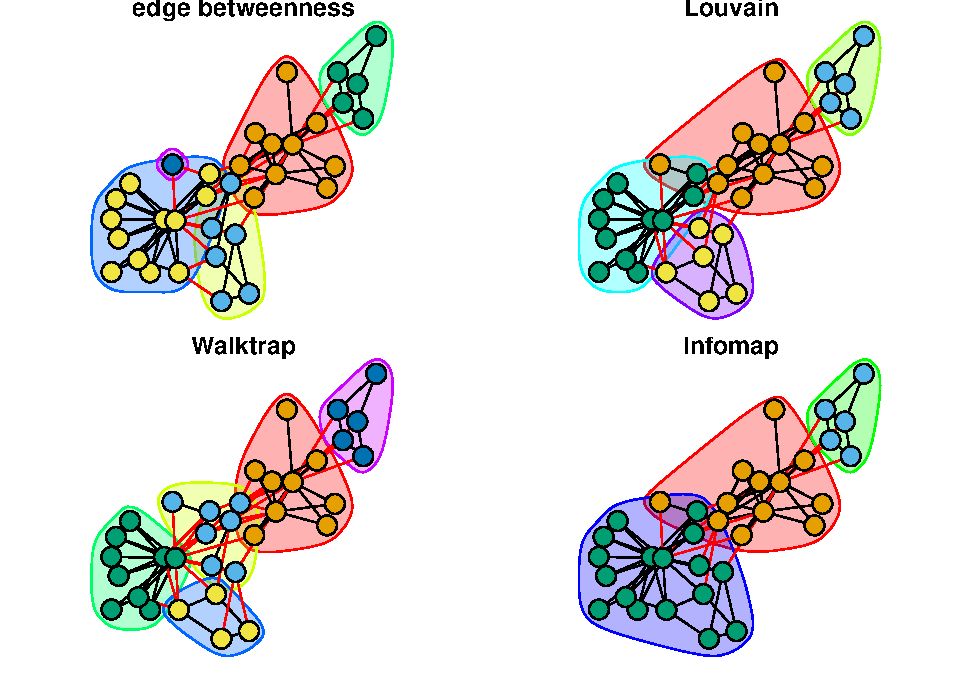
\includegraphics{bookdown-demo_files/figure-latex/unnamed-chunk-148-1.pdf}

More formally, we can make use of statistical methods such as the Fleiss' Kappa test to quantify the extent to which the groupings are consistent across the 4 methods.

\begin{Shaded}
\begin{Highlighting}[]
\CommentTok{\# first, compile the community membership results from all methods }
\NormalTok{compare\_membership }\OtherTok{\textless{}{-}} \FunctionTok{data.frame}\NormalTok{(}
  \AttributeTok{edge =}\NormalTok{ karate\_edge}\SpecialCharTok{$}\NormalTok{membership,}
  \AttributeTok{louvain =}\NormalTok{ karate\_louvain}\SpecialCharTok{$}\NormalTok{membership,}
  \AttributeTok{walktrap =}\NormalTok{ karate\_walktrap}\SpecialCharTok{$}\NormalTok{membership,}
  \AttributeTok{infomap =}\NormalTok{ karate\_infomap}\SpecialCharTok{$}\NormalTok{membership}
\NormalTok{)}

\CommentTok{\# compute consistency that two nodes tend to be found in the same cluster }
\FunctionTok{library}\NormalTok{(irr) }\CommentTok{\# we need this library for the kappa test of interrater agreement }
\end{Highlighting}
\end{Shaded}

\begin{verbatim}
## Loading required package: lpSolve
\end{verbatim}

\begin{Shaded}
\begin{Highlighting}[]
\FunctionTok{kappam.fleiss}\NormalTok{(compare\_membership)}
\end{Highlighting}
\end{Shaded}

\begin{verbatim}
##  Fleiss' Kappa for m Raters
## 
##  Subjects = 34 
##    Raters = 4 
##     Kappa = 0.332 
## 
##         z = 8.46 
##   p-value = 0
\end{verbatim}

Although the Kappa test is significant at \emph{p} \textless{} .05, indicating that the groupings are more consistent than expected from chance, the Kappa value of 0.332 is relatively low. This suggests that the community detection methods are returning similar but also somewhat different results in the community membership of individual nodes.

\{Note: You may need to relabel so that `1' corresponds to most popular category, etc.\}

\section{Things to note}\label{things-to-note}

Before ending this chapter it is worth highlighting the following.

\subsection{Weighted and directed graphs}\label{weighted-and-directed-graphs}

Some of the community detection methods listed above can make use of weighted and directed information in the community detection process; please refer to the documentation for details. Typically, you would need to modify the arguments in the \texttt{cluster\_} function to indicate that edge weights and direction should be considered. Please note that the interpretation of edge weights as distances or connection strength (see Chapter 7) can differ depending on the community detection method. Again, refer to the documentation for more information.

\subsection{Networks with multiple components}\label{networks-with-multiple-components}

As discussed in Chapter 6, not all nodes in the network necessarily forms a single connected component. In networks containing multiple network components, it is very likely that nodes in the smaller components are grouped together as a community in any community detection method. This is because doing so naturally optimizes modularity; hence, communities would never contain nodes that come from different components. It may make more sense to focus the community detection on the largest connected component of the network.

\subsection{Calculating modularity for self-defined communities}\label{calculating-modularity-for-self-defined-communities}

It is possible to compute modularity based on pre-specified communities. For instance, you may have prior information on the subgroups that each node in the network belongs to (i.e., community labels that are extrinsic to the network structure; e.g., student interest groups or majors) and you want to see how those groupings correspond to the connectivity structure.

If the modularity of those labels are quite high and comparable to the community detection results, it would suggest that nodes that belong to the same extrinsic group also have relatively higher density of connections internally, relative to the density of connections across different groups.

In the toy example below, I provided ``made-up'' groups to the karate network through the node-attribute ``suburb''. Because these labels were randomly generated, we would expect modularity computed based on these groups to be very low or close to zero.

\begin{Shaded}
\begin{Highlighting}[]
\CommentTok{\# let\textquotesingle{}s assume we have information about the suburb that each karate member lives in }
\FunctionTok{V}\NormalTok{(karate\_uu)}\SpecialCharTok{$}\NormalTok{suburb }\OtherTok{\textless{}{-}} \FunctionTok{sample}\NormalTok{(}\DecValTok{1}\SpecialCharTok{:}\DecValTok{5}\NormalTok{, }\FunctionTok{gorder}\NormalTok{(karate\_uu), }\AttributeTok{replace =} \ConstantTok{TRUE}\NormalTok{)}

\FunctionTok{modularity}\NormalTok{(karate\_uu, }\AttributeTok{membership =} \FunctionTok{V}\NormalTok{(karate\_uu)}\SpecialCharTok{$}\NormalTok{suburb) }\CommentTok{\# specify your own labels }
\end{Highlighting}
\end{Shaded}

\begin{verbatim}
## [1] -0.06402038
\end{verbatim}

\subsection{Comparing different runs}\label{comparing-different-runs}

As mentioned in the introduction of this chapter, you can get slightly different results even when re-running the same community detection method on the same network (assuming that you did not initially set a stable random seed). It is a good idea to repeat this multiple times to check if your results are generally consistent. The code below shows you how to run the algorithm multiple times and save the outputs into a list object that you can later investigate further.

As you can see there are minor variations in the modularity scores for each instance, and the very high Kappa score of 0.95 indicates highly consistent communities across runs.

\begin{Shaded}
\begin{Highlighting}[]
\NormalTok{cluster\_results }\OtherTok{\textless{}{-}} \FunctionTok{list}\NormalTok{()}

\ControlFlowTok{for}\NormalTok{(i }\ControlFlowTok{in} \DecValTok{1}\SpecialCharTok{:}\DecValTok{5}\NormalTok{) \{ }\CommentTok{\# change 5 to a different number if you want more runs }
  \FunctionTok{set.seed}\NormalTok{(i)}
  
\NormalTok{  cluster\_results[[i]] }\OtherTok{\textless{}{-}} \FunctionTok{cluster\_louvain}\NormalTok{(karate\_uu)}
\NormalTok{\}}

\CommentTok{\# compare Q}
\FunctionTok{sapply}\NormalTok{(cluster\_results, modularity)}
\end{Highlighting}
\end{Shaded}

\begin{verbatim}
## [1] 0.4188034 0.4188034 0.4188034 0.4155983 0.4155983
\end{verbatim}

\begin{Shaded}
\begin{Highlighting}[]
\CommentTok{\# compare consistency of membership }
\CommentTok{\# first, compile the community membership results from all runs into a single df}
\NormalTok{df1 }\OtherTok{\textless{}{-}} \FunctionTok{lapply}\NormalTok{(cluster\_results, }\ControlFlowTok{function}\NormalTok{(x) x}\SpecialCharTok{$}\NormalTok{membership)}
\NormalTok{df1\_merged }\OtherTok{\textless{}{-}} \FunctionTok{do.call}\NormalTok{(cbind, df1)}

\FunctionTok{kappam.fleiss}\NormalTok{(df1\_merged)}
\end{Highlighting}
\end{Shaded}

\begin{verbatim}
##  Fleiss' Kappa for m Raters
## 
##  Subjects = 34 
##    Raters = 5 
##     Kappa = 0.95 
## 
##         z = 28.6 
##   p-value = 0
\end{verbatim}

\subsection{Other community detection methods}\label{other-community-detection-methods}

Several other community detection methods can be implemented in \texttt{igraph}:

\begin{itemize}
\tightlist
\item
  \href{https://igraph.org/r/doc/cluster_fast_greedy.html}{cluster\_fast\_greedy} - fast greedy modularity optimization algorithm
\item
  \href{https://igraph.org/r/doc/cluster_fluid_communities.html}{cluster\_fluid\_communities} - community detection algorithm based on interacting fluids
\item
  \href{https://igraph.org/r/doc/cluster_label_prop.html}{cluster\_label\_prop} - community detection based on majority voting of label in the neighborhood of the vertex
\item
  \href{https://igraph.org/r/doc/cluster_leading_eigen.html}{cluster\_leading\_eigen} - community detection based on the leading eigenvector
\item
  \href{https://igraph.org/r/doc/cluster_leiden.html}{cluster\_leiden} - Leiden algorithm
\item
  \href{https://igraph.org/r/doc/cluster_optimal.html}{cluster\_optimal} - community detection by maximizing the modularity measure over all possible partitions.
\item
  \href{https://igraph.org/r/doc/cluster_spinglass.html}{cluster\_spinglass} - find communities in graphs via a spin-glass model and simulated annealing
\end{itemize}

\section{Exercise}\label{exercise-6}

\begin{enumerate}
\def\labelenumi{\arabic{enumi}.}
\item
  Pick a network for your own choosing for this exercise.
\item
  Pick one of the 4 community detection methods that you've learned about. Conduct a community detection analysis with that method.
\end{enumerate}

\begin{itemize}
\tightlist
\item
  What is the modularity, \emph{Q}, of the network?
\item
  How many communities were detected? What was the size of the largest one? What was the size of the smallest one?
\end{itemize}

\begin{enumerate}
\def\labelenumi{\arabic{enumi}.}
\setcounter{enumi}{2}
\tightlist
\item
  Bonus questions:
\end{enumerate}

\begin{itemize}
\tightlist
\item
  Can you save the output of the node community membership results as a \texttt{.csv} file?
\item
  Which community detection method produced the highest modularity value?
\item
  What is the meaning of these communities specific to the network that you picked for this exercise?
\end{itemize}

\chapter{Chapter 9: Network models}\label{ch9}

Under construction.

Planned topics:
- ER networks
- WS networks
- Configuration networks
- Preferential attachment network model

\chapter{Chapter 10: Behaviors in the network}\label{ch10}

Networks are ultimately theoretical, mathematical objects that offer behavioral scientists a useful framework to study and characterize phenomena that they are interested in studying. As we have seen in the previous chapters, relational data from various subfields of psychology can be represented as a network, and network science provides the tools and measures that enable us to study its micro, meso, and macro-level structure. However, what arguably makes networks really meaningful are the processes that operate on the network.

A key reason why we spend so much time discussing measures of network structure is because an underlying assumption is that the network structure has meaningful implications on network processes, and it is through these network processes whereby complex behaviors emerge from the networks. For instance, the presence of echo chambers in social networks and the emergence of epilepsy episodes in brain activation networks highlight how it is not just the structure of the network that contributes to these phenomena, but also the mechanisms and processes that occur within that network structure. In other words, the mechanism implemented on the network structure represents a key theoretical linkage between the abstract mathematical representation and the psychological construct.

In this first iteration of this chapter, we explore how \emph{spreading activation}, which is a key construct in the cognitive sciences, can be implemented on a language network to provide a computational account of empirical phenomena. In future iterations, I plan to include other approaches of implementing ``behaviors'' in the network, including random walks and SIR models.

\section{\texorpdfstring{Introduction to \texttt{spreadr}}{Introduction to spreadr}}\label{introduction-to-spreadr}

First, let's download and load the \texttt{spreadr} R package.

\begin{Shaded}
\begin{Highlighting}[]
\CommentTok{\# install.packages(\textquotesingle{}spreadr\textquotesingle{})}
\CommentTok{\# remotes::install\_github(\textquotesingle{}csqsiew/spreadr\textquotesingle{}) \# to get the most updated version from my github }

\FunctionTok{library}\NormalTok{(spreadr)}
\FunctionTok{library}\NormalTok{(igraph)}
\end{Highlighting}
\end{Shaded}

\texttt{spreadr} is a R package that enables the user to implement the spreading activation mechanism in a network structure (Siew, 2019). Although the concept of spreading activation is very prominent in psychology research (Collins \& Loftus, 1975; Dell, 1986), there are not many accessible ways of formally implementing this idea on an explicit cognitive structure. \texttt{spreadr} assumes that activation is a limited cognitive resource that can be passed from one node to another node, as long as those two nodes are connected. This ``passing'' of activation to a neighboring node mimics the idea that an activated node can activate other related nodes. This process is assumed to proceed in a parallel fashion across all nodes in the network that have a non-zero activation value assigned to them, and are connected to other nodes that could receive activation from them. For details on the algorithm used, see Siew (2019).

In order to implement the spreading activation mechanism, we need to specify a number of parameters:

\begin{enumerate}
\def\labelenumi{\arabic{enumi}.}
\tightlist
\item
  \texttt{network}: the network \texttt{igraph} object to conduct the simulation on
\item
  \texttt{time}: number of time steps to continue for (not actual time)
\item
  \texttt{start\_run}: a data frame object that has two columns (``node'' and ``activation'') that specifies which nodes receive how many activation units at time = 0 (advanced: it is possible to specify different times at which the node receive activation as well)
\item
  \texttt{retention}: This represents the proportion of activation that remains in the node (not spread) at each time step. Then, 1 - retention of the activation at each node is spread to neighbouring nodes.
\item
  \texttt{decay}: Number from 0 to 1 (inclusive) representing the proportion of activation that is lost at each time step.
\item
  \texttt{suppress}: Number representing the maximum amount of activation in a node for it to be set to 0, at each time step.
\end{enumerate}

\begin{Shaded}
\begin{Highlighting}[]
\CommentTok{\# use the pnet network that comes in the spreadr package}
\NormalTok{pnet}
\end{Highlighting}
\end{Shaded}

\begin{verbatim}
## IGRAPH a7c0363 UN-- 34 96 -- 
## + attr: name (v/c)
## + edges from a7c0363 (vertex names):
##  [1] spike --speak  spike --spoke  spike --speck  spike --spook  spoke --spook  spoke --speck  speak --spoke  speck --spook  speak --spook  speak --speck  speck --sped   sped  --speed  sped  --spud   speed --spud  
## [15] speed --stead  speed --seed   speed --speech speak --speed  stead --seed   seed  --seek   seek  --sneak  seek  --sleek  speak --seek   seek  --peek   sneak --sleek  speak --sneak  speak --sleek  speak --peek  
## [29] speak --speech speech--peach  peach --peace  peek  --peach  peach --peep   peach --pea    peach --peat   peach --peel   peach --peas   peach --teach  peach --leach  peach --beach  peach --each   peach --pouch 
## [43] peach --pitch  peach --patch  peach --pooch  peach --poach  peach --preach peach --reach  pea   --peas   pea   --peel   peep  --pea    peek  --pea    peace --pea    pea   --peat   peep  --peel   peep  --peas  
## [57] peep  --peat   peace --peep   peek  --peep   peel  --peas   peat  --peel   peace --peel   peek  --peel   peat  --peas   peace --peas   peek  --peas   peek  --peat   peek  --peace  peace --peat   teach --leach 
## [71] leach --reach  leach --each   leach --beach  teach --beach  teach --each   teach --reach  beach --each   beach --reach  each  --reach  preach--reach  peach --perch  pouch --perch  pitch --perch  pooch --perch 
## [85] poach --perch  patch --perch  pouch --patch  pitch --patch  patch --pooch  patch --poach  pouch --poach  pitch --poach  pooch --poach  pitch --pooch  pouch --pooch  pouch --pitch
\end{verbatim}

\begin{Shaded}
\begin{Highlighting}[]
\CommentTok{\# starting activation values (time = 0)}
\NormalTok{start\_run }\OtherTok{\textless{}{-}} \FunctionTok{data.frame}\NormalTok{(}
  \AttributeTok{node =} \FunctionTok{c}\NormalTok{(}\StringTok{"beach"}\NormalTok{),}
  \AttributeTok{activation =} \FunctionTok{c}\NormalTok{(}\DecValTok{20}\NormalTok{))}

\CommentTok{\# run the simulation}
\NormalTok{result }\OtherTok{\textless{}{-}} \FunctionTok{spreadr}\NormalTok{(}\AttributeTok{network =}\NormalTok{ pnet, }\AttributeTok{start\_run =}\NormalTok{ start\_run, }
                  \AttributeTok{retention =} \FloatTok{0.5}\NormalTok{, }\AttributeTok{decay =} \DecValTok{0}\NormalTok{, }\AttributeTok{suppress =} \DecValTok{0}\NormalTok{,}
                  \AttributeTok{time =} \DecValTok{2}\NormalTok{, }\AttributeTok{include\_t0 =} \ConstantTok{TRUE}\NormalTok{)}

\CommentTok{\# view the result }
\NormalTok{result}
\end{Highlighting}
\end{Shaded}

\begin{verbatim}
##       node activation time
## 1    spike  0.0000000    0
## 2    speak  0.0000000    0
## 3    spoke  0.0000000    0
## 4    speck  0.0000000    0
## 5    spook  0.0000000    0
## 6     sped  0.0000000    0
## 7    speed  0.0000000    0
## 8     spud  0.0000000    0
## 9    stead  0.0000000    0
## 10    seed  0.0000000    0
## 11  speech  0.0000000    0
## 12    seek  0.0000000    0
## 13   sneak  0.0000000    0
## 14   sleek  0.0000000    0
## 15    peek  0.0000000    0
## 16   peach  0.0000000    0
## 17   peace  0.0000000    0
## 18    peep  0.0000000    0
## 19     pea  0.0000000    0
## 20    peat  0.0000000    0
## 21    peel  0.0000000    0
## 22    peas  0.0000000    0
## 23   teach  0.0000000    0
## 24   leach  0.0000000    0
## 25   beach 20.0000000    0
## 26    each  0.0000000    0
## 27   pouch  0.0000000    0
## 28   pitch  0.0000000    0
## 29   patch  0.0000000    0
## 30   pooch  0.0000000    0
## 31   poach  0.0000000    0
## 32  preach  0.0000000    0
## 33   reach  0.0000000    0
## 34   perch  0.0000000    0
## 35   spike  0.0000000    1
## 36   speak  0.0000000    1
## 37   spoke  0.0000000    1
## 38   speck  0.0000000    1
## 39   spook  0.0000000    1
## 40    sped  0.0000000    1
## 41   speed  0.0000000    1
## 42    spud  0.0000000    1
## 43   stead  0.0000000    1
## 44    seed  0.0000000    1
## 45  speech  0.0000000    1
## 46    seek  0.0000000    1
## 47   sneak  0.0000000    1
## 48   sleek  0.0000000    1
## 49    peek  0.0000000    1
## 50   peach  2.0000000    1
## 51   peace  0.0000000    1
## 52    peep  0.0000000    1
## 53     pea  0.0000000    1
## 54    peat  0.0000000    1
## 55    peel  0.0000000    1
## 56    peas  0.0000000    1
## 57   teach  2.0000000    1
## 58   leach  2.0000000    1
## 59   beach 10.0000000    1
## 60    each  2.0000000    1
## 61   pouch  0.0000000    1
## 62   pitch  0.0000000    1
## 63   patch  0.0000000    1
## 64   pooch  0.0000000    1
## 65   poach  0.0000000    1
## 66  preach  0.0000000    1
## 67   reach  2.0000000    1
## 68   perch  0.0000000    1
## 69   spike  0.0000000    2
## 70   speak  0.0000000    2
## 71   spoke  0.0000000    2
## 72   speck  0.0000000    2
## 73   spook  0.0000000    2
## 74    sped  0.0000000    2
## 75   speed  0.0000000    2
## 76    spud  0.0000000    2
## 77   stead  0.0000000    2
## 78    seed  0.0000000    2
## 79  speech  0.0500000    2
## 80    seek  0.0000000    2
## 81   sneak  0.0000000    2
## 82   sleek  0.0000000    2
## 83    peek  0.0500000    2
## 84   peach  2.7666667    2
## 85   peace  0.0500000    2
## 86    peep  0.0500000    2
## 87     pea  0.0500000    2
## 88    peat  0.0500000    2
## 89    peel  0.0500000    2
## 90    peas  0.0500000    2
## 91   teach  2.6166667    2
## 92   leach  2.6166667    2
## 93   beach  5.8166667    2
## 94    each  2.6166667    2
## 95   pouch  0.0500000    2
## 96   pitch  0.0500000    2
## 97   patch  0.0500000    2
## 98   pooch  0.0500000    2
## 99   poach  0.0500000    2
## 100 preach  0.2166667    2
## 101  reach  2.6500000    2
## 102  perch  0.0500000    2
\end{verbatim}

It is possible to change various parameters of the simulation in order to get it to mimic the situation that you want. For instance, you could assign activation to more than 1 node in the network, different starting activation values, different network structures, different values for the retention, decay, and suppress parameters. You can also allow the simulation to continue for several time steps. There are also multiple ways to analyze the end result. You may choose to focus on a couple of target nodes' final activation levels, or look at how activation is distributed across the entire network or among a subset of nodes. At the end of the day, what you decide to do should align with your research questions so that the simulations can help you test a specific idea or question that you had of your network.

\section{Case study: False memories}\label{case-study-false-memories}

Vitevitch et al.~(2012) (Experiment 1) conducted a false memory task comparing false alarm rates for words with high and low clustering coefficients. In this task, the phonological neighbors of the target word were presented to the participants, but the target word was never presented. Then, the participants were asked to recall as many words as they could. The authors found that participants falsely recognized more words with low C than high C, suggesting that the lower connectivity structure of the low C word led to more activation spreading to the target word, increasing false alarm rates.

In this simulation, we explore if their empirical result could be replicated computationally using \texttt{spreadr}. The \texttt{chapter10-networks.RData} contains two phonological networks containing the two target words each, ``seethe'' and ``wrist''. Although both words have the same degree of 16, ``seethe'' has a higher local C (0.49) than ``wrist'' (0.16).

In the simulation below, equal levels of activation are assigned to all neighbors of the target, but never the target node itself. Activation is allowed to spread for a fixed number of time steps, and the final activation values of the target nodes are retrieved at the final time step. A higher final activation of target node is taken as an indicator of more false alarms in memory retrieval.

Question: Based on the outputs of the simulation below, which word has the higher final activation value? Does this result align with the empirical result reported by Vitevitch et al.~(2012)?

\begin{Shaded}
\begin{Highlighting}[]
\FunctionTok{load}\NormalTok{(}\StringTok{\textquotesingle{}data/chapter10{-}networks.RData\textquotesingle{}}\NormalTok{)}

\FunctionTok{library}\NormalTok{(tidyverse)}

\CommentTok{\# low C network }
\NormalTok{start\_run\_low }\OtherTok{\textless{}{-}} \FunctionTok{data.frame}\NormalTok{(}
  \AttributeTok{node =} \FunctionTok{neighbors}\NormalTok{(lowC, }\AttributeTok{v =} \StringTok{\textquotesingle{}rIst;wrist\textquotesingle{}}\NormalTok{)}\SpecialCharTok{$}\NormalTok{name,}
  \AttributeTok{activation =} \FunctionTok{rep}\NormalTok{(}\DecValTok{10}\NormalTok{, }\DecValTok{16}\NormalTok{))}

\NormalTok{result\_low }\OtherTok{\textless{}{-}} \FunctionTok{spreadr}\NormalTok{(}\AttributeTok{network =}\NormalTok{ lowC, }\AttributeTok{start\_run =}\NormalTok{ start\_run\_low, }
                  \AttributeTok{retention =} \FloatTok{0.5}\NormalTok{, }\AttributeTok{decay =} \DecValTok{0}\NormalTok{, }\AttributeTok{suppress =} \DecValTok{0}\NormalTok{,}
                  \AttributeTok{time =} \DecValTok{5}\NormalTok{, }\AttributeTok{include\_t0 =} \ConstantTok{TRUE}\NormalTok{)}

\NormalTok{result\_low }\SpecialCharTok{|\textgreater{}} \FunctionTok{filter}\NormalTok{(node }\SpecialCharTok{==} \StringTok{\textquotesingle{}rIst;wrist\textquotesingle{}}\NormalTok{, time }\SpecialCharTok{==} \DecValTok{5}\NormalTok{) }
\end{Highlighting}
\end{Shaded}

\begin{verbatim}
##         node activation time
## 1 rIst;wrist   8.516831    5
\end{verbatim}

\begin{Shaded}
\begin{Highlighting}[]
\CommentTok{\# high C network }
\NormalTok{start\_run\_high }\OtherTok{\textless{}{-}} \FunctionTok{data.frame}\NormalTok{(}
  \AttributeTok{node =} \FunctionTok{neighbors}\NormalTok{(highC, }\AttributeTok{v =} \StringTok{\textquotesingle{}siD;seethe\textquotesingle{}}\NormalTok{)}\SpecialCharTok{$}\NormalTok{name,}
  \AttributeTok{activation =} \FunctionTok{rep}\NormalTok{(}\DecValTok{10}\NormalTok{, }\DecValTok{16}\NormalTok{))}

\NormalTok{result\_high }\OtherTok{\textless{}{-}} \FunctionTok{spreadr}\NormalTok{(}\AttributeTok{network =}\NormalTok{ highC, }\AttributeTok{start\_run =}\NormalTok{ start\_run\_high, }
                  \AttributeTok{retention =} \FloatTok{0.5}\NormalTok{, }\AttributeTok{decay =} \DecValTok{0}\NormalTok{, }\AttributeTok{suppress =} \DecValTok{0}\NormalTok{,}
                  \AttributeTok{time =} \DecValTok{5}\NormalTok{, }\AttributeTok{include\_t0 =} \ConstantTok{TRUE}\NormalTok{)}

\NormalTok{result\_high }\SpecialCharTok{|\textgreater{}} \FunctionTok{filter}\NormalTok{(node }\SpecialCharTok{==} \StringTok{\textquotesingle{}siD;seethe\textquotesingle{}}\NormalTok{, time }\SpecialCharTok{==} \DecValTok{5}\NormalTok{) }
\end{Highlighting}
\end{Shaded}

\begin{verbatim}
##         node activation time
## 1 siD;seethe   3.149976    5
\end{verbatim}

\section{Exercise: Design your experiment!}\label{exercise-design-your-experiment}

For this exercise, try to design a simulation study using spreading activation, on any network of your choosing. Some questions to help you with this:

\begin{itemize}
\tightlist
\item
  What would I learn from doing this simulation?
\item
  What does the notion of ``spreading activation'' mean for the specific network that I've chosen?
\item
  How should the simulation be set up? What are the starting values and parameters? And why were these specific values chosen?
\item
  How should the outputs be analyzed? Why?
\item
  What are your expected results? Did the actual results align with your initial expectations?
\item
  What did I learn from doing this simulation?
\end{itemize}

\section{References}\label{references}

Collins, A. M., \& Loftus, E. F. (1975). A spreading-activation theory of semantic processing. \emph{Psychological Review, 82}(6), 407--428.

Dell, G. S. (1986). A spreading-activation theory of retrieval in sentence production. \emph{Psychological Review, 93}(3), 283.

Siew, C. S. Q. (2019). spreadr: An R package to simulate spreading activation in a network. \emph{Behavior Research Methods, 51}(2), 910--929. \url{https://doi.org/10.3758/s13428-018-1186-5}

Vitevitch, M. S., Ercal, G., \& Adagarla, B. (2011). Simulating retrieval from a highly clustered network: Implications for spoken word recognition. \emph{Frontiers in Psychology, 2}, 369.

Vitevitch, M. S., Chan, K. Y., \& Roodenrys, S. (2012). Complex network structure influences processing in long-term and short-term memory. \emph{Journal of Memory and Language, 67}(1), 30--44. \url{https://doi.org/10.1016/j.jml.2012.02.008}

\section{Future topics under this chapter}\label{future-topics-under-this-chapter}

\begin{itemize}
\tightlist
\item
  random walker
\item
  SIR models
\end{itemize}

\chapter{\texorpdfstring{Chapter 11: \texttt{keyplayer} package}{Chapter 11: keyplayer package}}\label{ch11}

Borgatti (2006) formalized the key player problem based on two different goals that the set of key players to be identified in the social network is expected to fulfil.

The negative version of the key player problem searches for nodes that, when removed from the network, causes the maximum amount of fragmentation of the network.

The positive version of the key player problem searches for nodes that, when activated, can spread information to the largest proportion of the rest of the network.

\begin{enumerate}
\def\labelenumi{\arabic{enumi}.}
\tightlist
\item
  Key Player Problem-Negative (maximize fragmentation)
\item
  Key Player Problem-Positive (maximize cohesiveness)
\end{enumerate}

The rationale for developing algorithms that maximize fragmentation or cohesiveness is due to the limitations of standard network measures like closeness or betweenness centrality, which Borgatti (2006) argues are not optimized to solve the key player problem. Borgatti (2006) also argues that selecting a set, or ensemble, of nodes that work together to solve the key player problem is more optimal than selecting the ``top'' nodes based on their individual centrality values.

The general steps of a key player analysis are as follows:

\begin{enumerate}
\def\labelenumi{\arabic{enumi}.}
\tightlist
\item
  Select the size of your keyplayer set (up to you and depends on your application; a general rule of thumb is no larger than 10\% of the total number of nodes in the network).
\item
  A random set of nodes is selected at first (hence important to set a seed).
\item
  (For the current set) Compute the Fragmentation/Cohesion score.
\item
  Choose a different set of nodes (guided by various node centrality measures depending on the specific algorithm used).
\item
  Repeat steps 3 and 4 until Fragmentation/Cohesion score cannot be increased further after a certain number of attempts.
\end{enumerate}

\section{Set up}\label{set-up-1}

First, let's install the \texttt{keyplayer} R package:

\begin{Shaded}
\begin{Highlighting}[]
\FunctionTok{install.packages}\NormalTok{(}\StringTok{\textquotesingle{}keyplayer\textquotesingle{}}\NormalTok{)}
\end{Highlighting}
\end{Shaded}

We will use the \texttt{macaque} network from the \texttt{igraphdata} R package for demonstration. This dataset comes from Négyessy et al., where they used network science to study the cortical pathways from the primary somatosensory cortex to the primary visual cortex in the macaque monkey brain. The network consists of 45 nodes representing 45 brain areas (30 visual and 15 sensorimotor), and 463 directed and unweighted edges. An edge indicates the presence of a pathway or axonal tracts \emph{from} brain area \emph{i} \emph{to} brain area \emph{j}, as identified through the use of tracers.

\begin{Shaded}
\begin{Highlighting}[]
\FunctionTok{library}\NormalTok{(igraphdata)}

\FunctionTok{data}\NormalTok{(}\StringTok{"macaque"}\NormalTok{)}

\CommentTok{\# load the other packages that we need }
\FunctionTok{library}\NormalTok{(igraph)}
\FunctionTok{library}\NormalTok{(keyplayer)}
\end{Highlighting}
\end{Shaded}

\begin{verbatim}
## 
## Attaching package: 'keyplayer'
\end{verbatim}

\begin{verbatim}
## The following object is masked from 'package:igraph':
## 
##     contract
\end{verbatim}

\section{Key Player Problem-Negative}\label{key-player-problem-negative}

The goal of the KPP-Neg is to maximize Fragmentation.

Fragmentation, \emph{F}, is the ratio between the number of node pairs that are not connected once the set of key players have been removed, and the total number of node pairs in the original fully connected network.

\(F_{min} = 0\) indicates that the network consists of a single component. \(F_{max} = 1\) indicates that the network has been completely fractured, solely consisting of isolates, or nodes with no connections (i.e., every node is unreachable). The KPP-Neg aims to find the set of key players that would maximize \emph{F}.

To run the key player analysis, we make use of the \texttt{kpset} function from the \texttt{keyplayer} library. Notice that there are a number of additional parameters that need to be specified.

\begin{enumerate}
\def\labelenumi{(\roman{enumi})}
\tightlist
\item
  \texttt{adj.matrix}: which refers to the network, that needs to be first converted into an adjacency matrix for the function to work. We can use the \texttt{igraph} function \texttt{as\_adjacency\_matrix} to do this.
\item
  \texttt{size}: which refers to the number of key players or size of the key player set
\item
  \texttt{type}: needs to be \texttt{"fragment"} for the negative version
\item
  \texttt{method}: grouping criterion; documentation suggests that the \texttt{"min"} method should be used for fragment centrality.
\item
  \texttt{binary}: I set this to \emph{TRUE} so that the edges are treated as unweighted (which is the case for the \texttt{macaque} network anyway), but change this to \emph{FALSE} if you would like to have the edge weights be included.
\end{enumerate}

\begin{Shaded}
\begin{Highlighting}[]
\FunctionTok{set.seed}\NormalTok{(}\DecValTok{1}\NormalTok{)}

\NormalTok{results }\OtherTok{\textless{}{-}} \FunctionTok{kpset}\NormalTok{(}\AttributeTok{adj.matrix =} \FunctionTok{as\_adjacency\_matrix}\NormalTok{(macaque), }
                 \AttributeTok{size =} \DecValTok{3}\NormalTok{, }
                 \AttributeTok{type =} \StringTok{"fragment"}\NormalTok{, }
                 \AttributeTok{method =} \StringTok{"min"}\NormalTok{, }
                 \AttributeTok{binary =}\NormalTok{ T)}
\end{Highlighting}
\end{Shaded}

\begin{verbatim}
## This graph was created by an old(er) igraph version.
##   Call upgrade_graph() on it to use with the current igraph version
##   For now we convert it on the fly...
\end{verbatim}

\begin{Shaded}
\begin{Highlighting}[]
\NormalTok{results}
\end{Highlighting}
\end{Shaded}

\begin{verbatim}
## $keyplayers
## [1] 13 15 30
## 
## $centrality
## [1] 0.484427
\end{verbatim}

Notice that the results of the key player algorithm is stored in an object called \texttt{results}, which is a list object containing two elements. The \texttt{centrality} element (which is accessed via \texttt{results\$centrality}) provides the fragmentation score of the final set of keyplayers (i.e., the extent to which the network fragments when these nodes are removed). The second element is the optimal set of key players based on the goal of fragmentation which is stored in \texttt{results\$keyplayers}. Because it records the ``position'' of the keyplayer nodes within the node order of the graph, we can treat it as a vector to extract the names of the keyplayer nodes as shown below.

\begin{Shaded}
\begin{Highlighting}[]
\CommentTok{\# fragmentation score }
\NormalTok{results}\SpecialCharTok{$}\NormalTok{centrality}
\end{Highlighting}
\end{Shaded}

\begin{verbatim}
## [1] 0.484427
\end{verbatim}

\begin{Shaded}
\begin{Highlighting}[]
\CommentTok{\# to map the keyplayer number to node names }
\FunctionTok{V}\NormalTok{(macaque)}\SpecialCharTok{$}\NormalTok{name[results}\SpecialCharTok{$}\NormalTok{keyplayers] }
\end{Highlighting}
\end{Shaded}

\begin{verbatim}
## [1] "LIP" "VIP" "46"
\end{verbatim}

The set of 3 brain areas that leads to the most amount of fragmentation in the macaque brain network when removed is {[}LIP, VIP, and 46{]}, with a fragmentation score, \emph{F}, of 0.484.

\section{Key Player Problem-Positive}\label{key-player-problem-positive}

The goal of KPP-Pos is to maximize Cohesion.

Cohesion, \emph{C}, is defined as the amount of connection between the key player set and the rest of the graph. It measures the number of unique nodes that can be reached from the key player set in a given number of steps (usually, steps = 1).

\(C_{min} = 0\) indicates that the KP set is infinitely far from all other nodes in the network. \(C_{max} = 1\) indicates that the KP set is immediately adjacent (steps = 1) to all other nodes in the network (excluding the keyplayer nodes themselves). The KPP-Pos aims to find the set of key players that would maximize \emph{C}.

To run the key player analysis, we make use of the \texttt{kpset} function from the \texttt{keyplayer} library. Notice that there are a number of additional parameters that need to be specified.

\begin{enumerate}
\def\labelenumi{(\roman{enumi})}
\tightlist
\item
  \texttt{adj.matrix}: which refers to the network, that needs to be first converted into an adjacency matrix for the function to work. We can use the \texttt{igraph} function \texttt{as\_adjacency\_matrix} to do this.
\item
  \texttt{size}: which refers to the number of key players or size of the key player set
\item
  \texttt{type}: needs to be \texttt{"diffusion"} for the positive version
\item
  \texttt{method}: grouping criterion; documentation suggests that the \texttt{"union"} method should be used for cohesion centrality. \texttt{T\ =\ 1} indicates that we allow for the diffusion to spread for 1 step from the set of keyplayer nodes when computing for cohesion centrality.
\item
  \texttt{binary}: I set this to \emph{TRUE} so that the edges are treated as unweighted (which is the case for the \texttt{macaque} network anyway), but change this to \emph{FALSE} if you would like to have the edge weights be included.
\end{enumerate}

\begin{Shaded}
\begin{Highlighting}[]
\FunctionTok{set.seed}\NormalTok{(}\DecValTok{1}\NormalTok{)}

\NormalTok{results }\OtherTok{\textless{}{-}} \FunctionTok{kpset}\NormalTok{(}\FunctionTok{as\_adjacency\_matrix}\NormalTok{(macaque), }
                 \AttributeTok{size =} \DecValTok{3}\NormalTok{, }
                 \AttributeTok{type =} \StringTok{"diffusion"}\NormalTok{, }
                 \AttributeTok{method =} \StringTok{"union"}\NormalTok{, }
                 \AttributeTok{T =} \DecValTok{1}\NormalTok{, }
                 \AttributeTok{binary =}\NormalTok{ T)}

\NormalTok{results }
\end{Highlighting}
\end{Shaded}

\begin{verbatim}
## $keyplayers
## [1]  5 15 27
## 
## $centrality
## [1] 38
\end{verbatim}

Notice that the results of the key player algorithm is stored in an object called \texttt{results}, which is a list object containing two elements. The \texttt{centrality} element (which is accessed via \texttt{results\$centrality}) provides the cohesion score of the final set of keyplayers (i.e., the number of nodes in the network that is accessible from the key player set by 1 step (i.e., \texttt{T\ =\ 1}), but excluding the key players themselves). It would be important to normalize this value by the total number of nodes in the network (minus the number of nodes in the key player set) so that we get a cohesion score that reflects the proportion of coverage of the network offered by the key players. The second element is the optimal set of key players based on the goal of fragmentation which is stored in \texttt{results\$keyplayers}. Because it records the ``position'' of the keyplayer nodes within the node order of the graph, we can treat it as a vector to extract the names of the keyplayer nodes as shown below.

\begin{Shaded}
\begin{Highlighting}[]
\CommentTok{\# cohesion score }
\NormalTok{results}\SpecialCharTok{$}\NormalTok{centrality}\SpecialCharTok{/}\NormalTok{(}\FunctionTok{gorder}\NormalTok{(macaque) }\SpecialCharTok{{-}} \FunctionTok{length}\NormalTok{(results}\SpecialCharTok{$}\NormalTok{keyplayers)) }
\end{Highlighting}
\end{Shaded}

\begin{verbatim}
## [1] 0.9047619
\end{verbatim}

\begin{Shaded}
\begin{Highlighting}[]
\CommentTok{\# notice that we subtract the keyplayers from the full network size }

\CommentTok{\# to map the keyplayer number to node names }
\FunctionTok{V}\NormalTok{(macaque)}\SpecialCharTok{$}\NormalTok{name[results}\SpecialCharTok{$}\NormalTok{keyplayers] }
\end{Highlighting}
\end{Shaded}

\begin{verbatim}
## [1] "V4"  "VIP" "TF"
\end{verbatim}

\section{References}\label{references-1}

Borgatti, S. P. (2006). Identifying sets of key players in a social network. Computational and Mathematical Organization Theory, 12(1), 21-34.

Négyessy, L., Nepusz, T., Kocsis, L., \& Bazsó, F. (2006). Prediction of the main cortical areas and connections involved in the tactile function of the visual cortex by network analysis. European Journal of Neuroscience, 23(7), 1919-1930.

\section{Exercise}\label{exercise-7}

Repeat the key player analysis (both versions) on the macaque brain network, but with the following changes:

\begin{itemize}
\tightlist
\item
  change the size of the keyplayer set to a number other than 3
\item
  repeat the analysis a few times but change the seed each time
\end{itemize}

\begin{enumerate}
\def\labelenumi{\arabic{enumi}.}
\tightlist
\item
  Compare your results across these attempts and between the positive and negative version of the key player problem. How consistent are your results? Which nodes are commonly chosen as key players?
\item
  How do the fragmentation and cohesion scores change as the size of the key player set increases?
\item
  What are the implications of the key players for the macaque brain network?
\end{enumerate}

\chapter{\texorpdfstring{Chapter 12: \texttt{influenceR} package}{Chapter 12: influenceR package}}\label{ch12}

In this chapter, we explore two additional micro-level network metrics that are developed in the domain of social network analysis. For this, we need to install the \texttt{influenceR} R package which provides the functions for computing bridging scores and effective network sizes for nodes in the network.

\section{Set up}\label{set-up-2}

First, let's install the \texttt{influenceR} R package:

\begin{Shaded}
\begin{Highlighting}[]
\FunctionTok{install.packages}\NormalTok{(}\StringTok{\textquotesingle{}influenceR\textquotesingle{}}\NormalTok{)}
\end{Highlighting}
\end{Shaded}

We will continue to use the \texttt{macaque} network from Chapter 11 for demonstration.

\begin{Shaded}
\begin{Highlighting}[]
\FunctionTok{library}\NormalTok{(igraphdata)}

\FunctionTok{data}\NormalTok{(}\StringTok{"macaque"}\NormalTok{)}

\CommentTok{\# load the other packages that we need }
\FunctionTok{library}\NormalTok{(igraph)}
\FunctionTok{library}\NormalTok{(influenceR)}
\end{Highlighting}
\end{Shaded}

\begin{verbatim}
## 
## Attaching package: 'influenceR'
\end{verbatim}

\begin{verbatim}
## The following objects are masked from 'package:igraph':
## 
##     betweenness, constraint
\end{verbatim}

\begin{Shaded}
\begin{Highlighting}[]
\CommentTok{\# to make edges undirected by collapsing directed edges }
\NormalTok{macaque }\OtherTok{\textless{}{-}} \FunctionTok{as.undirected}\NormalTok{(macaque, }\AttributeTok{mode =} \StringTok{\textquotesingle{}collapse\textquotesingle{}}\NormalTok{)}
\end{Highlighting}
\end{Shaded}

\begin{verbatim}
## This graph was created by an old(er) igraph version.
##   Call upgrade_graph() on it to use with the current igraph version
##   For now we convert it on the fly...
\end{verbatim}

\section{Bridging score}\label{bridging-score}

Granovetter (1973) observed that edges that reduce the overall distance of a network are structurally important bridges. These are usually the ``weak'' edges in a social network where the nature of the relationship between those two individuals are on an acquaintance basis. Nevertheless, the presence of these edges enable connection between distant parts of the network.

Valente and Fujimoto (2010) built on that insight and developed a ``node-centric'' measure of bridging that considers the impact of deleting an edge or link on the cohesiveness of the network. In other words, a node with a higher bridging score tends to possess a structurally important edge, such that deleting it substantially reduces the overall connectivity of the network.

A node's bridging score, \(B_i\), is the average decrease in cohesiveness when each of its edges are systematically removed from the graph.

\(B_i=\frac{∑ΔC}{k_i}\)

where \(k_i\) = the degree of node \emph{i} and \(ΔC\) = change in network cohesiveness.

For each connected edge of a target node:

\begin{enumerate}
\def\labelenumi{\arabic{enumi}.}
\tightlist
\item
  Remove the edge and recompute network cohesiveness (inverse of distance)
\item
  Take the difference from the original network cohesiveness (i.e., the decrease)
\end{enumerate}

Then, take the sum of the change in cohesiveness, divide by the number of edges (degree).

Below, we can easily use the \texttt{bridging} function to compute this information for us.

\begin{Shaded}
\begin{Highlighting}[]
\FunctionTok{bridging}\NormalTok{(macaque) }\CommentTok{\# from influenceR}
\end{Highlighting}
\end{Shaded}

\begin{verbatim}
##           V1           V2           V3          V3A           V4          V4t          VOT           VP           MT       MSTd/p         MSTl           PO          LIP          PIP          VIP           DP 
## 0.0003156566 0.0003310887 0.0002976190 0.0003108003 0.0005071549 0.0003282828 0.0002693603 0.0002976190 0.0002946128 0.0002921371 0.0003328742 0.0002861953 0.0003135522 0.0003507295 0.0005250922 0.0003086420 
##           7a          FST         PITd         PITv         CITd         CITv         AITd         AITv         STPp         STPa           TF           TH          FEF           46           3a           3b 
## 0.0003900112 0.0002702463 0.0003367003 0.0002840909 0.0004349046 0.0003682660 0.0003198653 0.0003848004 0.0003661616 0.0004377104 0.0004307784 0.0003437149 0.0003979186 0.0004861111 0.0004349046 0.0004629630 
##            1            2            5           Ri          SII           7b            4            6          SMA           Ig           Id           35           36 
## 0.0003787879 0.0003749617 0.0003979186 0.0004103535 0.0005536131 0.0003561254 0.0003114478 0.0003137435 0.0003156566 0.0004278900 0.0004945286 0.0005471380 0.0005611672
\end{verbatim}

\begin{Shaded}
\begin{Highlighting}[]
\NormalTok{bridging\_data }\OtherTok{\textless{}{-}} \FunctionTok{data.frame}\NormalTok{(}\AttributeTok{node =} \FunctionTok{V}\NormalTok{(macaque)}\SpecialCharTok{$}\NormalTok{name,}
                            \AttributeTok{bridge\_score =} \FunctionTok{bridging}\NormalTok{(macaque))}

\FunctionTok{head}\NormalTok{(bridging\_data)}
\end{Highlighting}
\end{Shaded}

\begin{verbatim}
##     node bridge_score
## V1    V1 0.0003156566
## V2    V2 0.0003310887
## V3    V3 0.0002976190
## V3A  V3A 0.0003108003
## V4    V4 0.0005071549
## V4t  V4t 0.0003282828
\end{verbatim}

\subsection{Important note about directed graphs}\label{important-note-about-directed-graphs}

The \texttt{bridging} function does not work as expected when edges are directed. Negative scores and inconsistent scores could arise from running this function on graphs with directed edges. Hence, please convert directed graphs into undirected graphs before proceeding (see Chapter 5.5, \texttt{as.undirected()} function). The root cause of this is because of a parallelization invoked in the function to compute the change in the cohesion when removing each edge, which does not behave consistently when edges are directed.

\section{Effective network science}\label{effective-network-science}

Burt (2004) argues that people who are located near ``holes'' in a social network tend to have better ideas. This occurs because such individuals are ``brokers'' across different social groups and can accumulate social capital more quickly.

The effective size of a node's ego network is based on the concept of redundancy. A person's ego network has redundancy to the extent that their contacts are connected to each other as well. The nonredundant part of a person's relationships is the effective size of their ego network. The maximum ENS is the degree of the ego. The minimum ENS is 1, as if one ``effectively'' only had 1 single friend.

A node's effective network size, \(E_i\), is computed as follows:

\(E_i=k−2t/k\)

where \emph{t} = number of ties in the ego network and \emph{k} = the degree of the node.

For each node:

\begin{enumerate}
\def\labelenumi{\arabic{enumi}.}
\tightlist
\item
  Extract the ego network of the node. The ego network is the immediate neighborhood of the node.
\item
  Check the extent to which its neighbors are connected by counting number of ties, \emph{t}.
\end{enumerate}

Below, we can easily use the \texttt{ens} function to compute this information for us.

\begin{Shaded}
\begin{Highlighting}[]
\FunctionTok{ens}\NormalTok{(macaque) }\CommentTok{\# from influenceR}
\end{Highlighting}
\end{Shaded}

\begin{verbatim}
##        V1        V2        V3       V3A        V4       V4t       VOT        VP        MT    MSTd/p      MSTl        PO       LIP       PIP       VIP        DP        7a       FST      PITd      PITv      CITd 
##  2.000000  6.200000  5.428571  4.076923 12.900000  3.200000  3.000000  6.000000  6.125000  7.941176  4.272727  5.933333 10.700000  3.888889 12.333333  4.833333  8.866667 10.157895  5.250000  6.666667  3.000000 
##      CITv      AITd      AITv      STPp      STPa        TF        TH       FEF        46        3a        3b         1         2         5        Ri       SII        7b         4         6       SMA        Ig 
##  3.750000  5.600000  3.000000  6.400000  1.800000 11.941176  7.333333 13.454545 13.900000  2.000000  1.000000  2.750000  4.636364  5.181818  1.500000  7.615385  6.538462  4.200000  4.272727  2.750000  4.000000 
##        Id        35        36 
##  2.500000  3.000000  4.666667
\end{verbatim}

\begin{Shaded}
\begin{Highlighting}[]
\NormalTok{ens\_data }\OtherTok{\textless{}{-}} \FunctionTok{data.frame}\NormalTok{(}\AttributeTok{node =} \FunctionTok{V}\NormalTok{(macaque)}\SpecialCharTok{$}\NormalTok{name,}
                            \AttributeTok{ens\_score =} \FunctionTok{ens}\NormalTok{(macaque))}

\FunctionTok{head}\NormalTok{(ens\_data)}
\end{Highlighting}
\end{Shaded}

\begin{verbatim}
##     node ens_score
## V1    V1  2.000000
## V2    V2  6.200000
## V3    V3  5.428571
## V3A  V3A  4.076923
## V4    V4 12.900000
## V4t  V4t  3.200000
\end{verbatim}

By now, you should know how to export the data frames as a .csv file for further exploration! (Hint: \texttt{write.csv(...)}).

\subsection{How is effective network science different from local clustering coefficient?}\label{how-is-effective-network-science-different-from-local-clustering-coefficient}

A common question that arises is whether ENS is really capturing information that is different from that of local clustering coefficient (Chapter 7.3), since both measures are micro-level network measures that quantify the density of the internal connectivity structure of a node's immediate neighbors. To illustrate how they are different we consider two toy networks (visualized below). For the first network we are interested in ego node 1, which has a degree of 5, and for the second network we are interested in ego node 21, which has a degree of 20.

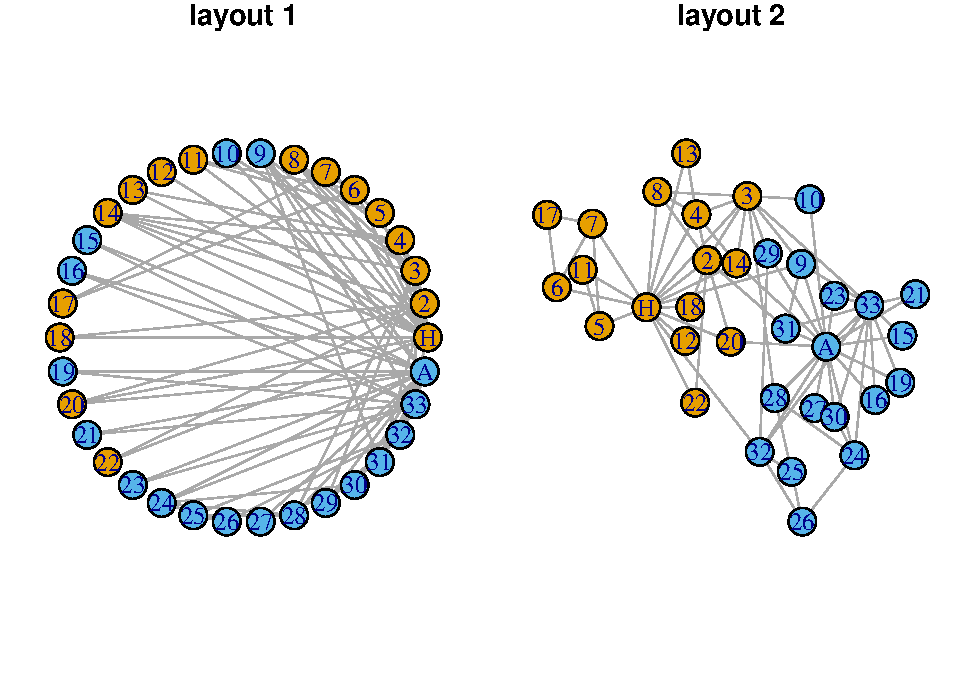
\includegraphics{bookdown-demo_files/figure-latex/unnamed-chunk-165-1.pdf} 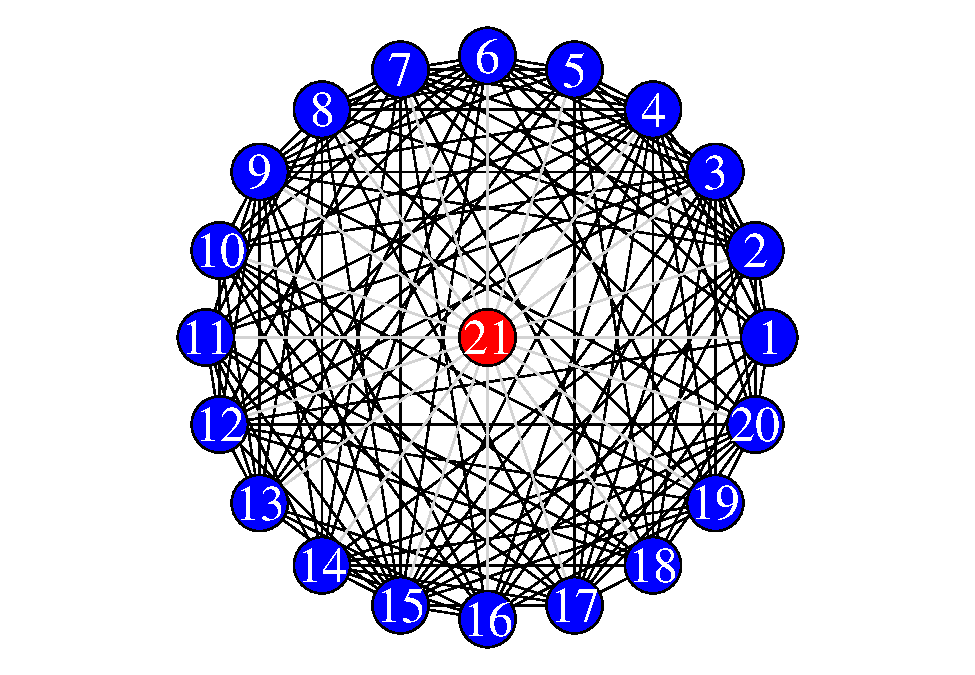
\includegraphics{bookdown-demo_files/figure-latex/unnamed-chunk-165-2.pdf}

Let's compute the ENS and local C for the ego node in the smaller neighborhood (using both the corresponding functions and the mathematical equations):

\begin{Shaded}
\begin{Highlighting}[]
\CommentTok{\# the ego node is node 1 in the g\_small network }

\FunctionTok{transitivity}\NormalTok{(g\_small, }\AttributeTok{type =} \StringTok{\textquotesingle{}local\textquotesingle{}}\NormalTok{, }\AttributeTok{vids =} \DecValTok{1}\NormalTok{)}
\end{Highlighting}
\end{Shaded}

\begin{verbatim}
## [1] 0.7
\end{verbatim}

\begin{Shaded}
\begin{Highlighting}[]
\CommentTok{\# number of ties / number of possible ties among neighbors }
\CommentTok{\# t / (k(k{-}1)/2)}
\DecValTok{7}\SpecialCharTok{/}\NormalTok{(}\DecValTok{5}\SpecialCharTok{*}\NormalTok{(}\DecValTok{5{-}1}\NormalTok{)}\SpecialCharTok{/}\DecValTok{2}\NormalTok{) }
\end{Highlighting}
\end{Shaded}

\begin{verbatim}
## [1] 0.7
\end{verbatim}

\begin{Shaded}
\begin{Highlighting}[]
\FunctionTok{ens}\NormalTok{(g\_small)[}\DecValTok{1}\NormalTok{]}
\end{Highlighting}
\end{Shaded}

\begin{verbatim}
## [1] 2.2
\end{verbatim}

\begin{Shaded}
\begin{Highlighting}[]
\CommentTok{\# k {-} (2t/k)}
\DecValTok{5} \SpecialCharTok{{-}}\NormalTok{ (}\DecValTok{2}\SpecialCharTok{*}\DecValTok{7}\SpecialCharTok{/}\DecValTok{5}\NormalTok{)}
\end{Highlighting}
\end{Shaded}

\begin{verbatim}
## [1] 2.2
\end{verbatim}

Let's also compute the ENS and local C for the ego node in the larger neighborhood (using both the corresponding functions and the mathematical equations):

\begin{Shaded}
\begin{Highlighting}[]
\CommentTok{\# the ego node is node 21 in the g\_large network }

\FunctionTok{transitivity}\NormalTok{(g\_large, }\AttributeTok{type =} \StringTok{\textquotesingle{}local\textquotesingle{}}\NormalTok{, }\AttributeTok{vids =} \DecValTok{21}\NormalTok{)}
\end{Highlighting}
\end{Shaded}

\begin{verbatim}
##  21 
## 0.7
\end{verbatim}

\begin{Shaded}
\begin{Highlighting}[]
\CommentTok{\# number of ties / number of possible ties among neighbors }
\CommentTok{\# t / (k(k{-}1)/2)}
\DecValTok{133}\SpecialCharTok{/}\NormalTok{(}\DecValTok{20}\SpecialCharTok{*}\NormalTok{(}\DecValTok{20{-}1}\NormalTok{)}\SpecialCharTok{/}\DecValTok{2}\NormalTok{) }
\end{Highlighting}
\end{Shaded}

\begin{verbatim}
## [1] 0.7
\end{verbatim}

\begin{Shaded}
\begin{Highlighting}[]
\FunctionTok{ens}\NormalTok{(g\_large)[}\DecValTok{21}\NormalTok{]}
\end{Highlighting}
\end{Shaded}

\begin{verbatim}
##  21 
## 6.7
\end{verbatim}

\begin{Shaded}
\begin{Highlighting}[]
\CommentTok{\# k {-} (2t/k)}
\DecValTok{20} \SpecialCharTok{{-}}\NormalTok{ (}\DecValTok{2}\SpecialCharTok{*}\DecValTok{133}\SpecialCharTok{/}\DecValTok{20}\NormalTok{)}
\end{Highlighting}
\end{Shaded}

\begin{verbatim}
## [1] 6.7
\end{verbatim}

What you will notice is that although both nodes have a local \emph{C} of 0.7, indicating that 70\% of all possible connections in their immediate neighborhoods are fulfilled, the two nodes have different effective network sizes. The node from the larger neighborhood has a ENS of 6.7 whereas the node from the smaller neighborhood has a ENS of 2.2. The difference in ENS reflects the fact that the node from the larger neighborhood has more potential in its ability to fill/exploit structural holes in their network than the node from the smaller neighborhood, due to the former having a larger neighborhood to begin with. This is despite both nodes having the same level of interconnectivity within their neighborhoods.

\subsection{Important note about directed graphs}\label{important-note-about-directed-graphs-1}

The \texttt{ens} function does not work as expected when edges are directed. Negative scores and scores less than 1 could arise from running this function on graphs with directed edges. Hence, please convert directed graphs into undirected graphs before proceeding (see Chapter 5.5, \texttt{as.undirected()} function).

\section{References}\label{references-2}

Burt, R. S. (2004). Structural holes and good ideas. \emph{American Journal of Sociology, 110}(2), 349-399.

Granovetter, M. S. (1973). The strength of weak ties. \emph{American Journal of Sociology, 78}(6), 1360-1380.

Valente, T. W., \& Fujimoto, K. (2010). Bridging: locating critical connectors in a network. \emph{Social Networks, 32}(3), 212-220.

\section{Exercise}\label{exercise-8}

Conduct the following analysis on a social network of your choosing, where the nodes correspond to individual persons. If you do not have a social network, you could conduct the analysis on the \texttt{karate} or \texttt{UKfaculty} networks from the \texttt{igraphdata} library.

\begin{enumerate}
\def\labelenumi{\arabic{enumi}.}
\tightlist
\item
  Identify the individuals with the highest and lowest bridging scores.
\end{enumerate}

\begin{itemize}
\tightlist
\item
  What is the implication of having a high bridging score for this particular network?
\item
  What is the implication of having a low bridging score for this particular network?
\end{itemize}

\begin{enumerate}
\def\labelenumi{\arabic{enumi}.}
\setcounter{enumi}{1}
\tightlist
\item
  Identify the individuals with the highest and lowest effective network sizes.
\end{enumerate}

\begin{itemize}
\tightlist
\item
  What is the implication of having a high effective network size for this particular network?
\item
  What is the implication of having a low effective network size for this particular network?
\end{itemize}

\chapter{\texorpdfstring{Chapter 13: \texttt{bootnet} package}{Chapter 13: bootnet package}}\label{ch13}

Psychometrics is the science of psychological measurement. It attempts to measure psychological constructs that are not usually directly observable. The core question in psychometrics is how to relate observable information (questionnaire responses, behaviors, test performance) to theoretical psychological constructs.

The underlying assumption is that the relationship between observables and psychological constructs is that of \emph{common cause}. In other words, there is a hypothesized latent variable (representing the unobservable construct; e.g., intelligence) that causes or leads to the behaviors and responses that are observed (e.g., scores on Raven's Progressive Matrices).

In recent years, a new area known as \textbf{network psychometrics} has developed and gained substantial attention among psychometricians. Instead of trying to uncover a latent variable from observable data, network psychometrics focuses on analyzing the patterns of covariances among observable data as a network representation. This enables researchers to leverage on the network science framework in order to quantify their structural properties.

For instance, Borsboom and Cramer (2013) argue that the complexity of psychopathology demands more sophisticated models that acknowledge its complexity. Traditional psychometric methods that assume a latent variable implicitly assume that clinical symptoms are caused by the disorder itself, but the evidence suggests that symptoms of mental disorders have reliable patterns of covariance that cannot be easily reduced to a single cause or latent variable. Instead of treating mental disorders as a ``disease'' that can be solved by finding the underlying cause(s) (i.e., the ``disease'' model in western medicine), psychometic network models view mental disorders as interactive systems of symptoms with reinforcing negative feedback loops and causal relationships.

\section{Chapter outline}\label{chapter-outline}

Throughout this book we have seen various examples of behavioral networks, and learned about the importance of clearly defining what the nodes and edges are representing. What are the nodes and edges of a psychometric network?

\begin{itemize}
\tightlist
\item
  Nodes: observed variables. In the example that we will work through, these would be the items on the survey that correspond to symptoms associated with post-traumatic stress disorder (PTSD).
\item
  Edges: strength of association between the observed variables. For instance, the strength of the correlation of two symptoms in the PTSD symptom list. This information has to be estimated from the data itself.
\end{itemize}

In the rest of this chapter we will work through a concrete example to show you how to convert data from a survey to a network representation that you can analyze using the functions you've learned about earlier. Thereafter you should be able to apply the same steps to your own data to get the corresponding psychometric network.

\section{\texorpdfstring{Installation of \texttt{bootnet}}{Installation of bootnet}}\label{installation-of-bootnet}

We need to first install the \texttt{bootnet} R library.

\begin{Shaded}
\begin{Highlighting}[]
\FunctionTok{install.packages}\NormalTok{(}\StringTok{\textquotesingle{}bootnet\textquotesingle{}}\NormalTok{)}
\end{Highlighting}
\end{Shaded}

\subsection{\texorpdfstring{\texttt{qgraph} vs.~\texttt{igraph}}{qgraph vs.~igraph}}\label{qgraph-vs.-igraph}

It is important to keep in mind that that network objects created by the \texttt{bootnet} R package are \emph{not} \texttt{igraph} objects; instead, they are \texttt{qgraph} objects, a different class of data objects specially created for \texttt{bootnet} and other packages for psychometric network analysis. In order for you to use the code provided in this book, we will need to first extract the adjacency matrix representation of this object and convert it to an \texttt{igraph} network object. I will show you how to do this later in the chapter.

\section{Dataset}\label{dataset}

The dataset that we will use in this chapter comes from 359 women who were enrolled in a community substance program and met the criteria for either PTSD or sub-threshold PTSD, based on the DSM-IV. This data was obtained from Hien et al.~(2009) and adapted slightly for teaching purposes.

They completed the PTSD Symptom Scale-Self Report (PSS-SR; Foa et al., 1993) by rating the frequency at which they experienced each of symptoms on the following scale: 1 (not at all), 2 (once a week), 3 (2 - 4 times a week), 4 (5 or more times a week).

Foa, E. B., Riggs, D. S., Dancu, C. V., \& Rothbaum, B. O. (1993). Reliability and validity of a brief instrument for assessing post‐traumatic stress disorder. Journal of Traumatic Stress, 6(4), 459-473.

Hien DA, Wells EA, Jiang H, Suarez-Morales L, Campbell AN, Cohen LR, Zhang Y, et al.~Multisite randomized trial of behavioral interventions for women with co-occurring ptsd and substance use disorders. Journal of Consulting and Clinical Psychology. 2009;77(4):607--619. doi: 10.1037/a0016227

As we can see below, there are 17 items in the PSS-SR, corresponding to the columns of the data frame, and 359 responses corresponding to the rows of the data frame. The responses are ordinal and range from 1 to 5.

\begin{Shaded}
\begin{Highlighting}[]
\FunctionTok{load}\NormalTok{(}\StringTok{\textquotesingle{}data/ptsd\_freq.RData\textquotesingle{}}\NormalTok{) }\CommentTok{\# load pre{-}processed data }

\NormalTok{qs\_freq\_wide[}\DecValTok{1}\SpecialCharTok{:}\DecValTok{3}\NormalTok{,}\DecValTok{1}\SpecialCharTok{:}\DecValTok{5}\NormalTok{] }\CommentTok{\# each row = 1 subject, each column = 1 item }
\end{Highlighting}
\end{Shaded}

\begin{verbatim}
## # A tibble: 3 x 5
##   `AVOID REMINDERS OF THE TRAUMA` `BAD DREAMS ABOUT THE TRAUMA` `BEING JUMPY OR EASILY STARTLED` `BEING OVER ALERT` `DISTANT OR CUT OFF FROM PEOPLE`
##                             <dbl>                         <dbl>                            <dbl>              <dbl>                            <dbl>
## 1                               4                             1                                4                  4                                1
## 2                               1                             3                                2                  3                                1
## 3                               4                             2                                1                  2                                2
\end{verbatim}

\begin{Shaded}
\begin{Highlighting}[]
\FunctionTok{colnames}\NormalTok{(qs\_freq\_wide) }\CommentTok{\# list of items }
\end{Highlighting}
\end{Shaded}

\begin{verbatim}
##  [1] "AVOID REMINDERS OF THE TRAUMA"  "BAD DREAMS ABOUT THE TRAUMA"    "BEING JUMPY OR EASILY STARTLED" "BEING OVER ALERT"               "DISTANT OR CUT OFF FROM PEOPLE" "FEELING EMOTIONALLY NUMB"      
##  [7] "FEELING IRRITABLE"              "FEELING PLANS WONT COME TRUE"   "HAVING TROUBLE CONCENTRATING"   "HAVING TROUBLE SLEEPING"        "LESS INTEREST IN ACTIVITIES"    "NOT ABLE TO REMEMBER"          
## [13] "NOT THINKING ABOUT TRAUMA"      "PHYSICAL REACTIONS"             "RELIVING THE TRAUMA"            "UPSET WHEN REMINDED OF TRAUMA"  "UPSETTING THOUGHTS OR IMAGES"
\end{verbatim}

\section{Estimate a partial correlation network}\label{estimate-a-partial-correlation-network}

To represent the associations across the 17 items in our dataset, we will estimate a \emph{partial correlation} network. The partial correlation depicts the strength of association of 2 variables after conditioning on other variables.

We make use of the \texttt{estimateNetwork} function from bootnet to help us do this. To estimate a partial correlation network, we need to specify an additional argument, \texttt{default\ =\ "pcor"}.

\begin{Shaded}
\begin{Highlighting}[]
\FunctionTok{library}\NormalTok{(bootnet)}
\end{Highlighting}
\end{Shaded}

\begin{verbatim}
## This is bootnet 1.6
\end{verbatim}

\begin{verbatim}
## For questions and issues, please see github.com/SachaEpskamp/bootnet.
\end{verbatim}

\begin{Shaded}
\begin{Highlighting}[]
\NormalTok{ptsd\_network }\OtherTok{\textless{}{-}} \FunctionTok{estimateNetwork}\NormalTok{(qs\_freq\_wide, }\AttributeTok{default =} \StringTok{"pcor"}\NormalTok{) }
\end{Highlighting}
\end{Shaded}

\begin{verbatim}
## Estimating Network. Using package::function:
##   - qgraph::qgraph(..., graph = 'pcor') for network computation
##   - psych::corr.p for significance thresholding
\end{verbatim}

\begin{Shaded}
\begin{Highlighting}[]
\CommentTok{\# pcor = partial correlation network}

\FunctionTok{summary}\NormalTok{(ptsd\_network) }\CommentTok{\# how many nodes and edges does this network have?}
\end{Highlighting}
\end{Shaded}

\begin{verbatim}
## 
## === Estimated network ===
## Number of nodes: 17 
## Number of non-zero edges: 136 / 136 
## Mean weight: 0.05363509 
## Network stored in object$graph 
##  
## Default set used: pcor 
##  
## Use plot(object) to plot estimated network 
## Use bootnet(object) to bootstrap edge weights and centrality indices 
## 
## Relevant references:
## 
##      Epskamp, S., Borsboom, D., & Fried, E. I. (2016). Estimating psychological networks and their accuracy: a tutorial paper. arXiv preprint, arXiv:1604.08462.
\end{verbatim}

First, notice, that the \texttt{summary} function gives us a very different output than what we are used to. This is because \texttt{ptsd\_network} is a \texttt{qgraph} object, not an \texttt{igraph} object. That said, the output is quite straightforward and you should be able to tell that there are 17 nodes and 136/136 non-zero edges.

Before proceeding, note that there are several different methods to estimate a network from psychometric data (type in \texttt{?estimateNetwork} into the console to see all of the different estimator methods that \texttt{bootnet} can use). For demonstration purposes, I have shown you just one of those approaches (i.e., partial correlation). In practice, which method you decide on depends on the properties of your data (i.e, is it categorical, continuous, normally distributed?) and how conservative you want your model to be. See ``Additional resources''.

\subsection{Thresholding}\label{thresholding}

\texttt{ptsd\_network} contains 17 nodes and 136/136 non-zero edges. Notice that the number 136 corresponds to the maximum number of edges possible in a network of 17 nodes (test this for your yourself by calculating the number of possible combinations of 2 from 17 options). The presence of 136 non-zero edges indicates that this is in fact a fully connected graph.

A fully connected network is a rather meaningless representation to work with as there will be little to no variance in the node-level measures. Because many of these correlations depict very weak relationships, we can remove such non-significant correlations by including the argument \texttt{threshold\ =\ \textquotesingle{}sig\textquotesingle{}}.

\begin{Shaded}
\begin{Highlighting}[]
\NormalTok{ptsd\_network }\OtherTok{\textless{}{-}} \FunctionTok{estimateNetwork}\NormalTok{(qs\_freq\_wide, }\AttributeTok{default =} \StringTok{"pcor"}\NormalTok{, }
                                \AttributeTok{threshold =} \StringTok{\textquotesingle{}sig\textquotesingle{}}\NormalTok{) }
\end{Highlighting}
\end{Shaded}

\begin{verbatim}
## Estimating Network. Using package::function:
##   - qgraph::qgraph(..., graph = 'pcor') for network computation
##   - psych::corr.p for significance thresholding
\end{verbatim}

\begin{Shaded}
\begin{Highlighting}[]
\CommentTok{\# pcor = partial correlation network, only retain significant edges }

\FunctionTok{summary}\NormalTok{(ptsd\_network) }\CommentTok{\# how many nodes and edges does this network have?}
\end{Highlighting}
\end{Shaded}

\begin{verbatim}
## 
## === Estimated network ===
## Number of nodes: 17 
## Number of non-zero edges: 31 / 136 
## Mean weight: 0.03630966 
## Network stored in object$graph 
##  
## Default set used: pcor 
##  
## Use plot(object) to plot estimated network 
## Use bootnet(object) to bootstrap edge weights and centrality indices 
## 
## Relevant references:
## 
##      Epskamp, S., Borsboom, D., & Fried, E. I. (2016). Estimating psychological networks and their accuracy: a tutorial paper. arXiv preprint, arXiv:1604.08462.
\end{verbatim}

After including statistical significance as a threshold to remove edges depicting weak correlations, \texttt{ptsd\_network} contains 17 nodes and 31 edges.

\subsection{Absolutizing}\label{absolutizing}

We can view the adjacency matrix of the network from running the following:

\begin{Shaded}
\begin{Highlighting}[]
\NormalTok{ptsd\_network}\SpecialCharTok{$}\NormalTok{graph}
\end{Highlighting}
\end{Shaded}

\begin{verbatim}
##            AROTT      BDATT      BJOES       BOA    DOCOFP       FEN       FEI     FPWCT        HTC       HTS      LIIA      NATR      NTAT       PHR       RTT      UWROT      UTOI
## AROTT  0.0000000  0.0000000  0.0000000 0.1555554 0.0000000 0.0000000 0.0000000 0.0000000  0.0000000 0.0000000 0.0000000 0.0000000 0.1515577 0.1746399 0.0000000  0.0000000 0.0000000
## BDATT  0.0000000  0.0000000  0.0000000 0.0000000 0.0000000 0.0000000 0.0000000 0.0000000 -0.1221041 0.0000000 0.0000000 0.0000000 0.0000000 0.1089284 0.0000000  0.1461690 0.1710409
## BJOES  0.0000000  0.0000000  0.0000000 0.4075190 0.0000000 0.0000000 0.0000000 0.0000000  0.0000000 0.0000000 0.1129132 0.0000000 0.1204094 0.1692879 0.0000000 -0.1109757 0.0000000
## BOA    0.1555554  0.0000000  0.4075190 0.0000000 0.0000000 0.1423142 0.0000000 0.0000000  0.0000000 0.0000000 0.0000000 0.0000000 0.0000000 0.0000000 0.0000000  0.0000000 0.0000000
## DOCOFP 0.0000000  0.0000000  0.0000000 0.0000000 0.0000000 0.2357181 0.1334469 0.0000000  0.0000000 0.0000000 0.3509726 0.0000000 0.0000000 0.0000000 0.0000000  0.0000000 0.0000000
## FEN    0.0000000  0.0000000  0.0000000 0.1423142 0.2357181 0.0000000 0.1410481 0.1474119  0.0000000 0.0000000 0.0000000 0.0000000 0.0000000 0.0000000 0.0000000  0.0000000 0.0000000
## FEI    0.0000000  0.0000000  0.0000000 0.0000000 0.1334469 0.1410481 0.0000000 0.1214582  0.1793871 0.0000000 0.0000000 0.0000000 0.0000000 0.0000000 0.0000000  0.0000000 0.0000000
## FPWCT  0.0000000  0.0000000  0.0000000 0.0000000 0.0000000 0.1474119 0.1214582 0.0000000  0.0000000 0.0000000 0.2044012 0.0000000 0.0000000 0.0000000 0.0000000  0.0000000 0.0000000
## HTC    0.0000000 -0.1221041  0.0000000 0.0000000 0.0000000 0.0000000 0.1793871 0.0000000  0.0000000 0.1332300 0.0000000 0.0000000 0.0000000 0.0000000 0.0000000  0.0000000 0.0000000
## HTS    0.0000000  0.0000000  0.0000000 0.0000000 0.0000000 0.0000000 0.0000000 0.0000000  0.1332300 0.0000000 0.0000000 0.0000000 0.0000000 0.0000000 0.0000000  0.0000000 0.1351728
## LIIA   0.0000000  0.0000000  0.1129132 0.0000000 0.3509726 0.0000000 0.0000000 0.2044012  0.0000000 0.0000000 0.0000000 0.0000000 0.0000000 0.0000000 0.1093724  0.0000000 0.0000000
## NATR   0.0000000  0.0000000  0.0000000 0.0000000 0.0000000 0.0000000 0.0000000 0.0000000  0.0000000 0.0000000 0.0000000 0.0000000 0.1711055 0.0000000 0.1487162  0.1546641 0.0000000
## NTAT   0.1515577  0.0000000  0.1204094 0.0000000 0.0000000 0.0000000 0.0000000 0.0000000  0.0000000 0.0000000 0.0000000 0.1711055 0.0000000 0.0000000 0.0000000  0.1169038 0.0000000
## PHR    0.1746399  0.1089284  0.1692879 0.0000000 0.0000000 0.0000000 0.0000000 0.0000000  0.0000000 0.0000000 0.0000000 0.0000000 0.0000000 0.0000000 0.1811024  0.0000000 0.0000000
## RTT    0.0000000  0.0000000  0.0000000 0.0000000 0.0000000 0.0000000 0.0000000 0.0000000  0.0000000 0.0000000 0.1093724 0.1487162 0.0000000 0.1811024 0.0000000  0.0000000 0.1970405
## UWROT  0.0000000  0.1461690 -0.1109757 0.0000000 0.0000000 0.0000000 0.0000000 0.0000000  0.0000000 0.0000000 0.0000000 0.1546641 0.1169038 0.0000000 0.0000000  0.0000000 0.4497070
## UTOI   0.0000000  0.1710409  0.0000000 0.0000000 0.0000000 0.0000000 0.0000000 0.0000000  0.0000000 0.1351728 0.0000000 0.0000000 0.0000000 0.0000000 0.1970405  0.4497070 0.0000000
\end{verbatim}

You may notice from the adjacency matrix that some partial correlations are negative. For instance, the correlation between HTC and BDATT is -0.1221041. However, when edge weights are negative, certain network measures cannot be computed and so we need to convert them to a positive value (but maintain the magnitude of the effect). Edges that depict a ``positive'' or ``negative'' meaning are associated with the theory of \href{https://en.wikipedia.org/wiki/Signed_network}{signed networks}, which are beyond the scope of this book. Interested readers can refer to the \href{https://www.r-bloggers.com/2020/01/a-package-for-analysing-signed-networks/}{\texttt{signnet} R package} for further information about how to analyze signed networks.

The code below shows you how to absolutize the matrix and assigns the output as a new data object \texttt{my\_adj\_mat}.

\begin{Shaded}
\begin{Highlighting}[]
\CommentTok{\# make all edge weights positive }
\NormalTok{my\_adj\_mat }\OtherTok{\textless{}{-}} \FunctionTok{abs}\NormalTok{(ptsd\_network}\SpecialCharTok{$}\NormalTok{graph)}

\NormalTok{my\_adj\_mat[}\DecValTok{1}\SpecialCharTok{:}\DecValTok{10}\NormalTok{,}\DecValTok{1}\SpecialCharTok{:}\DecValTok{7}\NormalTok{]}
\end{Highlighting}
\end{Shaded}

\begin{verbatim}
##            AROTT     BDATT    BJOES       BOA    DOCOFP       FEN       FEI
## AROTT  0.0000000 0.0000000 0.000000 0.1555554 0.0000000 0.0000000 0.0000000
## BDATT  0.0000000 0.0000000 0.000000 0.0000000 0.0000000 0.0000000 0.0000000
## BJOES  0.0000000 0.0000000 0.000000 0.4075190 0.0000000 0.0000000 0.0000000
## BOA    0.1555554 0.0000000 0.407519 0.0000000 0.0000000 0.1423142 0.0000000
## DOCOFP 0.0000000 0.0000000 0.000000 0.0000000 0.0000000 0.2357181 0.1334469
## FEN    0.0000000 0.0000000 0.000000 0.1423142 0.2357181 0.0000000 0.1410481
## FEI    0.0000000 0.0000000 0.000000 0.0000000 0.1334469 0.1410481 0.0000000
## FPWCT  0.0000000 0.0000000 0.000000 0.0000000 0.0000000 0.1474119 0.1214582
## HTC    0.0000000 0.1221041 0.000000 0.0000000 0.0000000 0.0000000 0.1793871
## HTS    0.0000000 0.0000000 0.000000 0.0000000 0.0000000 0.0000000 0.0000000
\end{verbatim}

\subsection{Conversion to igraph}\label{conversion-to-igraph}

In the final step, we need to convert the matrix object into an \texttt{igraph} network, using a function that should be familiar to you by now! (see Chapter 2/3).

\begin{Shaded}
\begin{Highlighting}[]
\FunctionTok{library}\NormalTok{(igraph) }\CommentTok{\# load the package}

\CommentTok{\# why we should use this particular function? }
\NormalTok{ptsd\_network\_igraph }\OtherTok{\textless{}{-}} \FunctionTok{graph\_from\_adjacency\_matrix}\NormalTok{(my\_adj\_mat, }
                                                   \AttributeTok{mode =} \StringTok{\textquotesingle{}undirected\textquotesingle{}}\NormalTok{, }
                                                   \AttributeTok{weighted =} \ConstantTok{TRUE}\NormalTok{)}

\FunctionTok{summary}\NormalTok{(ptsd\_network\_igraph)}
\end{Highlighting}
\end{Shaded}

\begin{verbatim}
## IGRAPH d4fe76d UNW- 17 31 -- 
## + attr: name (v/c), weight (e/n)
\end{verbatim}

We can easily see that the network contains 17 nodes and 31 edges, and is an undirected and weighted graph. The weights correspond to the strength of the partial correlation between those two items, and only significant correlations were retained as edges. The edges are undirected because direction of causality cannot be inferred from the correlations.

Thereafter, we can easily compute various network measures for the network.

\begin{Shaded}
\begin{Highlighting}[]
\CommentTok{\# degree of nodes}
\FunctionTok{degree}\NormalTok{(ptsd\_network\_igraph)}
\end{Highlighting}
\end{Shaded}

\begin{verbatim}
##  AROTT  BDATT  BJOES    BOA DOCOFP    FEN    FEI  FPWCT    HTC    HTS   LIIA   NATR   NTAT    PHR    RTT  UWROT   UTOI 
##      3      4      5      3      3      4      4      3      3      2      4      3      4      4      4      5      4
\end{verbatim}

\begin{Shaded}
\begin{Highlighting}[]
\CommentTok{\# global clustering coefficient }
\FunctionTok{transitivity}\NormalTok{(ptsd\_network\_igraph, }\AttributeTok{type =} \StringTok{\textquotesingle{}global\textquotesingle{}}\NormalTok{)}
\end{Highlighting}
\end{Shaded}

\begin{verbatim}
## [1] 0.1724138
\end{verbatim}

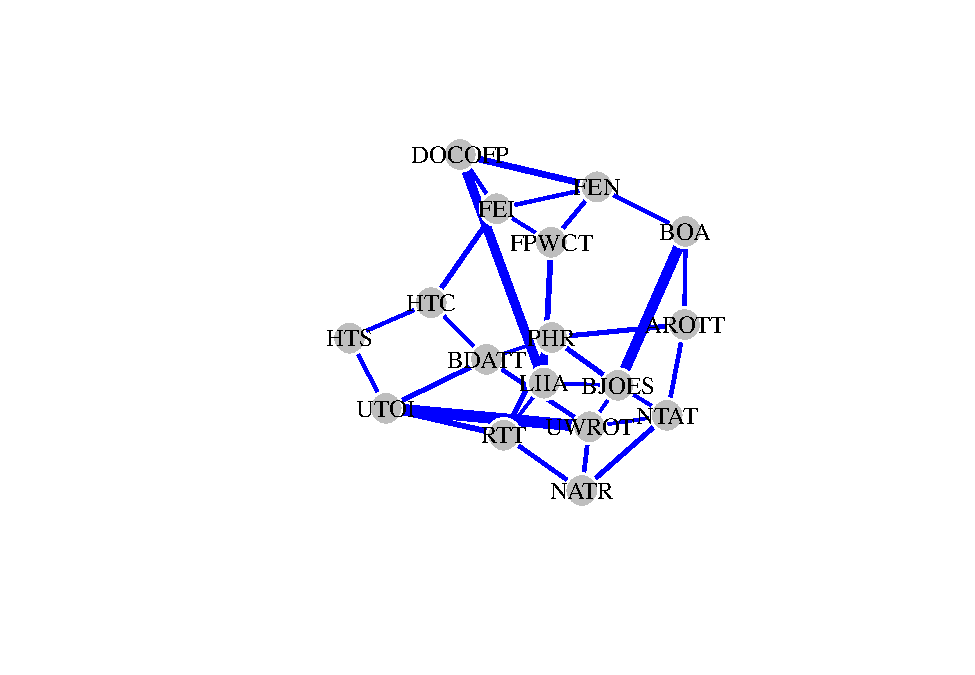
\includegraphics{bookdown-demo_files/figure-latex/test-1.pdf}

\section{Sample sizes}\label{sample-sizes}

A common pitfall when trying to use \texttt{bootnet} to estimate a network occurs when sample sizes are simply too small in order to robustly estimate the covariance structure (\texttt{bootnet} throws an error or returns a network with 0 edges). In such cases, the best solution is to collect more data or find larger datasets. If one insists on sticking with the low-quality dataset, it is always possible to estimate a correlation matrix through other packages and conduct your own thresholding, since it is non-trivial to convert any numeric (adjacency) matrix into a network. But this is not recommended practice.

\section{Additional resources}\label{additional-resources}

Epskamp, S., Borsboom, D., \& Fried, E. I. (2018). Estimating psychological networks and their accuracy: A tutorial paper. Behavior Research Methods, 50(1), 195-212.

Snijders, T. A., \& Borgatti, S. P. (1999). Non-parametric standard errors and tests for network statistics. Connections, 22(2), 161-170.

Isvoranu, A.-M., Epskamp, S., Waldorp, L., \& Borsboom, D. (Eds.). (2022). Network Psychometrics with R: A Guide for Behavioral and Social Scientists (1st ed.). Routledge. \url{https://doi.org/10.4324/9781003111238}

\chapter{\texorpdfstring{Chapter 14: Network visualization in \texttt{igraph}}{Chapter 14: Network visualization in igraph}}\label{ch14}

This chapter aims to introduce you the basics of network visualization. Note that for a very large network (\textgreater{} 100 nodes) it becomes very difficult to create good visualizations using basic \texttt{igraph} plotting functions. You may need to venture to other R packages (see Chapter 15 - under development). A nice open-source software for creating great network visualizations is \href{https://gephi.org/}{Gephi}.

\section{Set up}\label{set-up-3}

We will use the \texttt{karate} network from Chapter 5, which contains various node and edge attributes.

\begin{Shaded}
\begin{Highlighting}[]
\FunctionTok{library}\NormalTok{(igraph)}
\FunctionTok{library}\NormalTok{(igraphdata)}
\FunctionTok{library}\NormalTok{(tidyverse)}

\FunctionTok{data}\NormalTok{(}\StringTok{\textquotesingle{}karate\textquotesingle{}}\NormalTok{)}

\CommentTok{\# import your node attributes }
\NormalTok{node\_info }\OtherTok{\textless{}{-}} \FunctionTok{read.csv}\NormalTok{(}\StringTok{\textquotesingle{}data/karate\_nodes\_added.csv\textquotesingle{}}\NormalTok{, }\AttributeTok{header =}\NormalTok{ T)}

\CommentTok{\# very important to ensure that node order is identical }
\NormalTok{node\_info }\OtherTok{\textless{}{-}}\NormalTok{ node\_info }\SpecialCharTok{\%\textgreater{}\%} \FunctionTok{arrange}\NormalTok{(}\FunctionTok{factor}\NormalTok{(node, }\AttributeTok{levels =} \FunctionTok{V}\NormalTok{(karate)}\SpecialCharTok{$}\NormalTok{name))}
\end{Highlighting}
\end{Shaded}

\begin{verbatim}
## This graph was created by an old(er) igraph version.
##   Call upgrade_graph() on it to use with the current igraph version
##   For now we convert it on the fly...
\end{verbatim}

\begin{Shaded}
\begin{Highlighting}[]
\FunctionTok{identical}\NormalTok{(}\FunctionTok{V}\NormalTok{(karate)}\SpecialCharTok{$}\NormalTok{name, node\_info}\SpecialCharTok{$}\NormalTok{node) }\CommentTok{\# sanity check that the node name order is identical}
\end{Highlighting}
\end{Shaded}

\begin{verbatim}
## [1] TRUE
\end{verbatim}

\begin{Shaded}
\begin{Highlighting}[]
\CommentTok{\# add the \textquotesingle{}gender\textquotesingle{} attribute}
\NormalTok{karate }\OtherTok{\textless{}{-}} \FunctionTok{set\_vertex\_attr}\NormalTok{(karate, }
                          \AttributeTok{name =} \StringTok{\textquotesingle{}gender\textquotesingle{}}\NormalTok{,}
                          \AttributeTok{value =}\NormalTok{ node\_info}\SpecialCharTok{$}\NormalTok{gender)}

\CommentTok{\# add the \textquotesingle{}belt\textquotesingle{} attribute}
\NormalTok{karate }\OtherTok{\textless{}{-}} \FunctionTok{set\_vertex\_attr}\NormalTok{(karate, }
                          \AttributeTok{name =} \StringTok{\textquotesingle{}belt\textquotesingle{}}\NormalTok{,}
                          \AttributeTok{value =}\NormalTok{ node\_info}\SpecialCharTok{$}\NormalTok{belt)}

\CommentTok{\# add the \textquotesingle{}age\textquotesingle{} attribute }
\NormalTok{karate }\OtherTok{\textless{}{-}} \FunctionTok{set\_vertex\_attr}\NormalTok{(karate, }
                          \AttributeTok{name =} \StringTok{\textquotesingle{}age\textquotesingle{}}\NormalTok{,}
                          \AttributeTok{value =}\NormalTok{ node\_info}\SpecialCharTok{$}\NormalTok{age)}

\CommentTok{\# initialize all edges with the same label }
\FunctionTok{E}\NormalTok{(karate)}\SpecialCharTok{$}\NormalTok{edge\_type }\OtherTok{\textless{}{-}} \StringTok{\textquotesingle{}same\textquotesingle{}} 

\CommentTok{\# re{-}assign those with mixed edges to a new label }
\FunctionTok{E}\NormalTok{(karate)}\SpecialCharTok{$}\NormalTok{edge\_type[}\FunctionTok{E}\NormalTok{(karate)[}\FunctionTok{V}\NormalTok{(karate)[}\FunctionTok{V}\NormalTok{(karate)}\SpecialCharTok{$}\NormalTok{gender }\SpecialCharTok{==} \StringTok{\textquotesingle{}male\textquotesingle{}}\NormalTok{] }\SpecialCharTok{\%{-}{-}\%} \FunctionTok{V}\NormalTok{(karate)[}\FunctionTok{V}\NormalTok{(karate)}\SpecialCharTok{$}\NormalTok{gender }\SpecialCharTok{==} \StringTok{\textquotesingle{}female\textquotesingle{}}\NormalTok{]]] }\OtherTok{\textless{}{-}} \StringTok{\textquotesingle{}different\textquotesingle{}}

\FunctionTok{summary}\NormalTok{(karate) }\CommentTok{\# there should be a new edge type }
\end{Highlighting}
\end{Shaded}

\begin{verbatim}
## IGRAPH 4b458a1 UNW- 34 78 -- Zachary's karate club network
## + attr: name (g/c), Citation (g/c), Author (g/c), Faction (v/n), name (v/c), label (v/c), color (v/n), gender (v/c), belt (v/c), age (v/n), weight (e/n), edge_type (e/c)
\end{verbatim}

\section{Visualizing node attributes}\label{visualizing-node-attributes}

\subsection{Color nodes by their categorical attributes}\label{color-nodes-by-their-categorical-attributes}

\begin{Shaded}
\begin{Highlighting}[]
\CommentTok{\# color nodes by their attributes (categorical)}
\FunctionTok{plot}\NormalTok{(karate, }\AttributeTok{vertex.color =} \FunctionTok{factor}\NormalTok{( }\FunctionTok{V}\NormalTok{(karate)}\SpecialCharTok{$}\NormalTok{gender )) }\CommentTok{\# notice the use of factor() }
\end{Highlighting}
\end{Shaded}

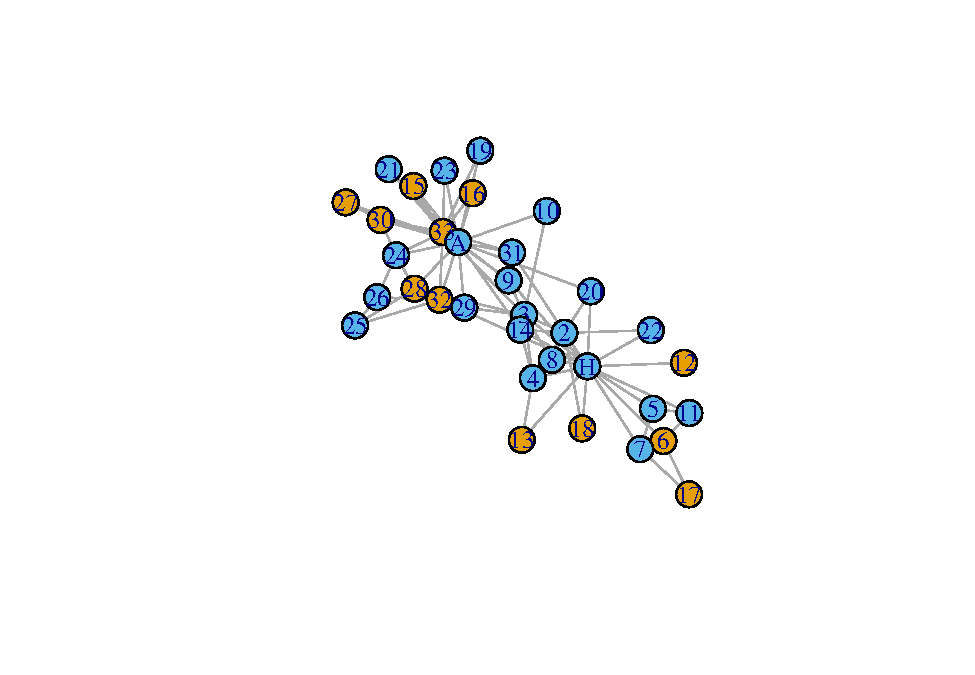
\includegraphics{bookdown-demo_files/figure-latex/unnamed-chunk-177-1.pdf}

\begin{Shaded}
\begin{Highlighting}[]
\CommentTok{\# plot(karate, vertex.color = V(karate)$gender) \# this throws an error }
\end{Highlighting}
\end{Shaded}

If you would like to specify your own colors, you can refer to \href{https://r-charts.com/colors/}{this website} for the names of colors in R and assign them to each category as shown in the following code:

\begin{Shaded}
\begin{Highlighting}[]
\FunctionTok{factor}\NormalTok{( }\FunctionTok{V}\NormalTok{(karate)}\SpecialCharTok{$}\NormalTok{gender ) }\SpecialCharTok{|\textgreater{}} \FunctionTok{levels}\NormalTok{() }\CommentTok{\# order of levels is female male}
\end{Highlighting}
\end{Shaded}

\begin{verbatim}
## [1] "female" "male"
\end{verbatim}

\begin{Shaded}
\begin{Highlighting}[]
\NormalTok{my\_colors }\OtherTok{\textless{}{-}} \FunctionTok{c}\NormalTok{(}\StringTok{\textquotesingle{}firebrick\textquotesingle{}}\NormalTok{, }\StringTok{\textquotesingle{}slateblue\textquotesingle{}}\NormalTok{) }\CommentTok{\# firebrick = female, slateblue = male}

\CommentTok{\# use of square brackets to map the colors onto the labels }
\FunctionTok{plot}\NormalTok{(karate, }\AttributeTok{vertex.color =}\NormalTok{ my\_colors[ }\FunctionTok{factor}\NormalTok{( }\FunctionTok{V}\NormalTok{(karate)}\SpecialCharTok{$}\NormalTok{gender ) ] ,}
     \AttributeTok{vertex.label.color =} \StringTok{\textquotesingle{}white\textquotesingle{}} \CommentTok{\# to make the labels visible}
\NormalTok{     )}
\end{Highlighting}
\end{Shaded}

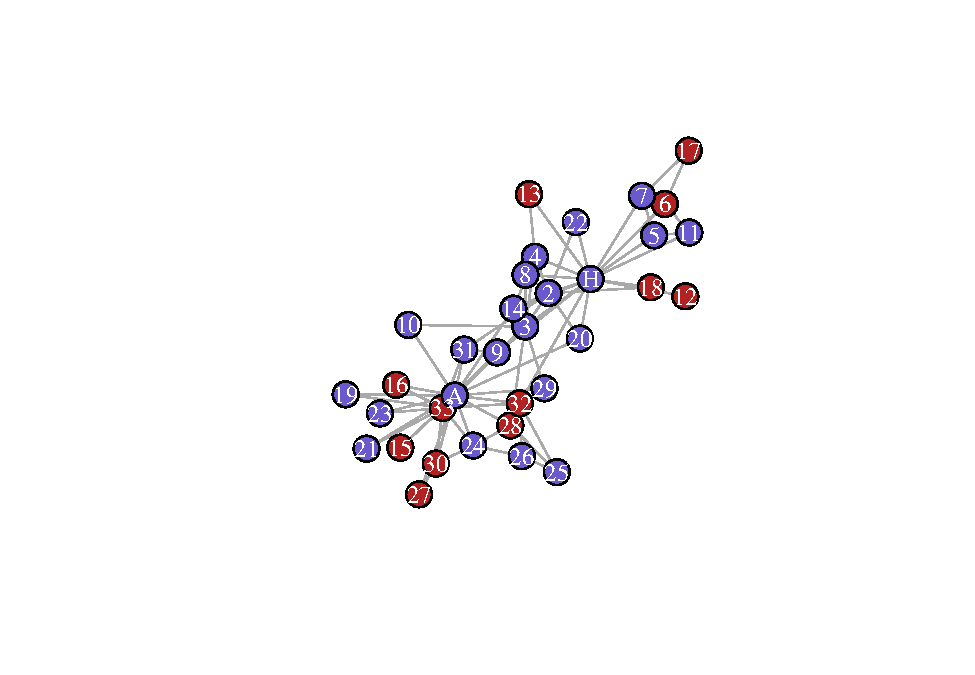
\includegraphics{bookdown-demo_files/figure-latex/unnamed-chunk-178-1.pdf}

Can you try replacing the \texttt{gender} attribute with the \texttt{belt} attribute?

\subsection{Color nodes by their continuous attributes}\label{color-nodes-by-their-continuous-attributes}

\begin{Shaded}
\begin{Highlighting}[]
\CommentTok{\# color nodes by their attributes (continuous) }

\CommentTok{\# a function to generate color gradients from a pre{-}specified palette }
\NormalTok{palf }\OtherTok{\textless{}{-}} \FunctionTok{colorRampPalette}\NormalTok{(}\FunctionTok{c}\NormalTok{(}\StringTok{"red"}\NormalTok{, }\StringTok{"green"}\NormalTok{)) }\CommentTok{\# smaller values = white }

\FunctionTok{plot}\NormalTok{(}\AttributeTok{x=}\DecValTok{10}\SpecialCharTok{:}\DecValTok{1}\NormalTok{, }\AttributeTok{y=}\DecValTok{1}\SpecialCharTok{:}\DecValTok{10}\NormalTok{, }\AttributeTok{pch=}\DecValTok{19}\NormalTok{, }\AttributeTok{cex=}\DecValTok{5}\NormalTok{, }\AttributeTok{col=}\FunctionTok{palf}\NormalTok{(}\DecValTok{10}\NormalTok{))}
\end{Highlighting}
\end{Shaded}

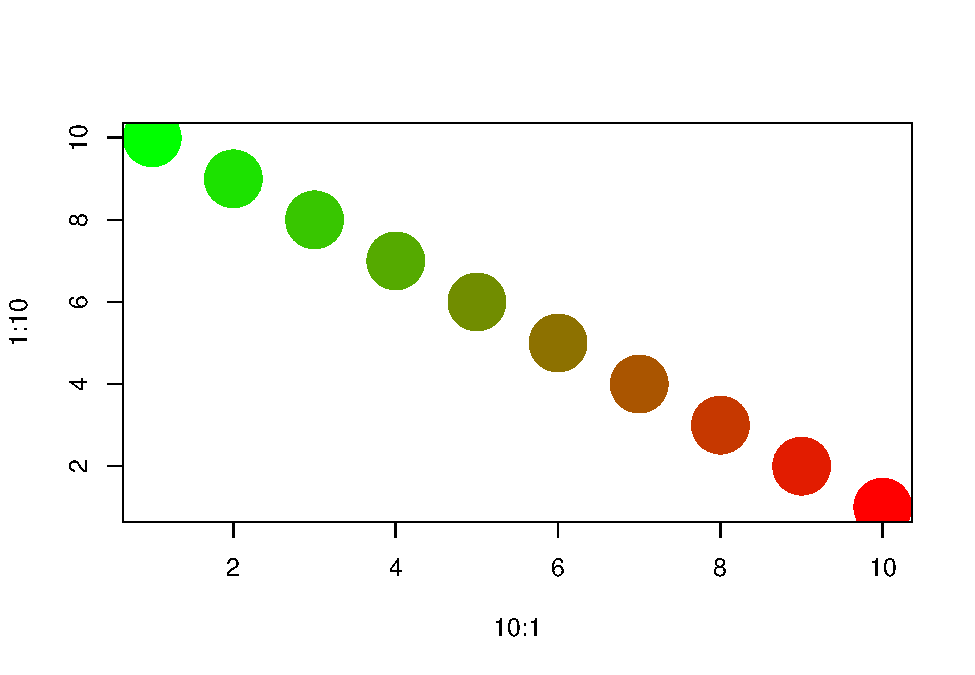
\includegraphics{bookdown-demo_files/figure-latex/unnamed-chunk-179-1.pdf}

\begin{Shaded}
\begin{Highlighting}[]
\FunctionTok{plot}\NormalTok{(karate, }\AttributeTok{vertex.color =} \FunctionTok{palf}\NormalTok{(}\DecValTok{10}\NormalTok{)[}\FunctionTok{cut}\NormalTok{(}\FunctionTok{V}\NormalTok{(karate)}\SpecialCharTok{$}\NormalTok{age, }\DecValTok{10}\NormalTok{)]) }\CommentTok{\# notice the use of cut() }
\end{Highlighting}
\end{Shaded}

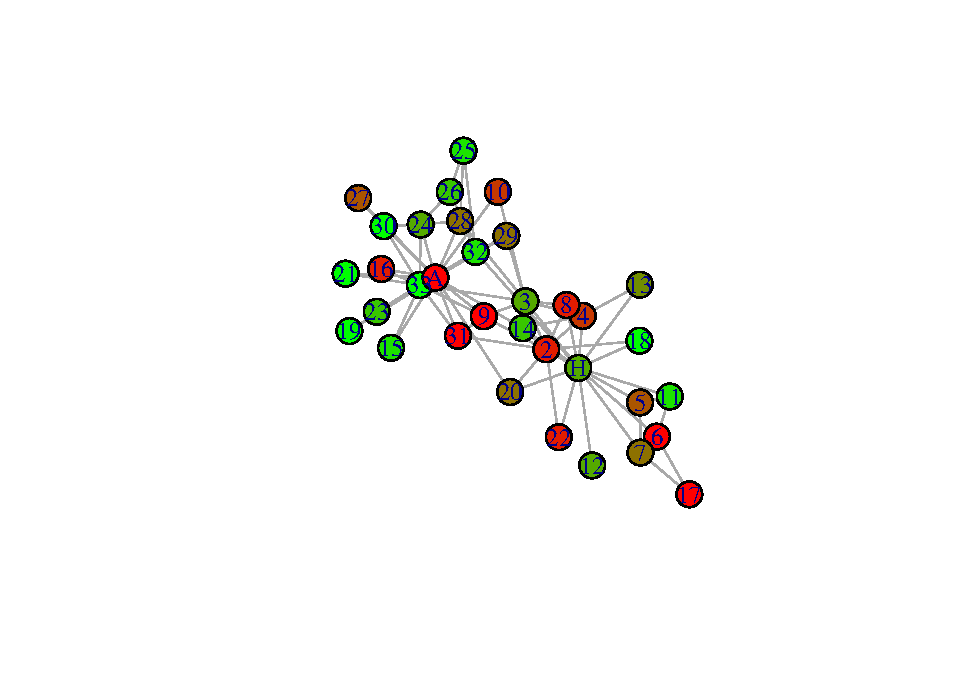
\includegraphics{bookdown-demo_files/figure-latex/unnamed-chunk-179-2.pdf}

\begin{Shaded}
\begin{Highlighting}[]
\CommentTok{\# cut() chops up the age distribution into 10 bins, each bin is assigned to the color gradient based on the order }
\CommentTok{\# the number of bins and color bins must be the same }
\end{Highlighting}
\end{Shaded}

\subsection{Node shapes by their categorical attributes}\label{node-shapes-by-their-categorical-attributes}

\begin{Shaded}
\begin{Highlighting}[]
\CommentTok{\# give categorical attributes different shapes }
\FunctionTok{plot}\NormalTok{(karate, }
     \AttributeTok{vertex.shape =} \FunctionTok{c}\NormalTok{(}\StringTok{\textquotesingle{}circle\textquotesingle{}}\NormalTok{, }\StringTok{\textquotesingle{}square\textquotesingle{}}\NormalTok{)[}\FunctionTok{factor}\NormalTok{(}\FunctionTok{V}\NormalTok{(karate)}\SpecialCharTok{$}\NormalTok{gender)], }\CommentTok{\# notice the use of factor() with gender to subset a vector of pre{-}defined node shapes}
     \AttributeTok{vertex.color =} \StringTok{\textquotesingle{}white\textquotesingle{}}\NormalTok{) }
\end{Highlighting}
\end{Shaded}

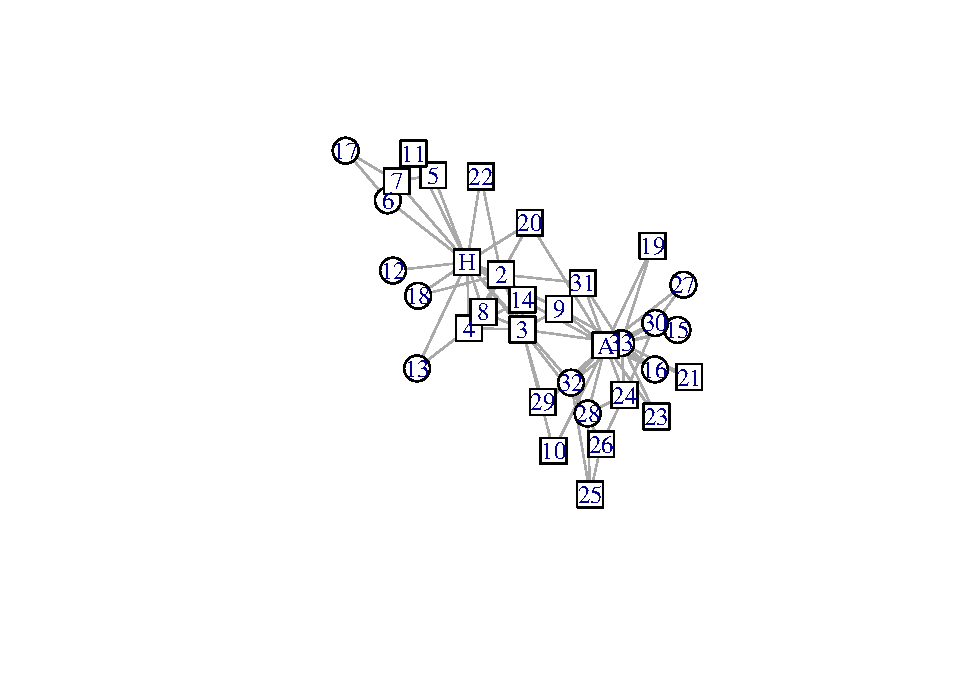
\includegraphics{bookdown-demo_files/figure-latex/unnamed-chunk-180-1.pdf}

\begin{Shaded}
\begin{Highlighting}[]
\FunctionTok{factor}\NormalTok{(}\FunctionTok{V}\NormalTok{(karate)}\SpecialCharTok{$}\NormalTok{gender) }\SpecialCharTok{|\textgreater{}} \FunctionTok{levels}\NormalTok{() }\CommentTok{\# female/circle, male/square}
\end{Highlighting}
\end{Shaded}

\begin{verbatim}
## [1] "female" "male"
\end{verbatim}

\subsection{Node size by their continuous attributes}\label{node-size-by-their-continuous-attributes}

\begin{Shaded}
\begin{Highlighting}[]
\CommentTok{\# give continuous attributes different sizes }

\FunctionTok{plot}\NormalTok{(karate, }\AttributeTok{vertex.size =} \FunctionTok{V}\NormalTok{(karate)}\SpecialCharTok{$}\NormalTok{age) }\CommentTok{\# notice that the sizes are not very well scaled }
\end{Highlighting}
\end{Shaded}

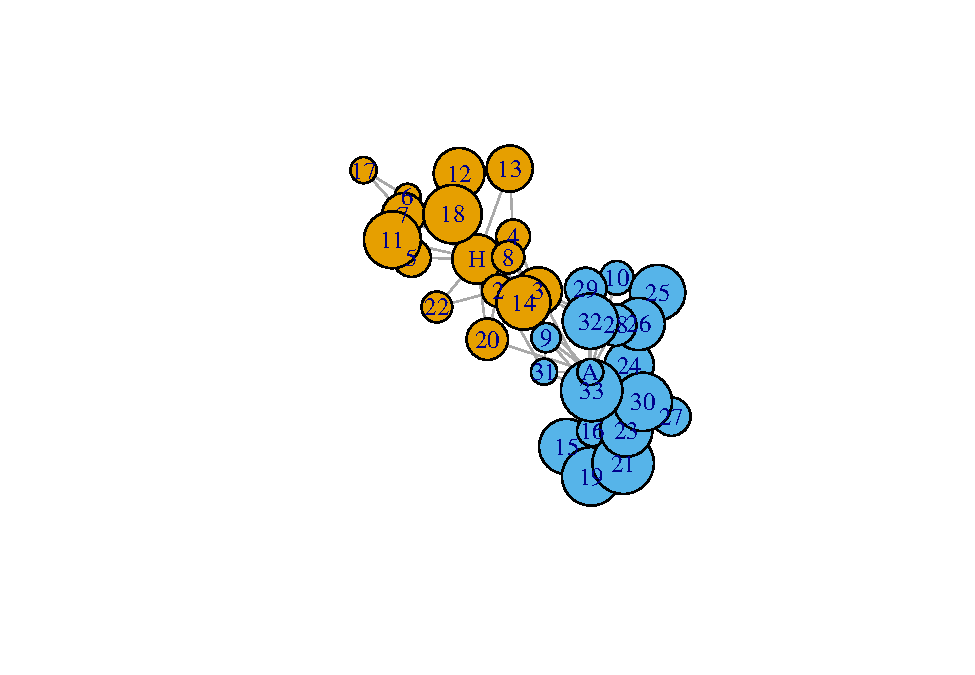
\includegraphics{bookdown-demo_files/figure-latex/unnamed-chunk-181-1.pdf}

\begin{Shaded}
\begin{Highlighting}[]
\FunctionTok{plot}\NormalTok{(karate, }\AttributeTok{vertex.size =} \FloatTok{0.5}\SpecialCharTok{*}\FunctionTok{V}\NormalTok{(karate)}\SpecialCharTok{$}\NormalTok{age) }\CommentTok{\# you will have to play around to find a suitable scale }
\end{Highlighting}
\end{Shaded}

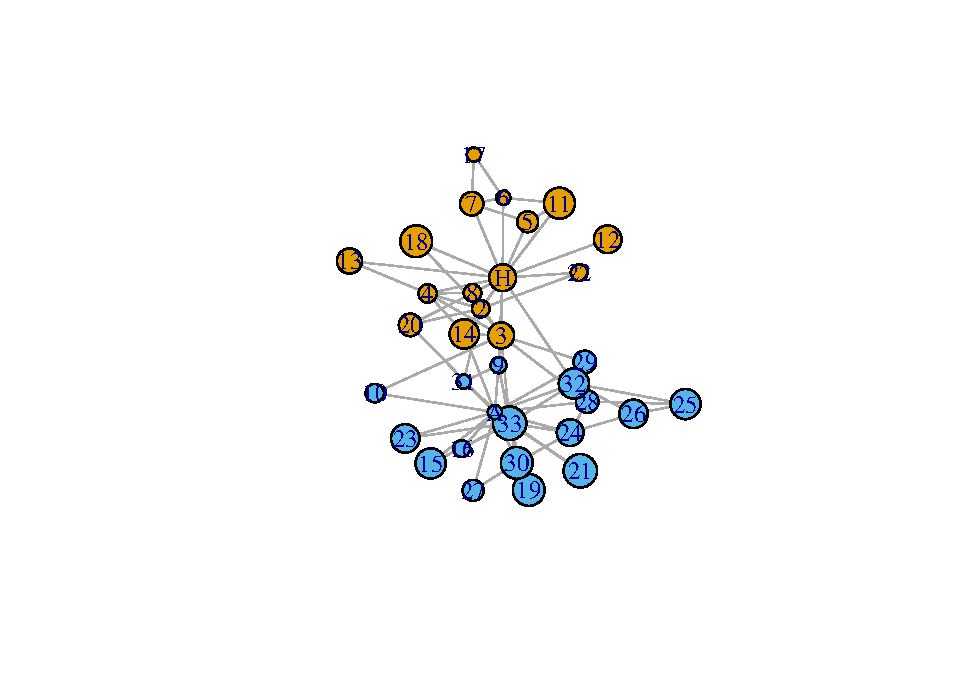
\includegraphics{bookdown-demo_files/figure-latex/unnamed-chunk-181-2.pdf}

\subsection{Example 1: Color nodes by their community membership}\label{example-1-color-nodes-by-their-community-membership}

\begin{Shaded}
\begin{Highlighting}[]
\FunctionTok{set.seed}\NormalTok{(}\DecValTok{1}\NormalTok{)}
\NormalTok{community\_result }\OtherTok{\textless{}{-}} \FunctionTok{cluster\_louvain}\NormalTok{(karate)}

\FunctionTok{V}\NormalTok{(karate)}\SpecialCharTok{$}\NormalTok{community }\OtherTok{\textless{}{-}}\NormalTok{ community\_result}\SpecialCharTok{$}\NormalTok{membership}

\FunctionTok{plot}\NormalTok{(karate, }\AttributeTok{vertex.color =} \FunctionTok{V}\NormalTok{(karate)}\SpecialCharTok{$}\NormalTok{community)}
\end{Highlighting}
\end{Shaded}

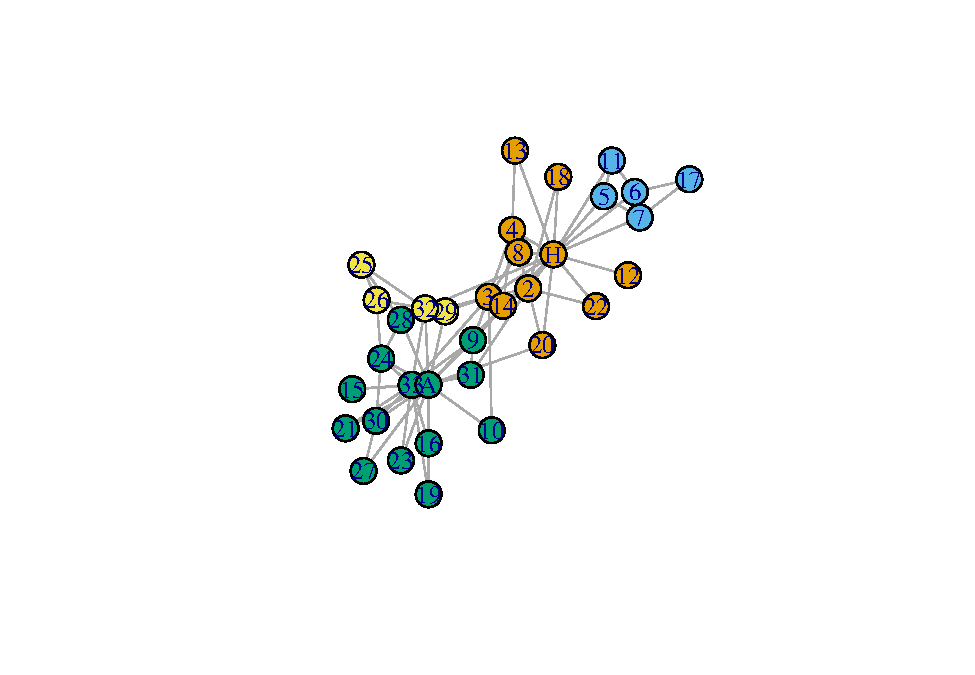
\includegraphics{bookdown-demo_files/figure-latex/unnamed-chunk-182-1.pdf}

\subsection{Example 2: Size nodes by their degree}\label{example-2-size-nodes-by-their-degree}

\begin{Shaded}
\begin{Highlighting}[]
\FunctionTok{plot}\NormalTok{(karate, }\AttributeTok{vertex.size =} \FunctionTok{degree}\NormalTok{(karate), }\AttributeTok{vertex.color =} \StringTok{\textquotesingle{}black\textquotesingle{}}\NormalTok{) }\CommentTok{\# the scaling issue may apply here }
\end{Highlighting}
\end{Shaded}

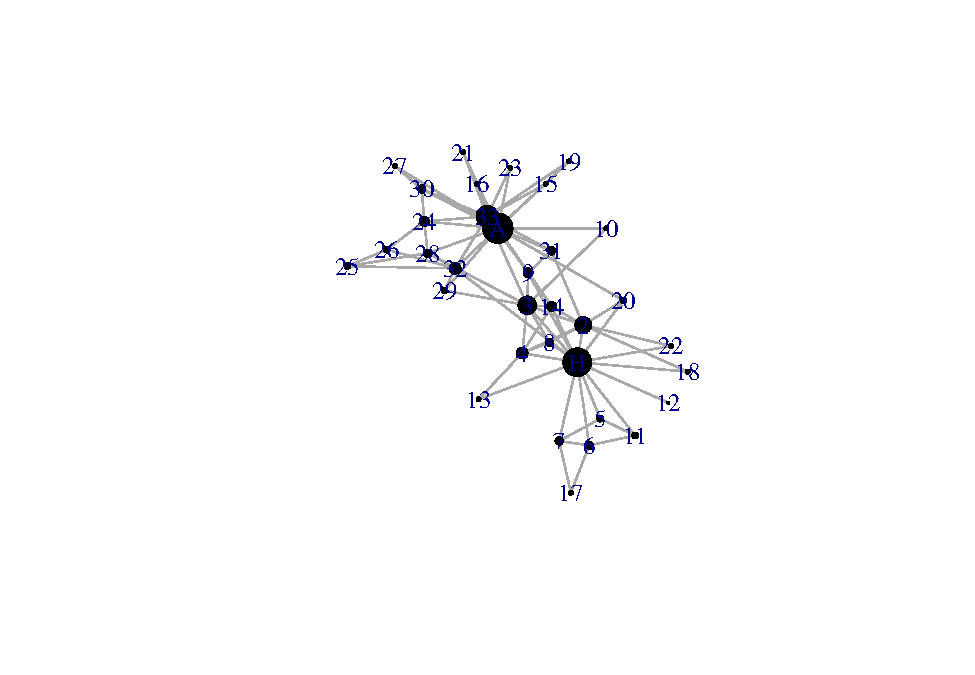
\includegraphics{bookdown-demo_files/figure-latex/unnamed-chunk-183-1.pdf}

\section{Visualizing edge attributes}\label{visualizing-edge-attributes}

\subsection{Color edges by their categorical attributes}\label{color-edges-by-their-categorical-attributes}

\begin{Shaded}
\begin{Highlighting}[]
\FunctionTok{plot}\NormalTok{(karate, }\AttributeTok{vertex.color =} \StringTok{\textquotesingle{}white\textquotesingle{}}\NormalTok{, }\AttributeTok{edge.color =} \FunctionTok{factor}\NormalTok{(}\FunctionTok{E}\NormalTok{(karate)}\SpecialCharTok{$}\NormalTok{edge\_type)) }\CommentTok{\# note the use of factor()}
\end{Highlighting}
\end{Shaded}

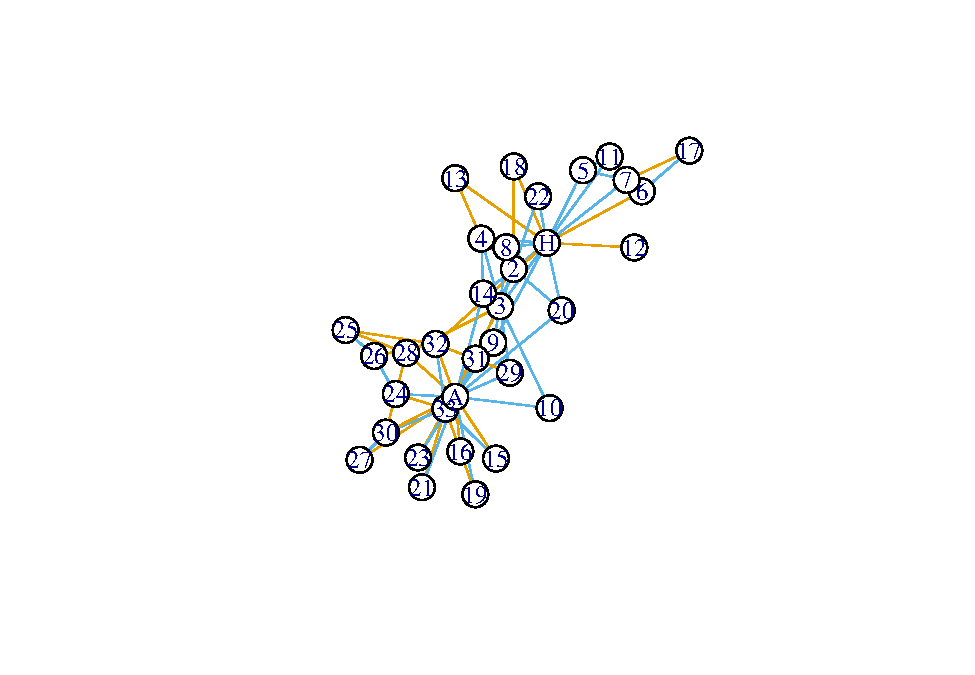
\includegraphics{bookdown-demo_files/figure-latex/unnamed-chunk-184-1.pdf}

\begin{Shaded}
\begin{Highlighting}[]
\FunctionTok{plot}\NormalTok{(karate, }\AttributeTok{vertex.color =} \StringTok{\textquotesingle{}white\textquotesingle{}}\NormalTok{, }\AttributeTok{edge.color =} \FunctionTok{c}\NormalTok{(}\StringTok{\textquotesingle{}red\textquotesingle{}}\NormalTok{, }\StringTok{\textquotesingle{}blue\textquotesingle{}}\NormalTok{)[}\FunctionTok{factor}\NormalTok{(}\FunctionTok{E}\NormalTok{(karate)}\SpecialCharTok{$}\NormalTok{edge\_type)]) }\CommentTok{\# specifying your own colors }
\end{Highlighting}
\end{Shaded}

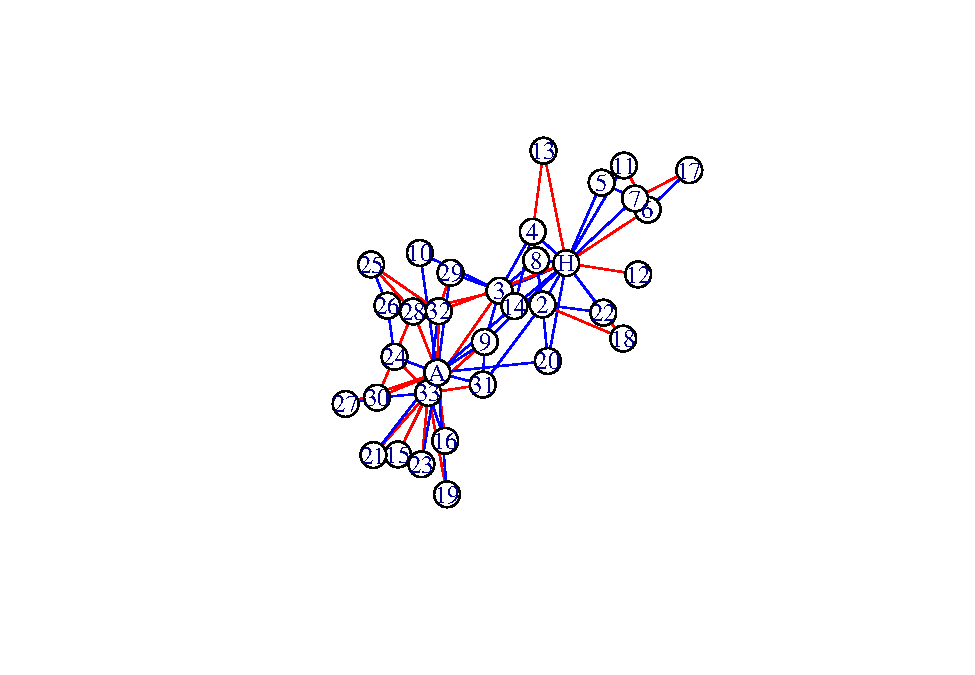
\includegraphics{bookdown-demo_files/figure-latex/unnamed-chunk-184-2.pdf}

\begin{Shaded}
\begin{Highlighting}[]
\FunctionTok{factor}\NormalTok{(}\FunctionTok{E}\NormalTok{(karate)}\SpecialCharTok{$}\NormalTok{edge\_type) }\SpecialCharTok{|\textgreater{}} \FunctionTok{levels}\NormalTok{() }\CommentTok{\# this tells you the ordering of the levels so you can tell that red = different and blue = same }
\end{Highlighting}
\end{Shaded}

\begin{verbatim}
## [1] "different" "same"
\end{verbatim}

\subsection{Edge thickness based on their continuous attributes}\label{edge-thickness-based-on-their-continuous-attributes}

\begin{Shaded}
\begin{Highlighting}[]
\FunctionTok{plot}\NormalTok{(karate, }\AttributeTok{vertex.color =} \StringTok{\textquotesingle{}white\textquotesingle{}}\NormalTok{, }\AttributeTok{edge.width =} \FunctionTok{E}\NormalTok{(karate)}\SpecialCharTok{$}\NormalTok{weight)}
\end{Highlighting}
\end{Shaded}

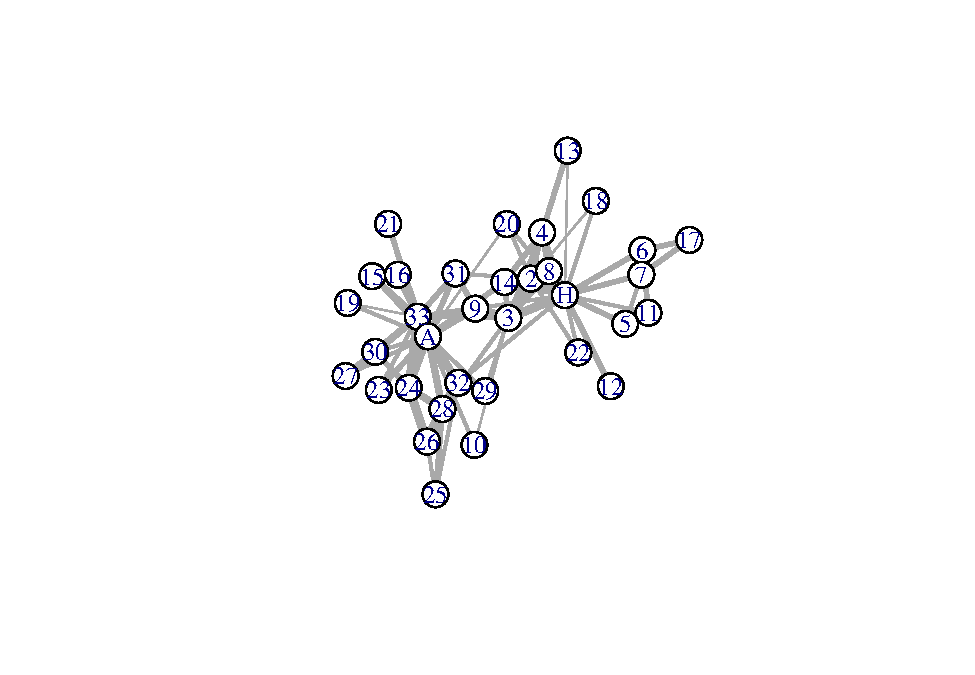
\includegraphics{bookdown-demo_files/figure-latex/unnamed-chunk-185-1.pdf}

\subsection{Arrows for directed edges}\label{arrows-for-directed-edges}

\begin{Shaded}
\begin{Highlighting}[]
\FunctionTok{plot}\NormalTok{(}\FunctionTok{as.directed}\NormalTok{(karate, }\AttributeTok{mode =} \StringTok{\textquotesingle{}random\textquotesingle{}}\NormalTok{), }\AttributeTok{vertex.color =} \StringTok{\textquotesingle{}white\textquotesingle{}}\NormalTok{, }\AttributeTok{edge.arrow.width =} \FloatTok{0.5}\NormalTok{, }\AttributeTok{edge.arrow.size =} \FloatTok{0.5}\NormalTok{)}
\end{Highlighting}
\end{Shaded}

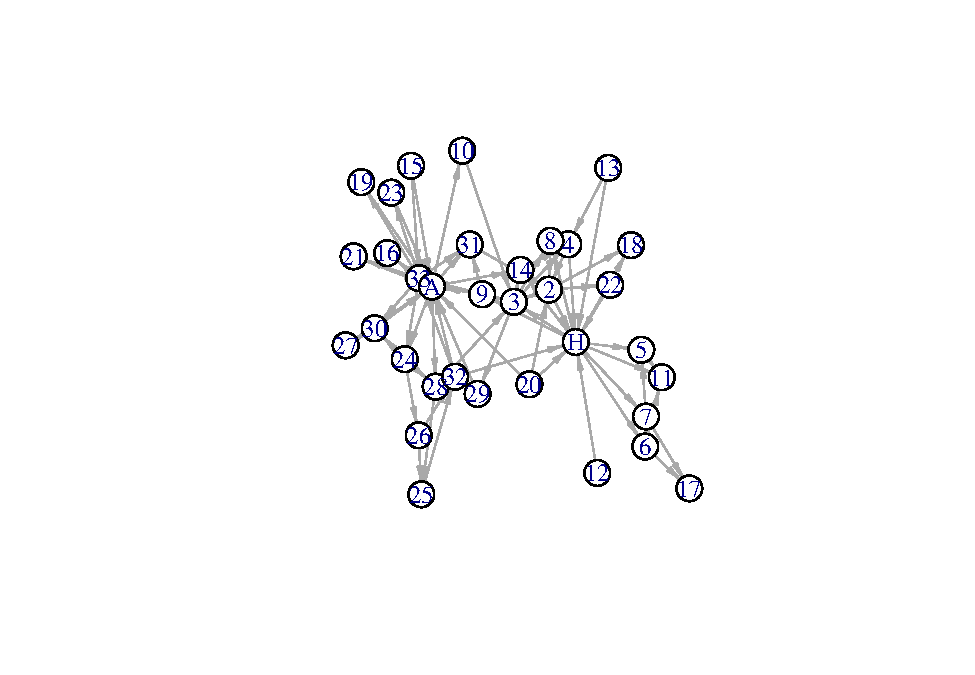
\includegraphics{bookdown-demo_files/figure-latex/unnamed-chunk-186-1.pdf}

\section{Other}\label{other}

\subsection{Graph layouts}\label{graph-layouts}

It is good practice to set a seed before executing the graph layout functions, so that you are able to ``save'' the output and replicate it in the future. Notice that the layout function takes the network as its argument and outputs a 2 column matrix which is the x- and y-coordinates for each of the nodes in the network (explore the \texttt{my\_layout1} R object). Then you can insert that as the input to the layout parameter when you want to plot the network.

\begin{Shaded}
\begin{Highlighting}[]
\DocumentationTok{\#\# saving a fixed layout for future use }
\FunctionTok{set.seed}\NormalTok{(}\DecValTok{1}\NormalTok{)}
\NormalTok{my\_layout1 }\OtherTok{\textless{}{-}} \FunctionTok{layout\_in\_circle}\NormalTok{(karate)}

\FunctionTok{set.seed}\NormalTok{(}\DecValTok{2}\NormalTok{)}
\NormalTok{my\_layout2 }\OtherTok{\textless{}{-}} \FunctionTok{layout\_with\_dh}\NormalTok{(karate)}

\FunctionTok{plot}\NormalTok{(karate, }\AttributeTok{layout =}\NormalTok{ my\_layout1)}
\end{Highlighting}
\end{Shaded}

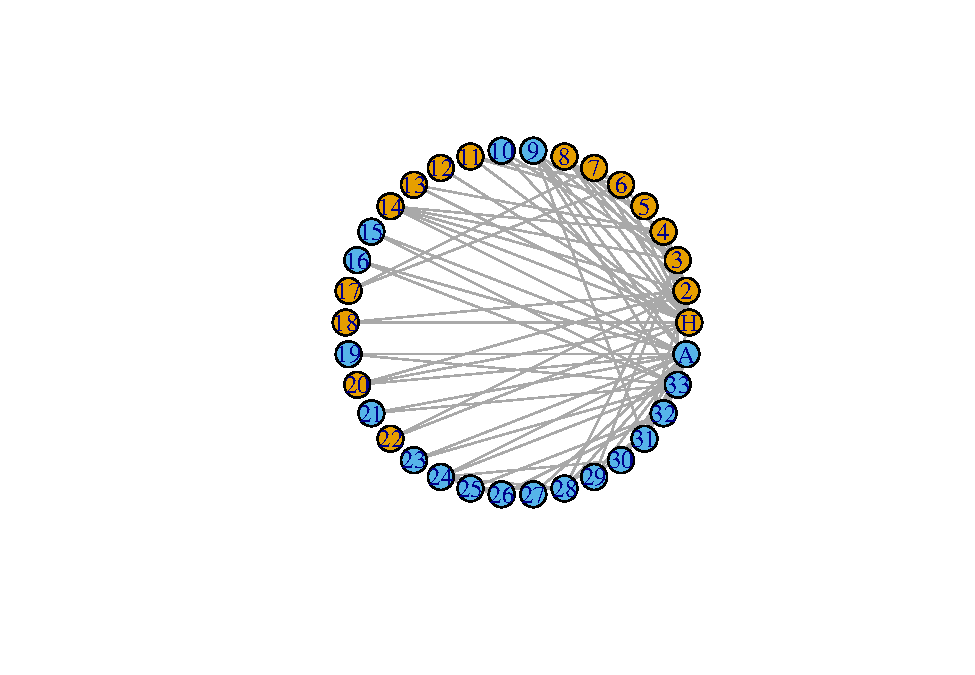
\includegraphics{bookdown-demo_files/figure-latex/unnamed-chunk-187-1.pdf}

\begin{Shaded}
\begin{Highlighting}[]
\FunctionTok{plot}\NormalTok{(karate, }\AttributeTok{layout =}\NormalTok{ my\_layout2)}
\end{Highlighting}
\end{Shaded}

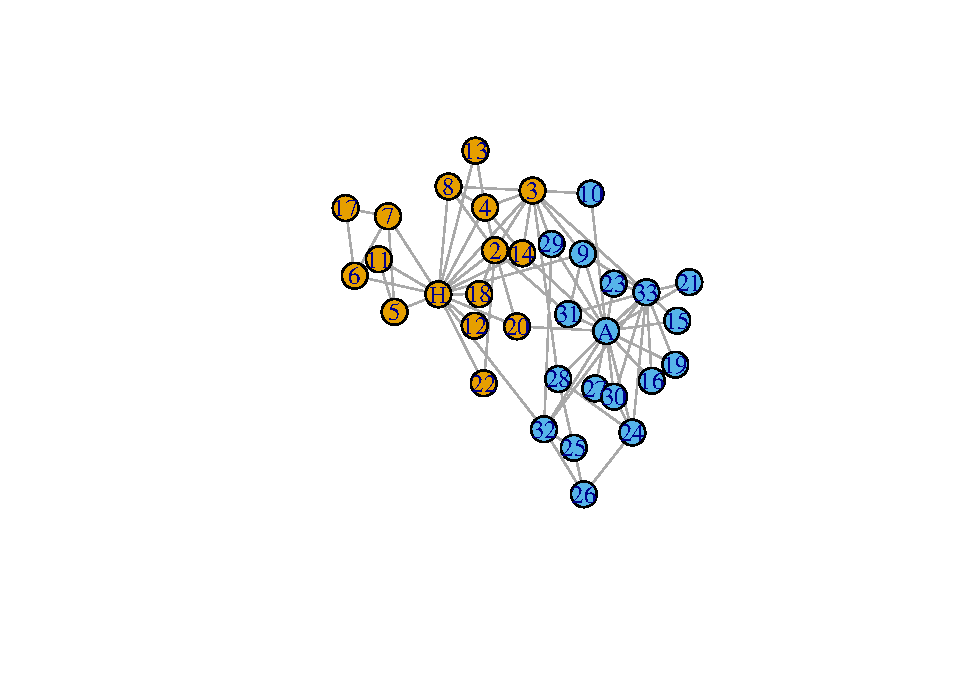
\includegraphics{bookdown-demo_files/figure-latex/unnamed-chunk-187-2.pdf}

See \url{https://kateto.net/network-visualization} (Section 4.2 Network layouts) to learn more about the different plotting formats available in \texttt{igraph}.

\subsection{Plot title}\label{plot-title}

\begin{Shaded}
\begin{Highlighting}[]
\DocumentationTok{\#\# add a plot title {-}{-}{-}{-}}
\FunctionTok{plot}\NormalTok{(karate, }\AttributeTok{vertex.color =} \FunctionTok{V}\NormalTok{(karate)}\SpecialCharTok{$}\NormalTok{community, }\AttributeTok{main =} \StringTok{\textquotesingle{}Communities in the karate network\textquotesingle{}}\NormalTok{)}
\end{Highlighting}
\end{Shaded}

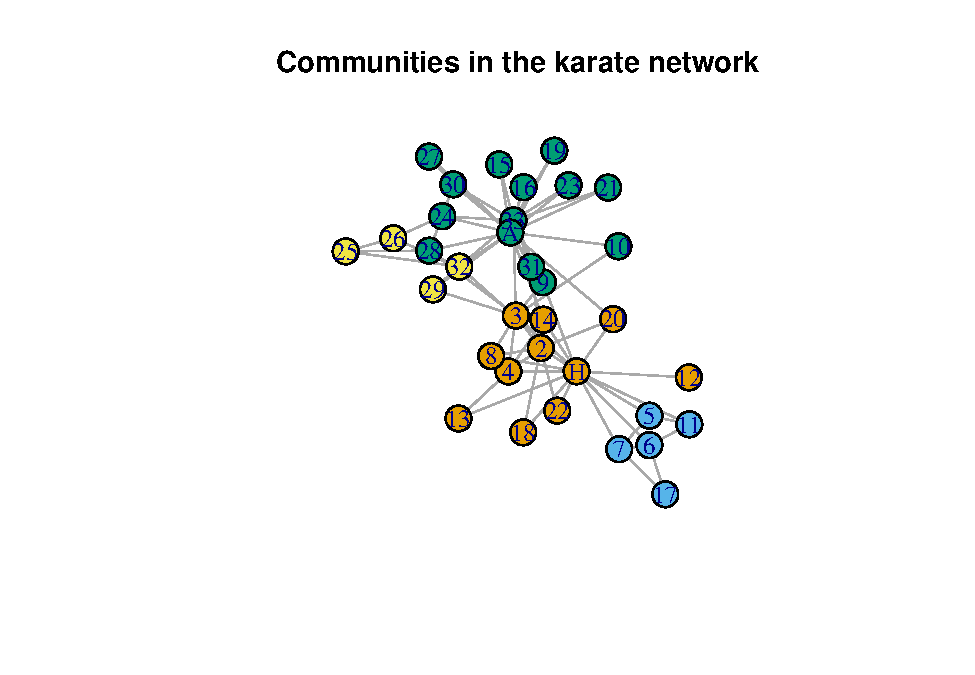
\includegraphics{bookdown-demo_files/figure-latex/unnamed-chunk-188-1.pdf}

\subsection{Add a subtitle}\label{add-a-subtitle}

\begin{Shaded}
\begin{Highlighting}[]
\DocumentationTok{\#\# add a subtitle {-}{-}{-}{-}}
\FunctionTok{plot}\NormalTok{(karate, }\AttributeTok{vertex.color =} \FunctionTok{V}\NormalTok{(karate)}\SpecialCharTok{$}\NormalTok{community, }\AttributeTok{main =} \StringTok{\textquotesingle{}Communities in the karate network\textquotesingle{}}\NormalTok{,}
     \AttributeTok{sub =} \StringTok{\textquotesingle{}The Louvain community detection method was used.\textquotesingle{}}\NormalTok{)}
\end{Highlighting}
\end{Shaded}

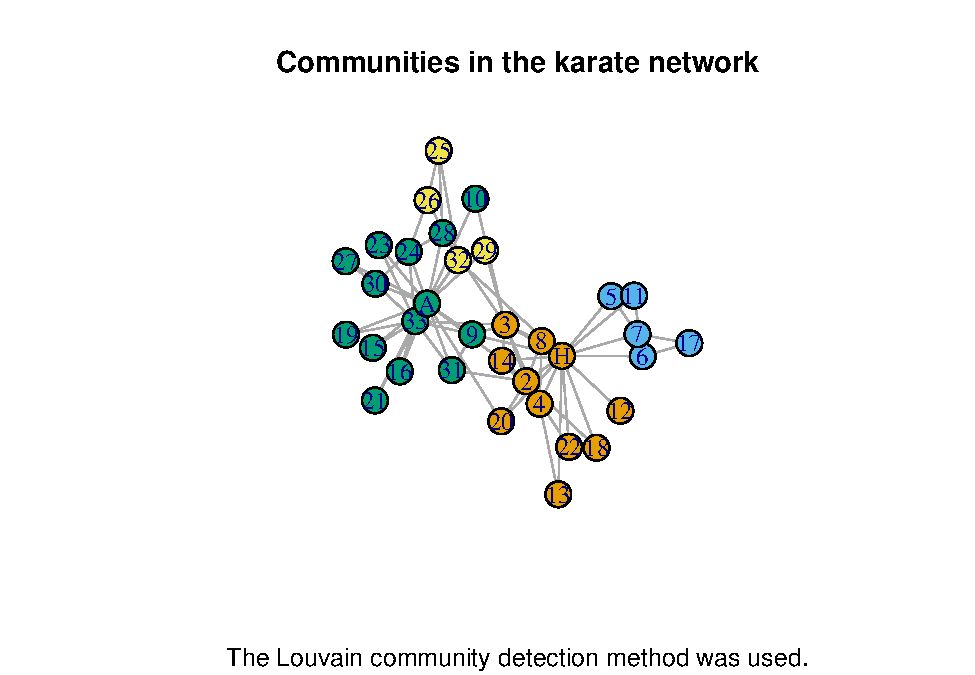
\includegraphics{bookdown-demo_files/figure-latex/unnamed-chunk-189-1.pdf}

\subsection{Multiple plots}\label{multiple-plots}

\begin{Shaded}
\begin{Highlighting}[]
\DocumentationTok{\#\# multiple plots {-}{-}{-}{-}}

\FunctionTok{par}\NormalTok{(}\AttributeTok{mar=}\FunctionTok{c}\NormalTok{(}\DecValTok{0}\NormalTok{,}\DecValTok{0}\NormalTok{,}\DecValTok{0}\NormalTok{,}\DecValTok{0}\NormalTok{)}\SpecialCharTok{+}\DecValTok{1}\NormalTok{, }\AttributeTok{mfrow =} \FunctionTok{c}\NormalTok{(}\DecValTok{1}\NormalTok{,}\DecValTok{2}\NormalTok{)) }\CommentTok{\# adjust margins, 1 row, 2 columns  }

\FunctionTok{plot}\NormalTok{(karate, }\AttributeTok{layout =}\NormalTok{ my\_layout1, }\AttributeTok{main =} \StringTok{\textquotesingle{}layout 1\textquotesingle{}}\NormalTok{)}
\FunctionTok{plot}\NormalTok{(karate, }\AttributeTok{layout =}\NormalTok{ my\_layout2, }\AttributeTok{main =} \StringTok{\textquotesingle{}layout 2\textquotesingle{}}\NormalTok{)}
\end{Highlighting}
\end{Shaded}

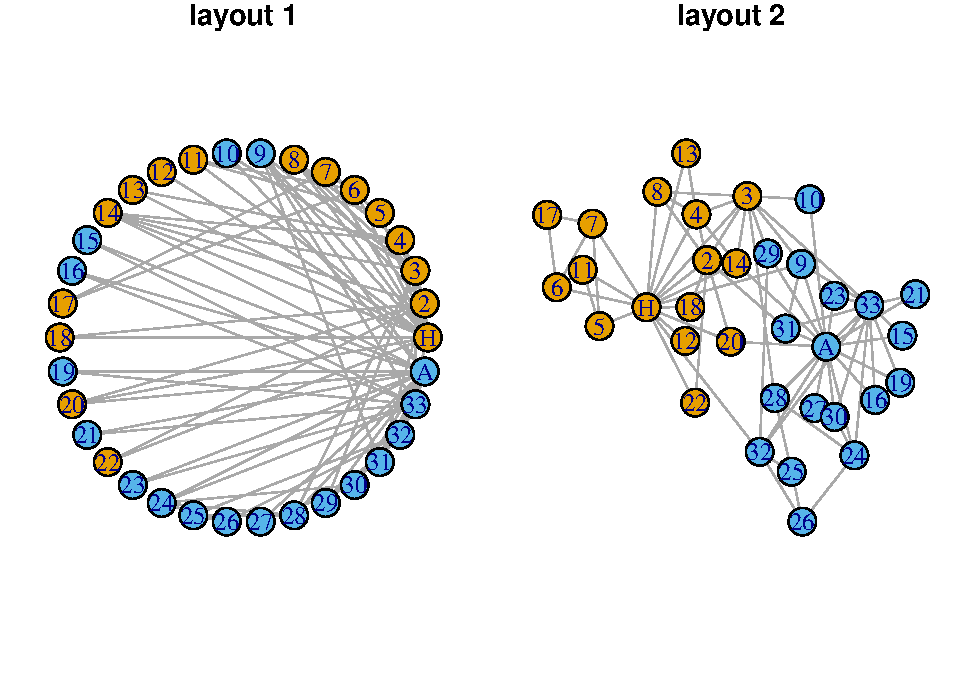
\includegraphics{bookdown-demo_files/figure-latex/unnamed-chunk-190-1.pdf}

\subsection{Useful links}\label{useful-links}

Introduction to network visualization in R: \url{https://kateto.net/network-visualization}

Colors in R: \url{https://r-charts.com/colors/}

\chapter{Chapter 15: Network visualization with other packages}\label{ch15}

Under construction.

Planned topics:
- gephi
- networkD3
- threejs
- visNetwork

\chapter{Chapter 16: Analyzing degree distributions}\label{ch16}

Early work in the era of modern network science has revealed that the degree distributions of real-world networks followed a power-law (Barabasi \& Albert, 2002). This was an important discovery because the fact that a power law could characterize the distribution of node degrees across a wide, diverse range of networks suggested that a common mechanism or organizing principle could be responsible for such a pattern. This led Barabasi and colleagues to propose a prominent model of network growth, known as \emph{preferential attachment}, that provided a possible mechanism for the emergence of a power law degree distributions in networks.

However, we need to first understand two concepts before proceeding: \emph{degree distribution} and \emph{power law}.

\emph{Degree distribution} refers to the probability distribution of node degrees in a given network. For instance, what proportion of nodes in the network have a degree of \(x\), where \(x\) represents various degree values in the network?

\emph{Power law} is a class of long-tailed distributions where the relationship between two variables is best characterized by an exponent (power relation). If a degree distribution follows a power law, the relation between the probability distribution of node degrees and the value of the degree itself is characterized by an exponential function, as follows:

\(p(x) = Cx^{-\alpha}\)

Where \(p(x)\) is the probability of \(x\) occurring in the dataset, \(C\) = a constant, \(\alpha\) = exponent or power of the relationship between \(x\) and \(p(x)\). The exponent is negative because it is a negative relationship: As \(x\) (node degree) increases, the probability (of it occurring) decreases. This mathematical relationship captures the idea that hubs (nodes with extremely high degree) are more uncommon in the network than nodes with lower degree.

In this Chapter, we will work through an example of how to analyze the distribution of a variable, and to statistically assess if its distribution is indeed similar to a power law distribution. The example is drawn from the tutorials provided by the creator of the \texttt{poweRlaw} R package, see the vignettes on \url{https://cran.r-project.org/web/packages/poweRlaw/index.html} for a more detailed walk through.

\section{Set up}\label{set-up-4}

First, let's make sure to download and then load the \texttt{poweRLaw} R package into our workspace.

\begin{Shaded}
\begin{Highlighting}[]
\CommentTok{\# install.packages(\textquotesingle{}poweRlaw\textquotesingle{})}

\FunctionTok{library}\NormalTok{(}\StringTok{\textquotesingle{}poweRlaw\textquotesingle{}}\NormalTok{)}
\end{Highlighting}
\end{Shaded}

For this example, we will use the Moby Dick data set provided in the \texttt{poweRlaw} package. The \texttt{moby} R object is a vector of numbers, which each number corresponds to the raw frequency count of words found in the novel Moby Dick. The vector is also organized from the most frequently occurring word, to the least frequently occurring word. Notice that the identity of the words was not provided in the vector, but usually function words are the most frequently words in language corpora (e.g., the, of, to, etc.). Finally, although the example is on word frequencies, the same procedure can be applied to any quantity, e.g.~node degrees in the network.

\begin{Shaded}
\begin{Highlighting}[]
\FunctionTok{data}\NormalTok{(}\StringTok{"moby"}\NormalTok{, }\AttributeTok{package =} \StringTok{"poweRlaw"}\NormalTok{)}

\FunctionTok{head}\NormalTok{(moby)}
\end{Highlighting}
\end{Shaded}

\begin{verbatim}
## [1] 14086  6414  6260  4573  4484  4040
\end{verbatim}

\begin{Shaded}
\begin{Highlighting}[]
\FunctionTok{tail}\NormalTok{(moby)}
\end{Highlighting}
\end{Shaded}

\begin{verbatim}
## [1] 1 1 1 1 1 1
\end{verbatim}

\section{Fitting the power law distribution}\label{fitting-the-power-law-distribution}

Then, we run the following code to fit the data to a power law distribution and infer two key parameters, alpha and \(x_{min}\).

\begin{Shaded}
\begin{Highlighting}[]
\CommentTok{\# assign a power law distribution "object" to the data }
\NormalTok{m\_pl }\OtherTok{=}\NormalTok{ displ}\SpecialCharTok{$}\FunctionTok{new}\NormalTok{(moby) }

\CommentTok{\# infer parameters (alpha, minimum cut off)}
\NormalTok{est }\OtherTok{=} \FunctionTok{estimate\_xmin}\NormalTok{(m\_pl) }
\NormalTok{est}
\end{Highlighting}
\end{Shaded}

\begin{verbatim}
## $gof
## [1] 0.008252634
## 
## $xmin
## [1] 7
## 
## $pars
## [1] 1.952728
## 
## $ntail
## [1] 2958
## 
## $distance
## [1] "ks"
## 
## attr(,"class")
## [1] "estimate_xmin"
\end{verbatim}

\begin{Shaded}
\begin{Highlighting}[]
\CommentTok{\# update the power law object with parameters }
\NormalTok{m\_pl}\SpecialCharTok{$}\FunctionTok{setXmin}\NormalTok{(est) }
\NormalTok{m\_pl}
\end{Highlighting}
\end{Shaded}

\begin{verbatim}
## Reference class object of class "displ" 
## Field "xmin": 
## [1] 7
## Field "pars": 
## [1] 1.952728
## Field "no_pars": 
## [1] 1
\end{verbatim}

The output looks a bit crazy! Let's try to unpack it. The first output \texttt{est} contains the results of fitting the power law distribution to the word frequency data. \texttt{\$gof} tells us the goodness of fit statistic as estimated from using the Kolmogorov-Smirnov test to measure the distance between the actual distribution and the fitted power law distribution. \texttt{\$pars} is the alpha exponent of the power law distribution. \texttt{\$xmin} tells us the cut off point at which the power law up to. You can think of this as the part of the distribution where there is a lot of jitter and noise (common in real world data) and the power law is not fitted to the data where \(x\) is less than that cut off. In the last part of the code, we plug these estimated values back into the power law object; this is to enable us to conduct statistical testing later on.

\section{Visualization}\label{visualization}

We can also visualize the fitted power law distribution (in red; notice how the line does not continue beyond \(x_{min}\) \textless{} 7), plotted on log-log scale. The (negative) slope of the best-fit line corresponds to the alpha (exponent) parameter.

\begin{Shaded}
\begin{Highlighting}[]
\CommentTok{\# visualization }
\FunctionTok{plot}\NormalTok{(m\_pl)}
\FunctionTok{lines}\NormalTok{(m\_pl, }\AttributeTok{col =} \StringTok{\textquotesingle{}red\textquotesingle{}}\NormalTok{) }
\end{Highlighting}
\end{Shaded}

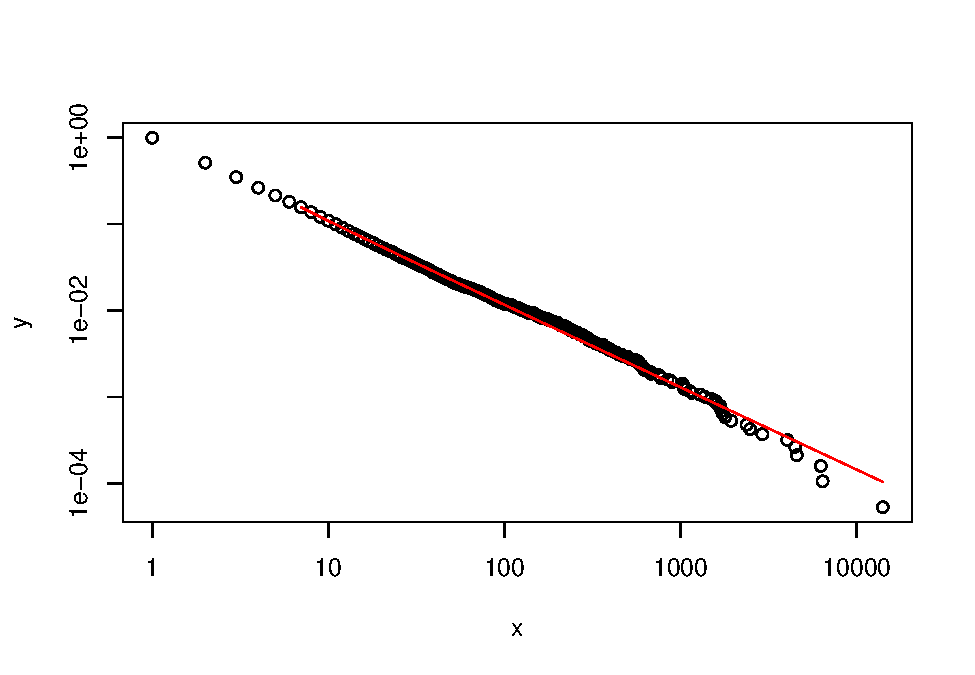
\includegraphics{bookdown-demo_files/figure-latex/unnamed-chunk-194-1.pdf}

\section{Statistical testing of distribution fit}\label{statistical-testing-of-distribution-fit}

\subsection{Method 1: Bootstrapping the data}\label{method-1-bootstrapping-the-data}

Because it is possible to fit a power-law distribution to any data set, Clauset et al.~strongly recommend that we test whether the observed data set actually follows a power-law. The method used below follows Clauset et al.'s suggestion to test the null hypothesis (that the data came from a power law distribution) using a goodness-of-fit test with a bootstrapping procedure. The basic concept is to perform a hypothesis test by generating multiple data sets (with the previously estimated parameters \(x_{min}\) and alpha) and then ``re-inferring'' the model parameters. The original model parameter is then compared to the simulated set of parameters. If the p-value is greater than .05, we cannot reject the null hypothesis that the data could be generated from a power law distribution with similar parameters. If the p-value is less than .05, we reject the null hypothesis, and conclude that the data is not convincingly fit by a power law.

\begin{Shaded}
\begin{Highlighting}[]
\CommentTok{\# parameter uncertainty and statistical testing }

\DocumentationTok{\#\# 1000 bootstraps using four cores}
\NormalTok{bs\_p }\OtherTok{=} \FunctionTok{bootstrap\_p}\NormalTok{(m\_pl, }\AttributeTok{no\_of\_sims =} \DecValTok{1000}\NormalTok{, }\AttributeTok{threads =} \DecValTok{4}\NormalTok{, }\AttributeTok{seed =} \DecValTok{1}\NormalTok{) }\CommentTok{\# can be slow}
\end{Highlighting}
\end{Shaded}

\begin{verbatim}
## Expected total run time for 1000 sims, using 4 threads is 217 seconds.
\end{verbatim}

\begin{Shaded}
\begin{Highlighting}[]
\NormalTok{bs\_p}\SpecialCharTok{$}\NormalTok{bootstraps }\SpecialCharTok{|\textgreater{}} \FunctionTok{head}\NormalTok{()}
\end{Highlighting}
\end{Shaded}

\begin{verbatim}
##           gof xmin     pars ntail
## 1 0.009839299    6 1.917765  3515
## 2 0.007466091   10 1.969352  2095
## 3 0.009205848    9 1.943017  2290
## 4 0.013751881    7 1.942744  2989
## 5 0.004895829    6 1.956929  3469
## 6 0.008659503    7 1.952541  2943
\end{verbatim}

\begin{Shaded}
\begin{Highlighting}[]
\FunctionTok{mean}\NormalTok{(bs\_p}\SpecialCharTok{$}\NormalTok{bootstraps[, }\DecValTok{2}\NormalTok{]) }\CommentTok{\# M of xmin}
\end{Highlighting}
\end{Shaded}

\begin{verbatim}
## [1] 7.668
\end{verbatim}

\begin{Shaded}
\begin{Highlighting}[]
\FunctionTok{mean}\NormalTok{(bs\_p}\SpecialCharTok{$}\NormalTok{bootstraps[, }\DecValTok{3}\NormalTok{]) }\CommentTok{\# M of pars (alpha)}
\end{Highlighting}
\end{Shaded}

\begin{verbatim}
## [1] 1.950474
\end{verbatim}

\begin{Shaded}
\begin{Highlighting}[]
\FunctionTok{sd}\NormalTok{(bs\_p}\SpecialCharTok{$}\NormalTok{bootstraps[, }\DecValTok{2}\NormalTok{]) }\CommentTok{\# SD of xmin}
\end{Highlighting}
\end{Shaded}

\begin{verbatim}
## [1] 3.341398
\end{verbatim}

\begin{Shaded}
\begin{Highlighting}[]
\FunctionTok{sd}\NormalTok{(bs\_p}\SpecialCharTok{$}\NormalTok{bootstraps[, }\DecValTok{3}\NormalTok{]) }\CommentTok{\# SD of pars (alpha)}
\end{Highlighting}
\end{Shaded}

\begin{verbatim}
## [1] 0.02341784
\end{verbatim}

\begin{Shaded}
\begin{Highlighting}[]
\FunctionTok{hist}\NormalTok{(bs\_p}\SpecialCharTok{$}\NormalTok{bootstraps[, }\DecValTok{2}\NormalTok{])}
\end{Highlighting}
\end{Shaded}

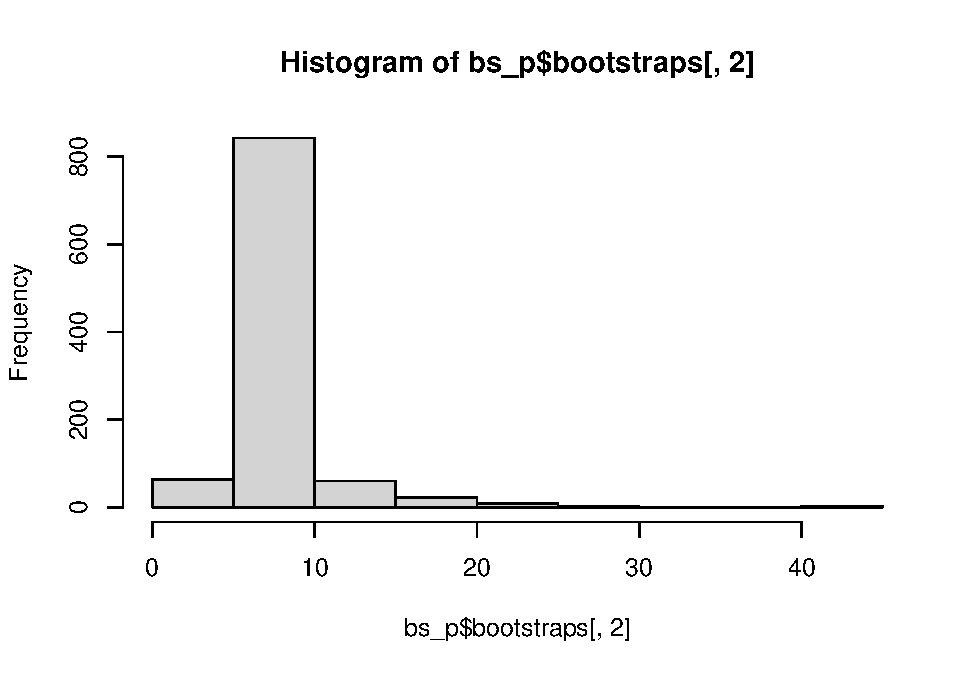
\includegraphics{bookdown-demo_files/figure-latex/unnamed-chunk-195-1.pdf}

\begin{Shaded}
\begin{Highlighting}[]
\FunctionTok{hist}\NormalTok{(bs\_p}\SpecialCharTok{$}\NormalTok{bootstraps[, }\DecValTok{3}\NormalTok{])}
\end{Highlighting}
\end{Shaded}

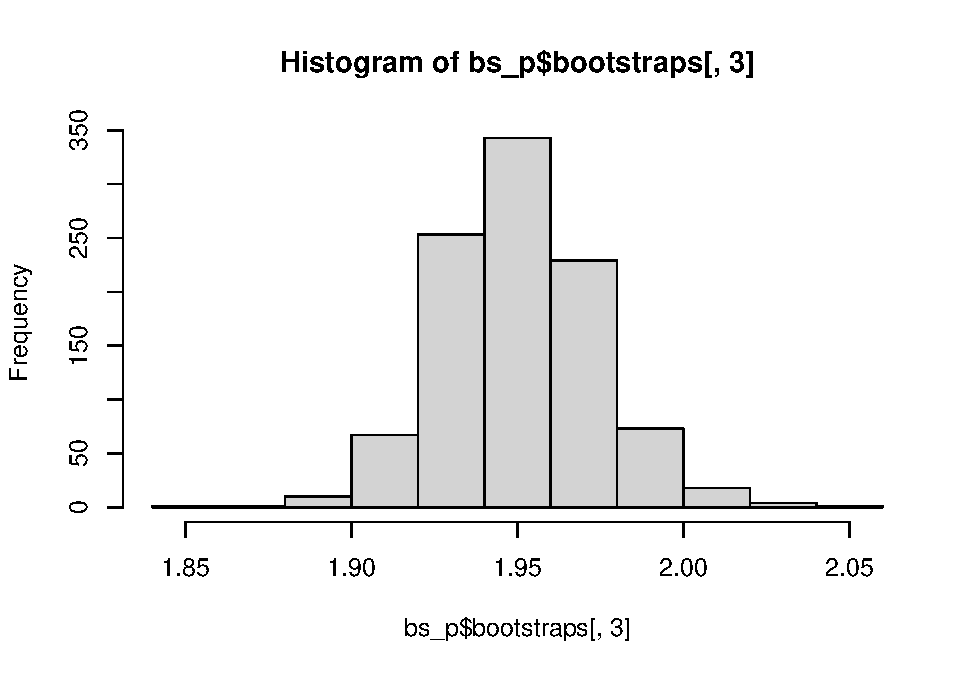
\includegraphics{bookdown-demo_files/figure-latex/unnamed-chunk-195-2.pdf}

\begin{Shaded}
\begin{Highlighting}[]
\CommentTok{\# p{-}value }
\NormalTok{bs\_p}\SpecialCharTok{$}\NormalTok{p }\CommentTok{\# null hypothesis: distribution came from a power law distribution, since p \textgreater{} 0.05, cannot reject the null  }
\end{Highlighting}
\end{Shaded}

\begin{verbatim}
## [1] 0.694
\end{verbatim}

\subsection{Method 2: Comparing alternative distributions}\label{method-2-comparing-alternative-distributions}

An alternative method is to fit other long-tailed distributions to the data, and then compare these distributions directly using a likelihood ratio test. The code below shows you how to compare the power law distribution to the log-normal distribution (although other long-tailed distributions can also be tested). Basically, there is a similar process of fitting the data to the new distribution and updating the parameters. Then the \texttt{compare\_distributions} function is used to provide a likelihood ratio test comparing the two distributions. Since the test was not statistically significant, both distributions are equally far from the true distribution and hence it is not possible to determine which is the best fitting model.

\begin{Shaded}
\begin{Highlighting}[]
\CommentTok{\# make a log{-}normal object for moby }
\CommentTok{\# fix the xmin parameter to be the same as m\_pl }
\NormalTok{m\_ln }\OtherTok{\textless{}{-}}\NormalTok{ dislnorm}\SpecialCharTok{$}\FunctionTok{new}\NormalTok{(moby)}
\NormalTok{m\_ln}\SpecialCharTok{$}\FunctionTok{setXmin}\NormalTok{(}\DecValTok{7}\NormalTok{)}

\CommentTok{\# estimate the parameters for log normal distribution }
\NormalTok{est }\OtherTok{\textless{}{-}} \FunctionTok{estimate\_pars}\NormalTok{(m\_ln)}

\CommentTok{\# update the parameters into the object }
\NormalTok{m\_ln}\SpecialCharTok{$}\FunctionTok{setPars}\NormalTok{(est)}

\CommentTok{\# use Vuong\textquotesingle{}s test to compare PL vs LN distributions }
\NormalTok{comp }\OtherTok{\textless{}{-}} \FunctionTok{compare\_distributions}\NormalTok{(m\_pl, m\_ln)}

\NormalTok{comp}\SpecialCharTok{$}\NormalTok{p\_two\_sided}
\end{Highlighting}
\end{Shaded}

\begin{verbatim}
## [1] 0.6773366
\end{verbatim}

\section{Exercise}\label{exercise-9}

Analyze the degree distribution of the following network:

\begin{Shaded}
\begin{Highlighting}[]
\FunctionTok{library}\NormalTok{(igraphdata)}

\FunctionTok{data}\NormalTok{(}\StringTok{\textquotesingle{}UKfaculty\textquotesingle{}}\NormalTok{)}
\end{Highlighting}
\end{Shaded}

To get a vector of ``degree counts'' (c.f., word frequencies in Moby Dick), use the following code and see if this degree distribution follows a power law distribution using the bootstrapping approach.

\begin{Shaded}
\begin{Highlighting}[]
\NormalTok{degree\_frequencies }\OtherTok{\textless{}{-}} \FunctionTok{table}\NormalTok{(}\FunctionTok{degree}\NormalTok{(UKfaculty, }\AttributeTok{mode =} \StringTok{\textquotesingle{}all\textquotesingle{}}\NormalTok{))}
\end{Highlighting}
\end{Shaded}

\section{References}\label{references-3}

For an example of how this approach has been used to explore the degree distributions of networks, see:

Siew, C. S. Q., \& Vitevitch, M. S. (2020). Investigating the Influence of Inverse Preferential Attachment on Network Development. \emph{Entropy, 22}(9), Article 9. \url{https://doi.org/10.3390/e22091029}

Clauset, A., Shalizi, C. R., \& Newman, M. E. (2009). Power-law distributions in empirical data. \emph{SIAM Review, 51}(4), 661--703.

Gillespie, C. S. (2015). PoweRlaw: Analysis of heavy tailed distributions. R Package Version 0.30. 0, URL \url{Http://CRAN}. R-Project. Org/Package= poweRlaw.

  \bibliography{book.bib,packages.bib}

\end{document}
